%%%%%%%%%%%%%%%%%%%%%%%%%%%%%%%%%%%%%%%%%%
% Mathematics Final Year Research Projects
% LaTeX Template
% Version 1.0 (31/01/24)
%
% This template has been adapted from: https://www.overleaf.com/latex/templates/imperial-college-report-template/wncnzptkhnbc
% Students should feel free to adapt this template to their needs.
%%%%%%%%%%%%%%%%%%%%%%%%%%%%%%%%%%%%%%%%%%
%----------------------------------------------------------------------------------------
% PACKAGES AND OTHER DOCUMENT CONFIGURATIONS
%----------------------------------------------------------------------------------------

% IMPORTANT NOTE: This version of the document is NOT the one I'm submitting. This is a significantly longer version that contains several important details that can later be added to the blueprint. The text here, particularly in Chapter 4, is meant to mimic the arguments that we have and will formalise.

\documentclass[a4paper,11pt, twoside]{report}
\usepackage[T1]{fontenc}
\usepackage[utf8]{inputenc}

%% Language and font encodings
\usepackage[english]{babel}
\usepackage[utf8]{inputenc}
\usepackage[T1]{fontenc}

%% Imperial Recommended Packages
\usepackage{afterpage}

% Lean colour configurations
\usepackage{color}
\definecolor{keywordcolor}{rgb}{0.7, 0.1, 0.1}   % red
\definecolor{tacticcolor}{rgb}{0.0, 0.1, 0.6}    % blue
\definecolor{commentcolor}{rgb}{0.4, 0.4, 0.4}   % grey
\definecolor{symbolcolor}{rgb}{0.0, 0.1, 0.6}    % blue
\definecolor{sortcolor}{rgb}{0.1, 0.5, 0.1}      % green
\definecolor{attributecolor}{rgb}{0.7, 0.1, 0.1} % red
\definecolor{backcolour}{rgb}{0.95,0.95,0.92}

% Listings (for displaying code):
\usepackage{listings}
\def\lstlanguagefiles{TeX_Setup/lstlean.tex}
\lstset{
    % frame = single, 
    % framexleftmargin=15pt,
    language = lean,
    numbers = left,
    backgroundcolor=\color{backcolour}
}

% ----------- Algorithm2e setup
\usepackage[ruled,vlined]{algorithm2e}
\makeatletter
\renewcommand{\SetKwInOut}[2]{%
  \sbox\algocf@inoutbox{\KwSty{#2}\algocf@typo:}%
  \expandafter\ifx\csname InOutSizeDefined\endcsname\relax% if first time used
    \newcommand\InOutSizeDefined{}\setlength{\inoutsize}{\wd\algocf@inoutbox}%
    \sbox\algocf@inoutbox{\parbox[t]{\inoutsize}{\KwSty{#2}\algocf@typo:\hfill}~}\setlength{\inoutindent}{\wd\algocf@inoutbox}%
  \else% else keep the larger dimension
    \ifdim\wd\algocf@inoutbox>\inoutsize%
    \setlength{\inoutsize}{\wd\algocf@inoutbox}%
    \sbox\algocf@inoutbox{\parbox[t]{\inoutsize}{\KwSty{#2}\algocf@typo:\hfill}~}\setlength{\inoutindent}{\wd\algocf@inoutbox}%
    \fi%
  \fi% the dimension of the box is now defined.
  \algocf@newcommand{#1}[1]{%
    \ifthenelse{\boolean{algocf@inoutnumbered}}{\relax}{\everypar={\relax}}%
%     {\let\\\algocf@newinout\hangindent=\wd\algocf@inoutbox\hangafter=1\parbox[t]{\inoutsize}{\KwSty{#2}\algocf@typo\hfill:}~##1\par}%
    {\let\\\algocf@newinout\hangindent=\inoutindent\hangafter=1\parbox[t]{\inoutsize}{\KwSty{#2}\algocf@typo:\hfill}~##1\par}%
    \algocf@linesnumbered% reset the numbering of the lines
  }}%
\makeatother
% --------- end algorithm2e setup

\usepackage{bm}
\usepackage[normalem]{ulem}

\usepackage[colorinlistoftodos]{todonotes}

% I have all of their other recommended packages somewhere on here.

\usepackage[most]{tcolorbox}
\usepackage{authblk}  % Lets you add an \affil{} to your title, stating your affiliation {eg. Sigma Mathematics Society}
\usepackage{ragged2e}
\usepackage{csquotes}
\usepackage{pdfpages}



\usepackage{xfrac}
\usepackage{cancel}

\usepackage[inline]{enumitem}

%\usepackage{tgpagella}

\usepackage{blindtext}
\usepackage{lipsum}
\usepackage{verbatim}
\usepackage{hyperref}
\hypersetup{
    citebordercolor = 1 1 1,
    linkbordercolor = 1 1 1,
    filebordercolor = 1 1 1,
    menubordercolor = 1 1 1,
    urlbordercolor = 1 1 1,
    colorlinks  =   true,
    linkcolor   =   blue,
    citecolor   =   magenta,
    urlcolor    =   blue
}

% This project uses natbib instead. See end of format file.
% \usepackage{biblatex} % Modify citation format using [style=yourstyle] parameter--eg \usepackage[style=mla-new]{biblatex}
% \bibliography{TeX_Setup/References.bib}
% \addbibresource{TeX_Setup/References.bib}

\usepackage{cancel}
\usepackage{amssymb}
\usepackage{amsmath}
% \usepackage{amsthm}  % In `environments.tex`
%\usepackage{MnSymbol}
\usepackage{mathrsfs}
\usepackage{mathtools}
% \usepackage{mathabx}
\usepackage{mathdots}
\usepackage{yhmath}

\usepackage{array}
\usepackage{booktabs}
\usepackage{longtable}

\usepackage{graphicx}
\newcommand\sbullet[1][.5]{\mathbin{\vcenter{\hbox{\scalebox{#1}{$\bullet$}}}}}  % Bullet of customisable size
\usepackage{wrapfig}
% Imperial-recommended `caption` setup
\usepackage{caption}
\captionsetup[figure]{labelfont={bf}, name={Figure}, justification=centering}
\captionsetup[table]{labelfont={bf}, name={Table}}
\usepackage{subcaption}
\usepackage{tikz}
\usepackage{float}

% Tikz
\usepackage{tikz-cd}
\usepackage{tikz-3dplot}
\usetikzlibrary{positioning}
\usetikzlibrary{cd}
\usetikzlibrary{shapes.geometric}
\usepackage{pgfplots}
\usepackage{mathrsfs}
\usetikzlibrary{arrows}
\usepackage{qtree}

%% Sets page size and margins
\usepackage[a4paper,top=1in,bottom=1in,left=1in,right=1in,marginparwidth=1.75cm]{geometry}

% Font

% \usepackage{sansmathfonts}
% % \usepackage{mathrsfs}
% \usepackage[T1]{fontenc}
% \renewcommand*\familydefault{\sfdefault}

\renewcommand*{\rmdefault}{bch}
\renewcommand*{\ttdefault}{lmtt}

% Structure and Numbering

\usepackage{fancyhdr}
\usepackage{lastpage}

\pagestyle{fancy}
\fancyhf{}

\rhead{{Page \thepage}}%\hspace{1pt} of \pageref{LastPage}}}
\lhead{\textit\slshape\nouppercase{\leftmark}}

\numberwithin{equation}{section}

% Lists

\setlist[description]{font=\normalfont}
\setlist[enumerate]{before=\normalfont}

% Spacing and indentation

% Not sure if 1.5-spacing is permitted. I'll leave it commented out for now.
% \usepackage{setspace}
% \renewcommand{\baselinestretch}{1.5}

\usepackage[skip=11pt, indent=0pt]{parskip}
% Here's what Imperial's recommended setup is:
% \setlength{\parskip}{0.5em}
% \usepackage{indentfirst}  % Uncomment if using above

\allowdisplaybreaks  % Allows align environments to continue for several pages

% Colours

\usepackage{xcolor}
\definecolor{darkblue}{rgb}{0.0, 0.0, 0.55}
\definecolor{pink}{rgb}{0.858, 0.188, 0.478}
\definecolor{brown}{rgb}{0.8, 0.4, 0.0}

% Bibliography
\usepackage[numbers, comma, square, sort&compress]{natbib}
\bibliographystyle{References/abbrvunsrtnat.bst}
% \bibliographystyle{unsrtnat}

\usepackage{amsthm}
% Gives theorem and definition names the same font style as the words "theorem"/"definition": see https://tex.stackexchange.com/questions/43966/how-to-make-the-optional-title-of-a-theorem-bold-with-amsthm
\makeatletter
\def\th@plain{%
  \thm@notefont{}% same as heading font
  \itshape % body font
}
\def\th@definition{%
  \thm@notefont{}% same as heading font
  \normalfont % body font
}
\makeatother

\usepackage{cleveref}

\newtheorem*{theorem*}{Theorem}
\newtheorem{theorem}{Theorem}[section]
\newtheorem{corollary}[theorem]{Corollary}%[theorem]
\newtheorem{lemma}[theorem]{Lemma}
\newtheorem{claim}[theorem]{Claim}
\newtheorem{conjecture}[theorem]{Conjecture}
% \newtheorem{algorithm}[theorem]{Algorithm}  % Defined in algorithm2e
\newtheorem{proposition}[theorem]{Proposition}

\newtheorem{problem}[theorem]{Problem}
\newenvironment{boxproblem}{
    \begin{tcolorbox}[colback=yellow!15!white,colframe=orange, breakable, enhanced]\begin{problem}
}{
    \end{problem}\end{tcolorbox}
}

\newenvironment{boxtheorem}{
    \begin{tcolorbox}[colback=yellow!15!white,colframe=orange, breakable, enhanced]\begin{theorem}
}{
    \end{theorem}\end{tcolorbox}
}
\newenvironment{boxproposition}{
    \begin{tcolorbox}[colback=yellow!15!white,colframe=orange, breakable, enhanced]\begin{proposition}
}{
    \end{proposition}\end{tcolorbox}
}
\newenvironment{boxlemma}{
    \begin{tcolorbox}[colback=yellow!15!white,colframe=orange, breakable, enhanced]\begin{lemma}
}{
    \end{lemma}\end{tcolorbox}
}
\newenvironment{boxcorollary}{
    \begin{tcolorbox}[colback=yellow!15!white,colframe=orange, breakable, enhanced]\begin{corollary}
}{
    \end{corollary}\end{tcolorbox}
}
\newenvironment{boxconjecture}{
    \begin{tcolorbox}[colback=yellow!15!white,colframe=orange, breakable, enhanced]\begin{conjecture}
}{
    \end{conjecture}\end{tcolorbox}
}


\theoremstyle{remark}
\newtheorem*{remark}{Remark}
\newtheorem*{solution}{Solution}

\theoremstyle{definition}
\newtheorem{definition}[theorem]{Definition}
\newenvironment{boxdefinition}{
    \begin{tcolorbox}[colback=cyan!10!white,colframe=cyan!70!black, breakable, enhanced]\begin{definition}
}{
    \end{definition}\end{tcolorbox}
}
\newtheorem*{convention}{Convention}
\newenvironment{boxconvention}{
    \begin{tcolorbox}[colback=magenta!3!white,colframe=magenta!70!black, breakable, enhanced]\begin{convention}
}{
    \end{convention}\end{tcolorbox}
}
\newtheorem*{notation}{Notation}
\newenvironment{boxnotation}{
    \begin{tcolorbox}[colback=magenta!3!white,colframe=magenta!70!black, breakable, enhanced]\begin{notation}
}{
    \end{notation}\end{tcolorbox}
}
\newtheorem{example}[theorem]{Example}
\newenvironment{boxexample}{
    \begin{tcolorbox}[colframe=green!30!black, breakable, enhanced, breakable, enhanced]\begin{example}
}{
    \end{example}\end{tcolorbox}
}
\newtheorem{nexample}[theorem]{Non-Example}
\newenvironment{boxnexample}{
    \begin{tcolorbox}[colframe=red!50!black, breakable, enhanced]\begin{nexample}
}{
    \end{nexample}\end{tcolorbox}
}
\newtheorem{cexample}[theorem]{Counterexample}
\newenvironment{boxcexample}{
    \begin{tcolorbox}[colframe=red!50!black, breakable, enhanced]\begin{cexample}
}{
    \end{cexample}\end{tcolorbox}
}

% \def\SMALLCOLWIDTH{1.5cm}
\newcolumntype{C}[1]{>{\centering\let\newline\\\arraybackslash\hspace{0pt}}m{#1}}

% Centering captions
% \renewcommand{\caption}[1]{\caption{\centering #1}}

%%%%%%%%%%%%%%%%%%%%%%%%%%%%%%%%%%%%%%%%%%%%%%%%%%%%%%%%%%%%%%%%%%%%%%%%%%%%%%%%%%%%%%%%%%%%%%%%%%%%%%%%%%%%
% CUSTOM COMMANDS
%%%%%%%%%%%%%%%%%%%%%%%%%%%%%%%%%%%%%%%%%%%%%%%%%%%%%%%%%%%%%%%%%%%%%%%%%%%%%%%%%%%%%%%%%%%%%%%%%%%%%%%%%%%%

% Custom colours

\definecolor{darkgreen}{rgb}{0.1, 0.4, 0.3}      % green

% `sorry`

\newcommand{\sorry}{\textcolor{red}{\texttt{sorry}}}
% \newcommand{\sorry}{\lstinline{sorry}}

% TIKZ:

\newcommand{\drawplane}{  % For use with TikZ
    \draw[step=0.5cm,gray,very thin] (-2.5,-2.5) grid (2.5,2.5);
    \draw[thick,->] (-2.5,0) -- (2.5,0); % node[anchor=west] {$x$};
    \draw[thick,->] (0,-2.5) -- (0,2.5); % node[anchor=south] {$y$};
    % \node[black, anchor=north east] at (0, 0) {$0$};
}
\newcommand{\latticecircle}[2]{
    \draw[fill=yellow, opacity=0.5] (#1, #2) circle (0.5);
    \node at (#1, #2) {\color{gray}{$\bullet$}};
}
\newcommand{\latticecirclegrey}[2]{
    \draw[fill=gray, opacity=0.75] (#1, #2) circle (0.5);
    \node at (#1, #2) {\color{black}{$\bullet$}};
}
\newcommand{\latticecirclebrown}[2]{
    \draw[fill=brown, opacity=0.75] (#1, #2) circle (0.5);
    \node at (#1, #2) {\color{black}{$\bullet$}};
}
\usetikzlibrary{decorations.markings}
\tikzset{->-/.style={decoration={
      markings,
      mark=at position #1 with {\arrow{>}}},postaction={decorate}
}}

\newenvironment{cd}{
    \begin{equation} \begin{tikzcd}
}{
    \end{tikzcd} \end{equation}
}
\newenvironment{cd*}{
    \begin{equation*} \begin{tikzcd}
}{
    \end{tikzcd} \end{equation*}
}

\newcommand{\drawsquare}[1]{
    \draw[thick, blue]
    (-{#1},-{#1}) node [anchor=north east] {C} --
    (-{#1}, {#1}) node[anchor=south east] {B} --
    ({#1}, {#1}) node[anchor=south west] {A} --
    ({#1}, -{#1}) node [anchor=north west] {D} -- cycle;
}

\newcommand{\labelledpoint}[5]{ % Takes x coord, y coord, label x-position relative to point, label y-position relative to point, label text as arguments
    \node [label={[shift={(#3,#4)}]#5}] at (#1, #2) {$\bullet$};
}

% DELIMITERS:

\newcommand{\parenth}[1]{\left( #1 \right)}
\newcommand{\brac}[1]{\left[ #1 \right]}
\newcommand{\set}[1]{\left\{ #1 \right\}}
\newcommand{\setst}[2]{\set{#1 \; \middle\vert \; #2}}
\newcommand{\abs}[1]{\left\lvert #1 \right\rvert}
\newcommand{\norm}[1]{\left\lVert #1 \right\rVert}
\newcommand{\floor}[1]{\left\lfloor #1 \right\rfloor}
\newcommand{\ceil}[1]{\left\lceil #1 \right\rceil}
\newcommand{\cycl}[1]{\left\langle #1 \right\rangle}
\newcommand{\grpres}[2]{\cycl{#1 \; \middle| \; #2}}  % \grpres{gens}{rels}

% FUNCTIONS:

\newcommand{\fx}{f\!\parenth{x}}
\newcommand{\fof}[1]{f\!\parenth{#1}}

\newcommand{\px}{p\!\parenth{x}}
\newcommand{\pof}[1]{p\!\parenth{#1}}
\newcommand{\pofbig}[1]{p\Big(#1\Big)}
\newcommand{\gx}{g\!\parenth{x}}
\newcommand{\gof}[1]{g\!\parenth{#1}}
\newcommand{\hx}{h\!\parenth{x}}
\newcommand{\hof}[1]{h\!\parenth{#1}}
\newcommand{\Tv}{T\!\parenth{v}}
\newcommand{\Tof}[1]{T\!\parenth{#1}}
\newcommand{\Tbar}{\overline{T}}
\newcommand{\Tbarof}[1]{\Tbar\!\parenth{#1}}
\newcommand{\Tbarv}{\Tbarof{v}}
\newcommand{\Sof}[1]{S\!\parenth{#1}}

\newcommand{\psin}[1]{\sin\!{\parenth{#1}}}
\newcommand{\pcos}[1]{\cos\!{\parenth{#1}}}
\newcommand{\ptan}[1]{\tan\!{\parenth{#1}}}
\newcommand{\sinsq}[1]{\sin^2\!\parenth{#1}}
\newcommand{\cossq}[1]{\cos^2\!\parenth{#1}}
\newcommand{\tansq}[1]{\tan^2\!\parenth{#1}}
\newcommand{\parcsin}[1]{\arcsin\!{\parenth{#1}}}
\newcommand{\parccos}[1]{\arccos\!{\parenth{#1}}}
\newcommand{\parctan}[1]{\arctan\!{\parenth{#1}}}

\newcommand{\logbase}[2]{\log_{#1}\!\parenth{#2}}
\newcommand{\nthroot}[2]{\sqrt[\leftroot{-3}\uproot{3} #1]{#2}}
\newcommand{\cbrt}[1]{\nthroot{3}{#1}}

\newcommand{\pgcd}[2]{\gcd\!\parenth{{#1},{#2}}}
\newcommand{\plcm}[2]{\operatorname{lcm}\!\parenth{{#1},{#2}}}
\newcommand{\pgcds}[1]{\gcd\!\parenth{#1}}
\newcommand{\plcms}[1]{\operatorname{lcm}\!\parenth{#1}}

\newcommand{\varphiof}[1]{\varphi\!\parenth{#1}}
\newcommand{\phiof}[1]{\phi\!\parenth{#1}}
\newcommand{\xiof}[1]{\xi\!\parenth{#1}}
\newcommand{\rhoof}[1]{\rho\!\parenth{#1}}
\newcommand{\pexp}[1]{\exp\!\parenth{#1}}

\newcommand{\inj}{\hookrightarrow}
\newcommand{\surj}{\twoheadrightarrow}

\DeclareMathOperator*{\argmin}{\arg\!\min}
\DeclareMathOperator*{\argmax}{\arg\!\max}

\newcommand{\of}[1]{\!\parenth{#1}}

% CALCULUS:

\newcommand{\dx}{\operatorname{d}\!x}
\newcommand{\dy}{\operatorname{d}\!y}
\newcommand{\diff}[1]{\operatorname{d}\!{#1}}
\newcommand{\dydx}{\frac{\dy}{\dx}}

% LINEAR ALGEBRA:

\newcommand{\mat}[3]{\operatorname{M}_{{#1} \times {#2}}\!\parenth{{#3}}}
\newcommand{\matsq}[2]{\operatorname{M}_{{#1} \times {#1}}\!\parenth{\mathbb{#2}}}
\newcommand{\MnR}{\operatorname{M}_{n}\!\parenth{\real}}
\newcommand{\MnC}{\operatorname{M}_{n}\!\parenth{\C}}
\newcommand{\Mn}[2]{\operatorname{M}_{#1}\!\parenth{#2}}
\newcommand{\GL}[1]{\operatorname{GL}\!\parenth{#1}}
\newcommand{\SL}[1]{\operatorname{SL}\!\parenth{#1}}
\newcommand{\PGL}[1]{\operatorname{PGL}\!\parenth{#1}}
\newcommand{\PSL}[1]{\operatorname{PSL}\!\parenth{#1}}

\newcommand{\Span}[1]{\operatorname{Span}\!\parenth{#1}}

\newcommand{\pdim}[1]{\dim\!\parenth{#1}}

\newcommand{\RSp}[1]{\operatorname{RSp}\!\parenth{#1}}
\newcommand{\CSp}[1]{\operatorname{CSp}\!\parenth{#1}}
\newcommand{\rank}[1]{\operatorname{rank}\!\parenth{#1}}
\newcommand{\pim}[1]{\operatorname{im}\!\parenth{#1}}
\newcommand{\pker}[1]{\operatorname{ker}\!\parenth{#1}}
\newcommand{\pdet}[1]{\det\!\parenth{#1}}

\newcommand{\cA}[1]{c_A \! \parenth{#1}}
\newcommand{\cB}[1]{c_B \! \parenth{#1}}
\newcommand{\mA}[1]{m_A \! \parenth{#1}}
\newcommand{\mB}[1]{m_B \! \parenth{#1}}
\newcommand{\cAx}{\cA{x}}
\newcommand{\cBx}{\cB{x}}
\newcommand{\mAx}{\mA{x}}
\newcommand{\mBx}{\mB{x}}
\newcommand{\cof}[2]{c_{#1}\!\parenth{#2}}
\newcommand{\mof}[2]{m_{#1}\!\parenth{#2}}

\newcommand{\Cof}[1]{C\!\parenth{#1}}
\newcommand{\+}{\oplus}
\newcommand{\pdeg}[1]{\deg\!\parenth{#1}}

\newcommand{\RCF}[1]{\operatorname{RCF}\!\parenth{#1}}
\newcommand{\JCF}[1]{\operatorname{JCF}\!\parenth{#1}}

\newcommand{\Jsub}[2]{J_{#1}\!\parenth{#2}}

\newcommand{\Aof}[1]{A\!\parenth{#1}}

\newcommand{\Tsub}[2]{T_{#1}\!\parenth{#2}}

\newcommand{\Tr}[1]{\operatorname{Tr}\!\parenth{#1}}

\newcommand{\diag}[1]{\operatorname{diag}\!\parenth{#1}}

% Measure Theory

\newcommand{\muof}[1]{\mu\!\parenth{#1}}
\newcommand{\muA}{\muof{A}}
\newcommand{\muB}{\muof{B}}
\newcommand{\mutof}[1]{\Tilde{\mu}\!\parenth{#1}}
\newcommand{\mustof}[1]{\mu^*\!\parenth{#1}}
\newcommand{\calF}{\mathcal{F}}
\newcommand{\calA}{\mathcal{A}}
\newcommand{\calB}{\mathcal{B}}
\newcommand{\calC}{\mathcal{C}}
\newcommand{\sigmaof}[1]{\sigma\!\parenth{#1}}
\newcommand{\psiof}[1]{\psi\!\parenth{#1}}

% Intervals

\newcommand{\Ioc}[1]{\left(#1\right]}
\newcommand{\Ico}[1]{\left[#1\right)}

% GROUPS/ALGEBRA IN GENERAL:

\newcommand{\inv}{^{-1}}
\newcommand{\Sym}[1]{\operatorname{Sym}\!\parenth{#1}}
\newcommand{\ord}[1]{\operatorname{ord}\!\parenth{#1}}
\newcommand{\supp}[1]{\operatorname{supp}\!\parenth{#1}}
\newcommand{\sgn}[1]{\operatorname{sgn}\!\parenth{#1}}
\newcommand{\tcyc}[2]{\begin{pmatrix} #1 & #2 \end{pmatrix}}

\newcommand{\nsg}{\trianglelefteq}

\newcommand{\Rmul}{R^{\times}}
\newcommand{\kmul}{k^{\times}}
\newcommand{\kX}{k\!\brac{X}}
\newcommand{\RX}{R\!\brac{X}}

\newcommand{\quotient}[2]{
    \left.\raisebox{.2em}{${#1}$} \middle/ \raisebox{-.2em}{${#2}$} \right.
}
\newcommand{\Zmod}[1]{\quotient{\Z}{{#1}\Z}}

\newcommand{\Vof}[1]{V\!\parenth{#1}}

\newcommand{\Frac}[1]{\operatorname{Frac}\!\parenth{#1}}

\newcommand{\Spec}[1]{\operatorname{Spec}\!\parenth{#1}}

\newcommand{\id}{\operatorname{id}}

\newcommand{\pchar}[1]{\operatorname{char}\!\parenth{#1}}

\newcommand{\Hom}{\operatorname{Hom}}

\newcommand{\Zof}[1]{\operatorname{Z}\!\parenth{#1}}

\newcommand{\Aut}[1]{\operatorname{Aut}\!\parenth{#1}}

% NUMBER SETS:

\newcommand{\real}{\mathbb{R}}
\newcommand{\rational}{\mathbb{Q}}
\newcommand{\naturalnum}{\mathbb{N}}
\newcommand{\integers}{\mathbb{Z}}
\newcommand{\complex}{\mathbb{C}}

\newcommand{\Field}{\mathbb{F}}
\newcommand{\Q}{\mathbb{Q}}
\newcommand{\R}{\real}
\newcommand{\N}{\naturalnum}
\newcommand{\Z}{\integers}
\newcommand{\C}{\complex}
\newcommand{\B}{\mathcal{B}}
\newcommand{\I}{\mathcal{I}}
\newcommand{\J}{\mathcal{J}}

\newcommand{\psup}[1]{\sup\!\parenth{#1}}
\newcommand{\pinf}[1]{\inf\!\parenth{#1}}

% LOGIC:

\newcommand{\ergo}{\therefore}
\newcommand{\bcos}{\because}
\newcommand{\st}{\text{ s.t. }}


% -------------------- SPECIFIC TO PROJECT -------------------- %

% TERMINOLOGY

\newcommand{\CELP}{Cohn-Elkies Linear Programming Bound}
\newcommand{\CEC}{Cohn-Elkies Conditions}
\newcommand{\JCT}{Jordan Curve Theorem}
\newcommand{\CGT}{Cauchy-Goursat Theorem}

% NOTATION

\newcommand{\Pa}{\mathcal{P}}
\newcommand{\Vol}{\operatorname{Vol}}
\newcommand{\Volof}[1]{\Vol\!\parenth{#1}}
\newcommand{\Sch}{\mathcal{S}}
\renewcommand{\hat}{\widehat}
\renewcommand{\tilde}{\widetilde}
\newcommand{\F}{\mathcal{F}}
\newcommand{\periodic}{\operatorname{periodic}}

\newcommand{\Halfplane}{\mathbb{H}} % Using Lean notation for the upper-half plane instead of Viazovska's

\newcommand{\BigO}[1]{\operatorname{O}\of{#1}}

\newcommand{\fm}{f \mid}
\newcommand{\fmof}[3]{\parenth{\fm_{#1} {#2}}\of{#3}}

% COMPLEX ANALYSIS

\renewcommand{\Re}{\operatorname{Re}}
\renewcommand{\Im}{\operatorname{Im}}

\newcommand{\rad}{_{\operatorname{rad}}}

% LEAN

\newcommand{\mathlib}{\texttt{mathlib}}


% %% Useful packages
% \usepackage{afterpage}
% \usepackage{amsmath}
% \usepackage{amsthm}
% \usepackage{amssymb}
% \usepackage{csquotes}
% \usepackage{enumitem}
% \usepackage{graphicx}
% \usepackage{lipsum}
% \usepackage{booktabs}

% % Listings (for displaying code):
% \usepackage{listings}
% \lstset{
%     frame = single, 
%     framexleftmargin=15pt
% }

% % Center figure captions:
% \usepackage{caption}
% \captionsetup[figure]{labelfont={bf},name={Figure},labelsep=quad}
% \captionsetup[table]{labelfont={bf},name={Table},labelsep=quad}


% % ----------- Algorithm2e setup
% \usepackage[ruled,vlined]{algorithm2e}
% \makeatletter
% \renewcommand{\SetKwInOut}[2]{%
%   \sbox\algocf@inoutbox{\KwSty{#2}\algocf@typo:}%
%   \expandafter\ifx\csname InOutSizeDefined\endcsname\relax% if first time used
%     \newcommand\InOutSizeDefined{}\setlength{\inoutsize}{\wd\algocf@inoutbox}%
%     \sbox\algocf@inoutbox{\parbox[t]{\inoutsize}{\KwSty{#2}\algocf@typo:\hfill}~}\setlength{\inoutindent}{\wd\algocf@inoutbox}%
%   \else% else keep the larger dimension
%     \ifdim\wd\algocf@inoutbox>\inoutsize%
%     \setlength{\inoutsize}{\wd\algocf@inoutbox}%
%     \sbox\algocf@inoutbox{\parbox[t]{\inoutsize}{\KwSty{#2}\algocf@typo:\hfill}~}\setlength{\inoutindent}{\wd\algocf@inoutbox}%
%     \fi%
%   \fi% the dimension of the box is now defined.
%   \algocf@newcommand{#1}[1]{%
%     \ifthenelse{\boolean{algocf@inoutnumbered}}{\relax}{\everypar={\relax}}%
% %     {\let\\\algocf@newinout\hangindent=\wd\algocf@inoutbox\hangafter=1\parbox[t]{\inoutsize}{\KwSty{#2}\algocf@typo\hfill:}~##1\par}%
%     {\let\\\algocf@newinout\hangindent=\inoutindent\hangafter=1\parbox[t]{\inoutsize}{\KwSty{#2}\algocf@typo:\hfill}~##1\par}%
%     \algocf@linesnumbered% reset the numbering of the lines
%   }}%
% \makeatother
% % --------- end algorithm2e setup

% % \bm allows typing bold math:
% \usepackage{bm}
% \usepackage[normalem]{ulem}

% \usepackage[colorinlistoftodos]{todonotes}
% \usepackage[colorlinks=true, allcolors=blue]{hyperref}

% \renewcommand*{\rmdefault}{bch}
% \renewcommand*{\ttdefault}{lmtt}
% \newcommand{\citationneeded}{\textcolor{red}{[citation-needed]}}

% % Add bigger skip between paragraphs, makes reading easier:
% \setlength{\parskip}{0.5em}

% % Bibliography
% \usepackage[numbers, comma, square, sort&compress]{natbib}
% \bibliographystyle{References/abbrvunsrtnat.bst}

%----------------------------------------------------------------------------------------
% END OF DOCUMENT CONFIGURATION
%----------------------------------------------------------------------------------------

%----------------------------------------------------------------------------------------
% IMPORTANT INFORMATION TO MODIFY FOR THE TITLE PAGE
%----------------------------------------------------------------------------------------
\newcommand{\reporttitle}{Viazovska's Magic Function in Dimension 8: \\ An Attempt at Formalisation} % Title of your research project
\newcommand{\reportauthor}{Sidharth Hariharan} % First Name and Last Name
\newcommand{\supervisor}{Bhavik Mehta} % First Name and Last Name of your supervisor(s)
\newcommand{\degreetype}{MSci in Mathematics} % MSci in Mathematics, BSc in Mathematics, BSc in Mathematics with Statistics, ...
%----------------------------------------------------------------------------------------

%----------------------------------------------------------------------------------------
% To compile this file, use the following sequence: 
%	latex main.tex
%	bibtex main.tex
%	latex main.tex
%	latex main.tex
%----------------------------------------------------------------------------------------

%----------------------------------------------------------------------------------------
% START OF DOCUMENT
%----------------------------------------------------------------------------------------
\begin{document}

% Title page
\begin{titlepage}

\newcommand{\HRule}{\rule{\linewidth}{0.5mm}} % Defines a new command for the horizontal lines, change thickness here

%----------------------------------------------------------------------------------------
%	LOGO SECTION
%----------------------------------------------------------------------------------------


\includegraphics[width=8cm]{Title/logo.png}\\[1cm] % Include a department/university logo - this will require the graphicx package
 
%----------------------------------------------------------------------------------------

\center % Center everything on the page

%----------------------------------------------------------------------------------------
%	HEADING SECTIONS
%----------------------------------------------------------------------------------------

% For M3R or M4R reports, comment out as appropriate
\textsc{\LARGE Imperial College London}\\[0.5cm] % Name of your university/college
\textsc{\Large Department of Mathematics}\\[1.5cm] % Name of your department
\textsc{\Large MSci Research Project}\\[0.5cm] % Name of your programme
%\textsc{\LARGE BSc Research Project}\\[1.5cm] 

%----------------------------------------------------------------------------------------
%	TITLE SECTION
%----------------------------------------------------------------------------------------
\makeatletter
\HRule \\[0.6cm]
{ \huge \bfseries \reporttitle}\\[0.6cm] % Title of your document
\HRule \\[1.5cm]
 
%----------------------------------------------------------------------------------------
%	AUTHOR SECTION
%----------------------------------------------------------------------------------------

\begin{minipage}{0.4\textwidth}
\begin{flushleft} \large
\emph{Author:}\\
\reportauthor % Your name
\end{flushleft}
\end{minipage}
~
\begin{minipage}{0.4\textwidth}
\begin{flushright} \large
\emph{Supervisor(s):} \\
\supervisor % Supervisor's name
\end{flushright}
\end{minipage}\\[2cm]
\makeatother

%----------------------------------------------------------------------------------------
%	FOOTER & DATE SECTION
%----------------------------------------------------------------------------------------
\vfill % Fill the rest of the page with whitespace
Submitted in partial fulfillment of the requirements for the \degreetype~at Imperial College London\\[0.5cm]

\makeatletter
{\large \today}\\[2cm] % Date, change the \today to a set date if you want to be precise
\makeatother

\end{titlepage}

% Abstract
\thispagestyle{empty}
\begin{abstract}
    Hi
\end{abstract}
 
% % Acknowledgements
% \clearpage
% \thispagestyle{empty}
\section*{Acknowledgments}

\textit{I would like to dedicate this project to my two beloved Thathas, both of whom attained Moksha during my time at Imperial. While I knew your beginnings were humble, I wish I had realised, when you were still in this world, just how much you did so that your children could have better opportunities than you. As have they, I shall ever strive to pay it forward, and completing this degree is the first step towards doing that. Not a day goes by when I do not miss you, and I will forever be grateful for all you have given me. Om Shanti.}

To my supervisor, Bhavik, I am beyond grateful for your guidance and support throughout this project. I would never have thought a chance encounter in Lausanne would lead to a working relationship that would so significantly impact my professional outlook. You have given me new standards to aspire to early on in my career, with your sharpness of mind and vastness of knowledge. Beyond a supervisor, you have been an incredible mentor and gave me great advice when I was applying to PhD positions. From the bottom of my heart, thank you.

I would further like to express my thanks to Kevin Buzzard for having not only introduced me to Lean but for never having stopped encouraging me since I attended my first Xena Project session in October 2021. I am especially grateful to you for having simultaneously hyped me up for this very high-profile project and fended off the FRO's requests to take the project public before the M4R deadline.

I would be remiss without thanking the great Maryna Viazovska herself, for whose work I have developed the profoundest appreciation over the course of this project. Even beyond that, your incredible warmth and approachability demonstrate that the greatest mathematicians are also great human beings. It has been my life's greatest honour to work with you.

I am grateful to the entire Lean community, particularly those based in London, and within that subset, those who attend Xena. I would particularly like to express my thanks to Heather Macbeth for her riveting metaprogramming sessions, one of which led to \lstinline|norm_numI|, and Edison Xie, for conversations, company, Lean brainstorming, and the occasional Michelin-star dinner.

Amma, Appa, I do not even know where I would begin. From listening to me ramble about abstract nonsense to sharing in all my joys and sadnesses, you are more than just the pillars of my world: you are my world. All I do, all I am, all I will be are because you made me so. I was blessed to be born to you.

Finally, I wish to thank everyone from my Wilkinson and maths family who has made Imperial feel like home. To my very first maths friends, Dev and Jaimin, thank you for the laughs, the vibes, and above all, for the solidarity. Without the two of you, Tarun, Krish, Arnav and Lisanne, this degree wouldn't have been nearly as fun. To the Wilkinsonians as well, from May and Amna, who have become such important figures in my life in just 8 months, to the two lights of my life, Ankita and Aarya, I am forever grateful. Before meeting you, I did not truly understand what a best friend was. Now, I have two.

Above all, I am grateful to have so much to be grateful for. \textit{Kurai ondrum illai, Kanna!}
% \clearpage

% % Plagiarism Statement
% \clearpage
% \thispagestyle{empty}
\section*{Plagiarism statement}
The work contained in this thesis is my own work unless otherwise stated. \\

\vspace{1em}
\noindent \textit{Signature:} \reportauthor \\
\textit{Date:} \today
% \clearpage

% Table of contents
\tableofcontents
% \pagestyle{plain}

% Main sections of the report
% ===========================
% Uncomment or add folders to add your own chapters and input files.

% NOTE TO SELF: "I" (first person) used a lot early on. Need to change to "the author"

\chapter{Introduction}
\thispagestyle{empty}

On 5 July, 2022, in Helsinki, Finland, the International Mathematical Union announced the names of the four mathematicians who were to be awarded the Fields Medal, the most coveted prize in the world of mathematics: Hugo Duminil-Copin, June Huh, James Maynard and Maryna Viazovska. Duminil-Copin, Huh and Maynard received this most prestigious honour for making several outstanding contributions to their specific fields of expertise---respectively, statistical physics, geometric combinatorics, and analytic number theory. Viazovska, on the other hand, received the Fields Medal for more interdisciplinary achievements. Arguably the most remarkable of these was her solution to the sphere packing problem in dimension 8 \cite{Viazovska8}. It is difficult to place her solution in a specific mathematical field: what makes it so revolutionary is that it uses insights from Fourier analysis and the theory of modular forms to construct a special function---the Magic Function---that, in combination with a previous result by Cohn and Elkies \cite{CohnElkies}, proves that the $E_8$ lattice packing is the densest possible sphere packing in $\R^8$. Very shortly afterwards, Cohn, Kumar, Miller, Radchenko and Viazovska were able to use similar ideas to prove that the Leech lattice packing is the densest possible sphere packing in $\R^{24}$ \cite{Viazovska24}.

Before Viazovska's remarkable breakthrough, the optimal sphere packing density was only known in dimensions $1$, $2$ and $3$ \cite{CohnOnViazovska}. Furthermore, Thomas Hales' solution in dimension $3$ \cite{HalesKeplerInformal} was lengthy and involved extensive computer-assisted calculations; in contrast, Viazovska's proof in dimension $8$ is elegant and concise. Even before Viazovska was awarded the Fields Medal, her work received wide acclaim from eminent mathematicians across the world: Peter Sarnak described it as ``stunningly simple, as all great things are," and Akshay Venkatesh remarked that her Magic Function is very likely ``part of some richer story" that connects to other areas of mathematics and physics \cite{QuantaPiece}.

% Say something here

\section{The Sphere Packing Problem}\label{Ch1:Sec:1_1_Sphere_Packing}

The Sphere Packing problem is a classical optimisation problem in mathematics. It goes as follows.

\begin{boxproblem}[The Sphere Packing Problem in Dimensinon $n$]\label{Ch1:Prob:SpherePacking_n}
    For some $n \in \N$, what is the densest non-overlapping arrangement of $n$-spheres of equal radius in $\R^n$?
\end{boxproblem}

Despite its straightforward formulation, \Cref{Ch1:Prob:SpherePacking_n} is notoriously difficult to solve. A key challenge in high dimensions is the fact that proceeding inductively is not always helpful: `stacking' the optimal $n$-dimensional sphere packing onto itself is not guaranteed to yield the optimal sphere packing in $n + 1$ dimensions~\cite{CohnOnViazovskaICM}. In fact, this appraoch is known to fail in dimensions as low as $10$~\cite{CohnOnViazovskaAMS}. This is not obvious, not least because the approach does, in fact, succeed in the visualisable dimensions of $1$, $2$ and $3$.

The $1$-dimensional case is uninteresting. Visually, one can easily see that the densest possible arrangement of disjoint intervals of the form $\parenth{-r, r}$ on the real line consists of intervals centred at all points $2rm$ for $m \in \Z$. Indeed, one can fix $r$ to be $\frac{1}{2}$ by rescaling the real line. The optimal packing therefore consists of open intervals of unit length centred at points on the lattice $\Z \subset \R$.

\begin{figure}[htb]
    \centering
    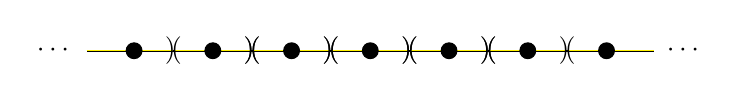
\begin{tikzpicture}
        \draw[step=1, black, thick] (-3.6, 0) -- (3.6, 0);
        \draw[yellow] (-3.6, 0) -- (-2.51, 0);
        \draw[yellow] (2.51, 0) -- (3.6, 0);
        \foreach \x in {-2, -1, 0, 1, 2} {
            \draw[yellow] (\x - 0.49, 0) -- (\x + 0.49, 0);
            \node at (\x - 0.5, 0) {$)\!($};
            \node at (\x + 0.5, 0) {$)\!($};
            \draw[fill=black] (\x, 0) circle (0.1);
        }
        \foreach \x in {-4, 4} {
            \node at (\x,0) {$\cdots$};
        }
        \draw[fill=black] (-3, 0) circle (0.1);
        \draw[fill=black] (3, 0) circle (0.1);
    \end{tikzpicture}
    \caption{The $\Z$ lattice packing in dimension $1$.}
    \label{Ch1:Fig:Z_Lattice_Packing_1D}
\end{figure}

In dimension $2$, \Cref{Ch1:Prob:SpherePacking_n}, also known as the circle packing problem, turns out to be more interesting. A reasonable strategy for finding the densest packing is to `stack' the $\Z$ lattice packing from dimension $1$ onto itself in some manner, turning these intervals into circles of the same radius. The question remains how to do this optimally.

One natural way of doing this is to stack the circles on top of themselves, turning $\Z$ into the lattice $\Z^2$, where circles are centred at points with integer coordinates: see \Cref{Ch1:Subfig:Z2_lattice_packing_2D}. Unfortunately, this packing turns out to be sub-optimal. A better candidate is the $A_2$ lattice packing: see \Cref{Ch1:Subfig:A2_lattice_packing_2D}. This packing is sometimes referred to as the \textit{honeycomb packing} due to the fact that every circle has six neighbours, whose centres form the vertices of a regular hexagon.

It is well-known that the honeycomb packing is optimal in $\R^2$. The original proof of this fact is attributed to Thue \cite{Thue}, but there are many proofs in the literature. One is outlined by Hales in \cite[p. 442]{CannonHoney}. An intuitive way of convincing oneself of Thue's theorem is that it is not possible for a circle in a given row to be in contact with more than $2$ circles in the rows above and below, meaning the $A_2$ packing cannot be improved. See \Cref{Ch1:Subfig:Kepler_Original_1}.

\begin{figure}[htb]
    \centering
    \begin{subfigure}{0.48\linewidth}
        \centering
        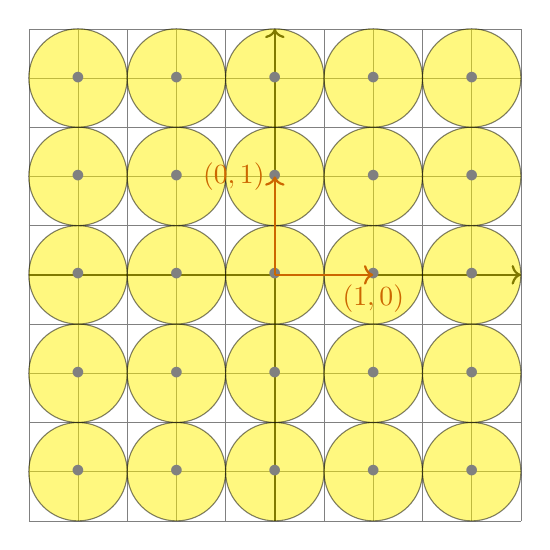
\begin{tikzpicture}[scale=1.25]
            \drawplane
            \foreach \x in {-2, -1, 0, 1, 2} {
                \foreach \y in {-2, -1, 0, 1, 2} {
                    \latticecircle{\x}{\y}
                }
            }
            \draw[->, color=brown, thick] (0,0) -- (1,0) node[anchor=north] {$\parenth{1, 0}$};
            \draw[->, color=brown, thick] (0,0) -- (0,1) node[anchor=east] {$\parenth{0, 1}$};
        \end{tikzpicture}
        \subcaption{The $\Z^2$ lattice packing.}
        \label{Ch1:Subfig:Z2_lattice_packing_2D}
    \end{subfigure}
    \begin{subfigure}{0.48\linewidth}
        \centering
        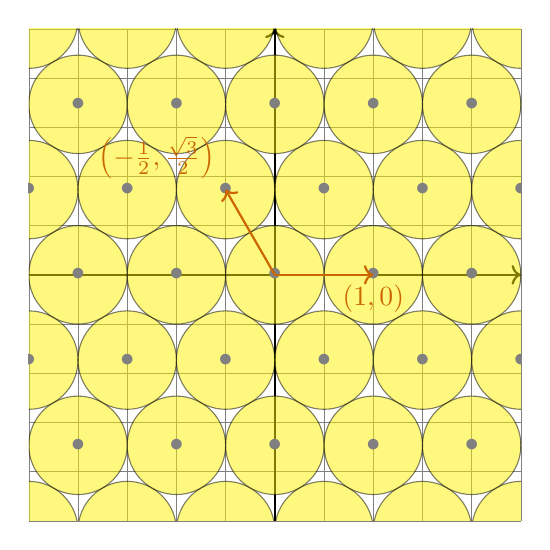
\begin{tikzpicture}[scale=1.25]
            \drawplane
            \clip (-2.5, -2.5) rectangle ++(5, 5);
            \foreach \x in {-4, -3, -2, -1, 0, 1, 2, 3, 4} {
                \foreach \y in {-3, -2, -1, 0, 1, 2, 3} {
                    \latticecircle{\x - \y * 0.5}{\y * 0.8660254038}
                }
            }
            \draw[->, color=brown, thick] (0,0) -- (1,0) node[anchor=north] {$\parenth{1, 0}$};
            \draw[->, color=brown, thick] (0,0) -- (-0.5,0.8660254038) node[anchor=south east] {$\parenth{-\frac{1}{2}, \frac{\sqrt{3}}{2}}$};
        \end{tikzpicture}
        \subcaption{The $A_2$ lattice packing.}
        \label{Ch1:Subfig:A2_lattice_packing_2D}
    \end{subfigure}
    \caption{Circle packings covering the square $\setst{\parenth{x, y} \subset \R^2}{-2.5 \leq x, y \leq 2.5}$.}
    \label{Ch1:Fig:Circle_Packings_2D}
\end{figure}

In dimension $3$, too, it is tempting to replicate this strategy: we can stack the $A_2$ packing on top of itself, in layers instead of rows, attempting to maximise the number of neighbours of a sphere. From trial and error, we see that a sphere cannot be in contact with more than three neighbours from the layer below. This suggests that the optimal sphere packing in dimension $3$ is given by stacking honeycomb arrangements on top of each other with spheres in each layer being nestled in the gaps between three spheres in the layer below.

\begin{wrapfigure}[28]{r}{0.27\linewidth}
    \centering
    \begin{subfigure}{\linewidth}
        \centering
        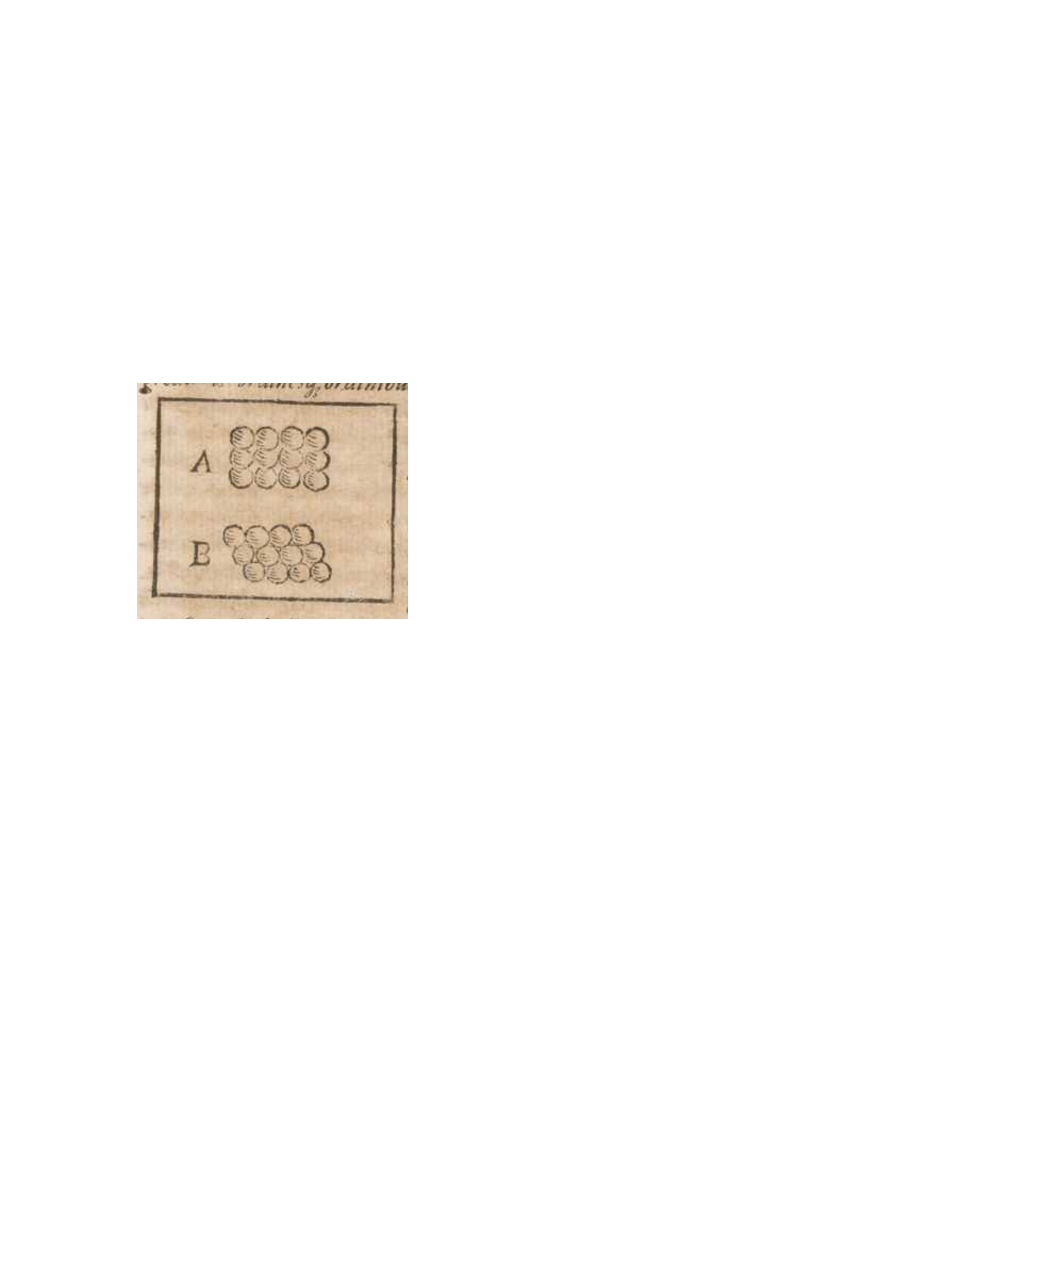
\includegraphics[width=\linewidth]{Chapters/1_Intro/Images/Kepler_1.pdf}
        \caption{}
        \label{Ch1:Subfig:Kepler_Original_1}
    \end{subfigure}
    \begin{subfigure}{\linewidth}
        \centering
        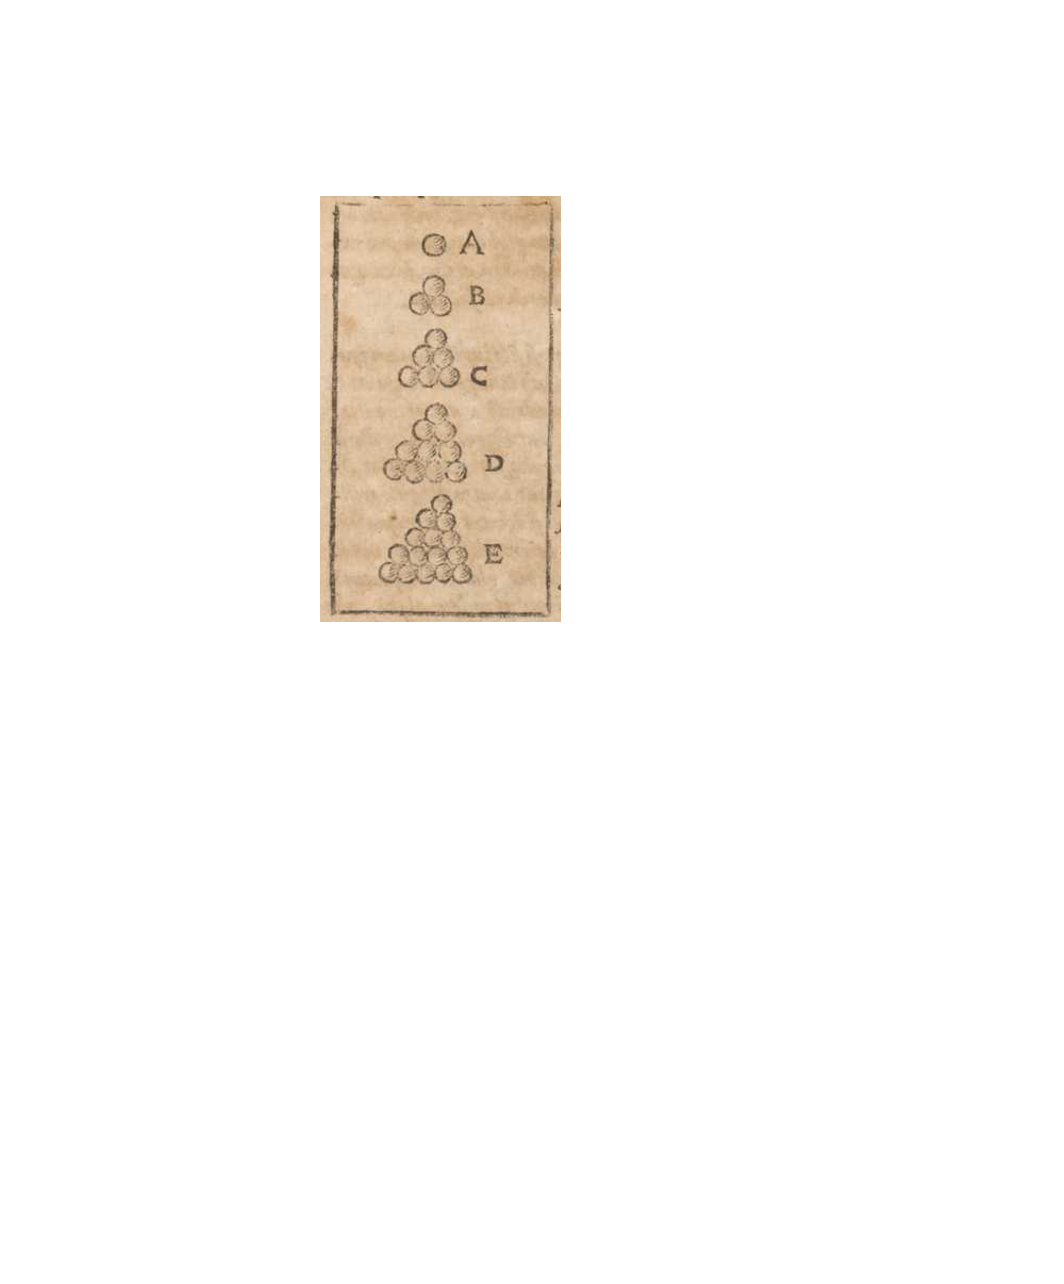
\includegraphics[width=\linewidth]{Chapters/1_Intro/Images/Kepler_2.pdf}
        \caption{}
        \label{Ch1:Subfig:Kepler_Original_2}
    \end{subfigure}
    \caption{Diagrams from an essay written by Johannes Kepler in Latin in 1611 \cite{KeplerSnowflake}.}
\end{wrapfigure}

As it turns out, unlike dimension $2$, this characterisation not describe a unique packing: spheres are simply too large! See \Cref{Ch1:Fig:2_Optimal_3D_Packings}. One can construct infinitely many locally similar, globally different sphere packings in $\R^3$, all of which are as dense as possible, by varying how successive layers are placed.

\begin{figure}[bt]
    \centering
    \begin{subfigure}{0.48\linewidth}
        \centering
        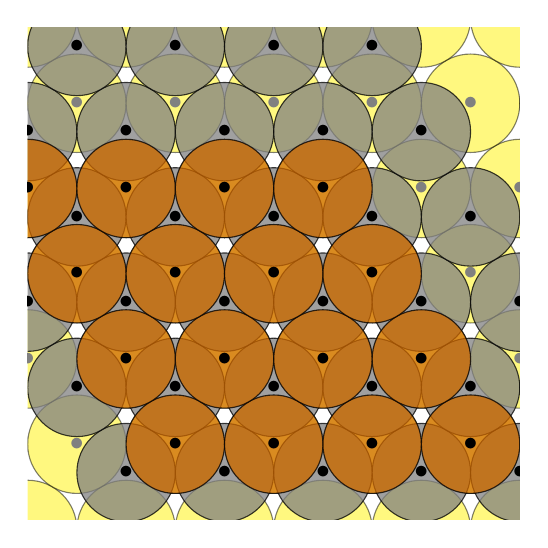
\begin{tikzpicture}[scale=1.25]
            \clip (-2.5, -2.5) rectangle ++(5, 5);
            \foreach \x in {-4, -3, -2, -1, 0, 1, 2, 3, 4} {
                \foreach \y in {-3, -2, -1, 0, 1, 2, 3} {
                    \latticecircle{\x - \y * 0.5}{\y * 0.8660254038}
                }
            }
            \foreach \x in {-3, -2, -1, 0, 1, 2} {
                \foreach \y in {-3, -2, -1, 0, 1, 2} {
                    \latticecirclegrey{\x - \y * 0.5}{\y * 0.8660254038 + 0.5773502692}
                }
            }
            \foreach \x in {-2, -1, 0, 1} {
                \foreach \y in {-2, -1, 0, 1} {
                    \latticecirclebrown{\x - \y * 0.5}{\y * 0.8660254038}
                }
            }
        \end{tikzpicture}
        \subcaption{}
        \label{Ch1:Subfig:3D_Triangular_Stacking}
    \end{subfigure}
    \begin{subfigure}{0.48\linewidth}
        \centering
        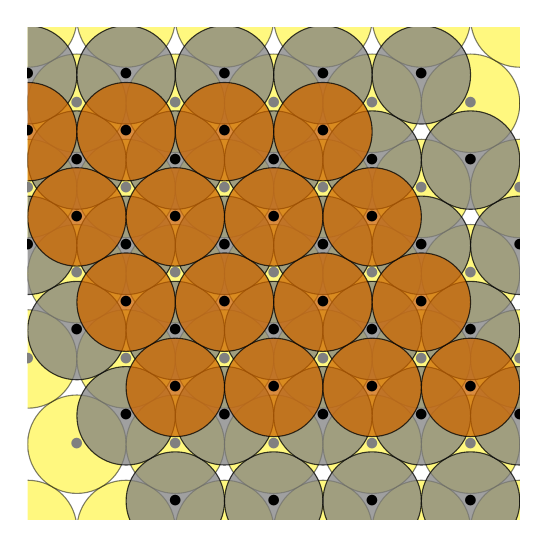
\begin{tikzpicture}[scale=1.25]
            \clip (-2.5, -2.5) rectangle ++(5, 5);
            \foreach \x in {-4, -3, -2, -1, 0, 1, 2, 3, 4} {
                \foreach \y in {-3, -2, -1, 0, 1, 2, 3} {
                    \latticecircle{\x - \y * 0.5}{\y * 0.8660254038}
                }
            }
            \foreach \x in {-2, -1, 0, 1, 2, 3} {
                \foreach \y in {-2, -1, 0, 1, 2, 3} {
                    \latticecirclegrey{\x - \y * 0.5}{\y * 0.8660254038 - 0.5773502692}
                }
            }
            \foreach \x in {-2, -1, 0, 1} {
                \foreach \y in {-2, -1, 0, 1} {
                    \latticecirclebrown{\x - \y * 0.5}{\y * 0.8660254038 + 0.5773502692}
                }
            }
        \end{tikzpicture}
        \subcaption{}
        \label{Ch1:Subfig:3D_Hexagonal_Stacking}
    \end{subfigure}
    \caption{Two different ways of stacking the honeycomb packing on itself.}
    \label{Ch1:Fig:2_Optimal_3D_Packings}
\end{figure}

This observation is not novel. In a 1611 essay whose title has been translated from Latin as \textit{The Six-Cornered Snowflake} \cite{KeplerSnowflake}, Johannes Kepler asserted that spheres cannot be more tightly packed together than they are in a tetrahedral arrangement: see \Cref{Ch1:Subfig:Kepler_Original_2}. This result became known as the Kepler Conjecture, and it went unproven for over three centuries, until 2005 that a paper proving it, written by Thomas Hales, was published \cite{HalesKeplerInformal}.

The complexity of the sphere packing problem in dimension $3$ is illustrated not only by the time elapsed between Kepler's original assertion and a proof being published but also by the length of Hales's paper. Indeed, in an expository account of his proof published in 2000, five years before the publication of the full paper in the Annals, Hales recounted how a jury of twelve referees, despite having been in deliberation for over a year, had yet to make a ``thorough, independent check of the computer code'' he had written to perform the elaborate calculations on which ``every aspect of [his proof] is based'' \cite{CannonHoney}. In January 2003, at the Joint Math Meetings in Baltimore, USA, Hales announced that he intended to formally verify his proof \cite{HalesKeplerFormal}, in what he termed the Flyspeck project. The paper authored by Hales and his collaborators on their successful formalisation of his argument was only published in 2017. Therefore, not only did the Kepler Conjecture take close to 400 years to solve, but it took nearly two decades to eliminate any doubt as to the correctness of the solution. This project aims to formalise a result of a similar flavour in a significantly shorter timeframe.
\section{The Work of Maryna Viazovska}
\section{The Formalisation Movement}
\section{Progress in Formalising Viazovska's Solution in Dimension $8$}

% Do I want to turn this into a separate chapter and toss in section 1.5?
\section{The Scope of this Project}
\chapter{The Ingredients of Viazovska's Solution}
\thispagestyle{empty}
% It might be worth chucking a large part of this chapter into an appendix. Specifically, §2.1.1 (Sphere Packing Fundamentals) and §2.3 (Modular Forms). Need to think about this... this would also depend on how we phrase §1.3 (scope of project) because we need to make it EXTREMELY CLEAR that the purpose of this project was NOT to delve deep into a cool application of the theory of modular forms but rather to learn how to formalise modern, computationally involved mathematics.

The purpose of this chapter is to offer background information that will be essential to understanding the rest of this exposition. We will begin by providing precise mathematical definitions for sphere packings, densities, and the sphere packing constant. We will then discuss the variation of the linear programming bound proven by Cohn and Elkies \cite[Theorem 3.1]{CohnElkies} used by Viazovska \cite[Theorem 2]{Viazovska8}. Finally, we will include a small discussion on the theory of modular forms and establish its relevance to the subsequent chapters of this thesis, which will focus on the construction of the Magic Function.

We will be minimalistic in our discussions, and focus on motivating new concepts and their relevance to the sphere packing problem in dimension $8$. This section is not intended to offer an exhaustive treatment of the mathematics we will encounter, which is as vast as it is rich.

\section{Preliminaries}

Before we begin defining things formally, we must include a small disclaimer about the terminology we have been using---and will continue to use---in this project. While \Cref{Ch1:Prob:SpherePacking_n} is usually referred to as the \textit{sphere} packing problem, a sphere is not usually thought to have an interior. Typically, in any metric space $X$ with metric $d$, the \textit{sphere} of radius $r \geq 0$ centred at $x \in X$ is defined to be $\setst{y \in X}{d(x, y) = r}$. In other words, the sphere consists only of a surface. In contrast, the sphere packing problem involves packing \textit{solid balls}. One can see why, in \cite{CannonHoney}, Hales opines that a more proper term for the problem would be the \textit{ball packing problem}. Nevertheless, in this project, we will continue to use the standard terminology, but we include this disclaimer so the reader bears in mind two things: first, that we will often mean `ball' when we use the word `sphere', and second, that we work with balls instead of spheres in Lean. We will also mention that it is convenient to require that the balls in question be open, so that the condition that spheres cannot overlap but merely touch tangentially can be shortened to that of disjointedness. We introduce notation.

\begin{boxnotation}
    For some $d \in \N$, $x \in \R^d$ and $r > 0$, we denote
    \begin{align*}
        B_d(x, r) := \setst{y \in \R^d}{\norm{x - y} < r}
    \end{align*}
\end{boxnotation}

We organise this section into three subsections. The first defines fundamental notions about sphere packings. The second introduces the properties of two important, and closely related, classes of sphere packings, namely, lattice packings and periodic packings. The third subsection studies the most important sphere packing for our project: the $E_8$ lattice packing.

\subsection{Sphere Packing Fundamentals}

We begin by defining a sphere packing. As we have stated, we want sphere packings to consist of disjoint spheres of the same radius. Given that lying on the interior of a certain sphere corresponds to being within some distance from its centre, we can capture this notion of disjointedness by imposing a separation condition on the set of centres of the sphere packing.

\begin{boxdefinition}[Sphere Packing]
    Fix $d \in \N$ and $X \subset \R^d$. Assume that there exists a real number $r > 0$, known as the \textbf{separation radius}, such that
    \begin{align*}
        \norm{x - y} \geq r
    \end{align*}
    for all distinct $x, y \in X$. We define the \textbf{sphere packing with centres at $X$} to be
    \begin{align*}
        \Pa(X) := \bigcup_{x \in X} B_d(x, r)
    \end{align*}
\end{boxdefinition}

Note that the assumption that a separation radius exists is very important.

\begin{boxnexample}
    Let $d = 1$ and $X = \R$. Consider the set
    \begin{align*}
        \bigcup_{x \in \R} B_1(x, r) = \bigcup_{x \in \R} \parenth{x-r, x+r}
    \end{align*}
    For any $r > 0$, the above union is all of $\R$. However, it does not make sense to construct a sphere packing whose set of centres is the entirety of $\R$, as this would involve spheres overlapping. It is precisely to avoid such constructions that we impose the condition that $r$ be a separation radius on the set of centres.
\end{boxnexample}

Since all the information about a sphere packing is encoded in its set of centres and the corresponding separation radius (which must exist in order for the set of centres to be a valid set of centres for a sphere packing), we decided that a sphere packing would be formalised purely as a set of centres with a valid separation, and that a separate definition would be made to obtain the open balls that constitute the packing. We packaged the data of
\begin{itemize}
    \item the set of centres
    \item the separation radius
    \item the (automatically checked) condition that the separation radius is positive
    \item the condition that the set of centres is, indeed, separated by this radius
\end{itemize}
into a \verb|structure| called \verb|SpherePacking|: see \cite[\texttt{SpherePacking.Basic.SpherePacking}]{documentation}.\todo{Is this an acceptable way of citing the documentation? Should the repo be made public?}

We now define finite density, an indicator of how much of a bounded region of space a sphere packing covers.

\begin{boxdefinition}[Finite Density]\label{Ch2:Def:FiniteDensity}
    Let $\Pa$ be a sphere packing. For all $R > 0$, define the \textbf{finite density} to be
    \begin{align*}
        \Delta_\Pa(R) := \frac{\Volof{\Pa \cap B_d(0, R)}}{\Volof{B_d(0, R)}}
    \end{align*}
    where $\Vol$ is the Lebesgue measure on $\R^d$.
\end{boxdefinition}

Finite density is a somewhat local notion, in that it expresses sphere how closely packed spheres are in a bounded region. The sphere packing problem, on the other hand, examines the notion of closeness on a more global level. While taking the limit of finite densities as the radius of the bounding region approaches infinity might seem like a natural way to define density, it is not obvious that this limit always exists. Therefore, we define density to be the limit superior instead.

\begin{boxdefinition}[Density]\label{Ch2:Def:Density}
    Let $\Pa$ be a sphere packing. Define the \textbf{density} of $\Pa$ to be
    \begin{align*}
        \Delta(\Pa) := \limsup_{R \to \infty} \Delta_\Pa(R)
    \end{align*}
    where $\Delta_\Pa(R)$ is the finite density of $\Pa$, as defined in \Cref{Ch2:Def:FiniteDensity}.
\end{boxdefinition}

As one might expect, finite density and density are invariant under scaling.

\begin{boxproposition}\label{Ch2:Prop:Scaling_Sphere_Packings}
    Let $\Pa$ be a sphere packing. Fix $\lambda > 0$. Denoting by $\lambda \Pa$ the sphere packing obtained by scaling the spheres and the set of centres in $\Pa$ by a factor of $\lambda$, we have
    \begin{align*}
        \Delta_{\Pa}\of{R} = \Delta_{\lambda \Pa}\of{\lambda R}
    \end{align*}
    for all $R > 0$. Similarly, we have
    \begin{align*}
        \Delta\of{\Pa} = \Delta\of{\lambda \Pa}
    \end{align*}
\end{boxproposition}

The sphere packing problem asks for the sphere packing that achieves the highest possible density. We can be formal about the notion of the highest possible density.

\begin{boxdefinition}[Sphere Packing Constant]
    The \textbf{sphere packing constant} in $\R^d$, for any $d > 0$, is defined to be
    \begin{align*}
        \Delta_d := \sup\!\parenth{{\setst{\Delta_{\Pa}}{\Pa \text{ is a sphere packing in } \R^d}}}
    \end{align*}
\end{boxdefinition}

\Cref{Ch2:Prop:Scaling_Sphere_Packings} tells us that it suffices to take the supremum over sphere packings of separation $1$, because a sphere packing $\Pa$ can be scaled down by its separation radius to obtain a sphere packing of separation $1$.

\begin{boxproposition}\label{Ch2:Prop:Scaling_Sphere_Packing_Constant}
    For all $d$, we have
    \begin{align*}
        \Delta_d = \sup\!\parenth{{\setst{\Delta_{\Pa}}{\Pa \text{ is a sphere packing in } \R^d \text{ with separation } 1}}}
    \end{align*}
\end{boxproposition}

As intuitive as this result might seem, we do mention it here because it is something we have to deal with explicitly when formalising the theory of sphere packings in Lean. The first instance when we really see it in action is the proof of \Cref{SP:Thm:CohnElkies}.

The objective of the sphere packing problem in any dimension $d$ is to optimise the sphere packing constant $\Delta_d$. As we have seen, this is a highly non-trivial thing to do. We can, however, offer a trivial upper-bound on sphere packing density.

\begin{boxlemma}
    For any sphere packing $\Pa$ and $R > 0$, we have that $\Delta_{\Pa}(R) \leq 1$.
\end{boxlemma}
\begin{proof}
    This is an immediate consequence of the fact that $\Pa \cap B_d(0, R) \subseteq B_d(0, R)$.
\end{proof}
This immediately gives us the following basic facts.
\begin{boxcorollary}
    For any sphere packing $\Pa$, we have that $\Delta_{\Pa} \leq 1$.
\end{boxcorollary}
\begin{boxcorollary}
    For any $d \in \N$, $\Delta_d \leq 1$.
\end{boxcorollary}

This is not a very good upper-bound. However, it tells us that the sphere packing constant in any number of dimensions is a finite real number in the interval $(0, 1]$. There is still some work to be done before we can give better bounds on the sphere packing constant. Furthermore, it is unclear whether the sphere packing constant actually is, for a general $d$, the density of a sphere packing in $\R^d$. Nevertheless, this is a good starting point.

A great deal of basic sphere packing API in Lean was developed in July 2024 for the project to formalise Viazovska's solution in dimensino $8$. The majority of the code was written by Gareth Ma, who also made significant improvements to the design choices I had made when setting up the project. The definitions and results in this section have all been formalised, and information about the code that has been written can be found in the project documentation \cite[\texttt{SpherePacking.Basic.SpherePacking}]{documentation}.

In the next subsection, we discuss a special class of sphere packings that have periodicity properties with respect to lattices.

\subsection{Lattice and Periodic Sphere Packings}

We begin by defining lattices and briefly commenting on existing \verb|Mathlib| API on lattices. There are primarily two ways in which lattices are defined in mathematical literature. A lattice in some Euclidean space $\R^n$ is either described as the $\Z$-span of some $\R$-basis of $\R^n$ or as a discrete, co-compact subgroup. One can borrow characteristics from both definitions to construct other equivalent definitions.

The characteristics described in both definitions do exist \verb|Mathlib|. However, given that one of the objectives of creating a unified mathematics library is centralisation, a combination of these definitions is used as the \textit{definition} of a \verb|class| that we call \verb|IsZLattice| and information about its many properties, as well as the $\Z$-span construction, are encoded in theorems. In particular, we have a theorem that tell us that every lattice is a free $\Z$-submodule, meaning it has a $\Z$-basis, and that this $\Z$-basis is actually an $\R$-basis of the ambient space. Furthermore, we have a result that every object constructed in that manner is a lattice. Results about types bearing the \verb|IsZLattice| class (ie, lattices as they are defined in \verb|Mathlib|) live in the \verb|ZLattice| namespace, whereas results bout $\Z$-spans of $\R$-bases live in the \verb|ZSpan| namespace. \todo{Create citation for Mathlib.}

We begin by stating the \verb|Mathlib| definition of a lattice.

\begin{boxdefinition}[Lattice]
    A \textbf{lattice} in a Euclidean space $\R^n$ is a discrete $\Z$-submodule of $\R^n$ such that its $\R$-span contains every element in $\R^n$.
\end{boxdefinition}

The \verb|Mathlib| definition is more general, and works for any normed vector space over a normed field. Here, the word `discrete' means that the lattice is discrete in a topological sense, meaning that the subspace topology on the lattice is precisely the discrete topology.

\begin{boxdefinition}[Periodic Sphere Packing]
    Let $\Lambda \subset \R^d$ be a lattice. We say a sphere packing $\Pa(X)$ with spheres centred at points in $X \subset \R^d$ is \textbf{periodic with respect to $\Lambda$}, or \textbf{$\Lambda$-periodic},
    \begin{align*}
        \lambda + X = X
    \end{align*}
    ie, for all $\lambda \in \Lambda$ and $x \in X$, we have that $\lambda + x \in X$.
\end{boxdefinition}

We define Periodic Sphere Packings in Lean as extending the definition of Sphere Packings by creating a \verb|structure| called \verb|PeriodicSpherePacking| that packages the additional data of
\begin{itemize}
    \item the lattice, viewed as a $\Z$-submodule of the ambient space $\R^d$
    \item the condition that the set of centres is periodic with respect to this $\Z$-submodule
    \item the (automatically checked) condition\footnotemark{} that the $\Z$-submodule is discrete
    \item the (automatically checked) condition\footnotemark[\value{footnote}] that the discrete $\Z$-submodule is a lattice
\end{itemize}
\footnotetext{more precisely, the automatically inferred instance}
The definition is in \cite[\texttt{SpherePacking.Basic.SpherePacking}]{documentation}.

Lattice packings are a special class of periodic packings.

\begin{boxdefinition}[Lattice Packing]
    Let $\Lambda \subset \R^d$ be a lattice. The \textbf{$\Lambda$ lattice packing} is the sphere packing with centres at points in $\Lambda$. Such a sphere packing admits a separation radius because $\Lambda$ is discrete and is $\Lambda$-periodic because $\Lambda$ is closed under addition.
\end{boxdefinition}

In \Cref{Ch2:Subsec:E8}, we will briefly examine a specific lattice packing, the $E_8$ lattice packing.

The periodicity property of a periodic sphere packing can be exploited to derive a more convenient formula for its density.

\begin{boxproposition}\label{Ch2:Prop:Periodic_Density}
    Let $\Pa(X)$ be a sphere packing with centres at $X \subset \R^d$ and separation $r$ that is periodic with respect to some lattice $\Lambda \subset \R^d$. We have that
    \begin{align}
        \Delta_{\Pa(X)} = \abs{\quotient{X}{\Lambda}} \frac{\Volof{B_d\of{0, \frac{r}{2}}}}{\Volof{\quotient{\R^d}{\Lambda}}}
        \label{Ch2:Eq:Periodic_Density}
    \end{align}
\end{boxproposition}

The proof is beyond the scope of this M4R project, but was formalised in Summer 2024: see \verb|PeriodicSpherePacking.density_eq'| in \cite[\texttt{SpherePacking.Basic.PeriodicPacking}]{documentation}.

Just as we defined the sphere packing constant for any dimension $d \in \N$, we can define a \textit{periodic} sphere packing constant in any dimension.

\begin{boxdefinition}[Periodic Sphere Packing Constant]
    For all $d \in \N$, define the \textbf{periodic sphere packing constant in dimension $d$} to be
    \begin{align*}
        \Delta_{d}^{\periodic} = \sup\of{{\setst{\Delta_{\Pa}}{\Pa \text{ is a periodic sphere packing in } \R^d}}}
    \end{align*}
\end{boxdefinition}

The power of periodic sphere packings is illustrated by a rather surprising fact.

\begin{boxproposition}\label{Ch2:Prop:Periodic_Const_eq_Const}
    For all $d \in \N$,
    \begin{align*}
        \Delta_{d} = \Delta_{d}^{\periodic}
    \end{align*}
\end{boxproposition}

We do not prove this result here, as it is beyond the scope of this M4R. A proof can be found in \cite[Appendix A]{CohnElkies}. We do, however, mention that \Cref{Ch2:Prop:Periodic_Const_eq_Const} can be combined with \Cref{Ch2:Prop:Scaling_Sphere_Packing_Constant} to give the following.

\begin{boxproposition}\label{Ch2:Prop:Scaling_Periodic_Constant}
    For all $d \in \N$,
    \begin{align*}
        \Delta_{d} = \sup\of{{\setst{\Delta_{\Pa}}{\Pa \text{ is a periodic sphere packing in } \R^d \text{ with separation } 1}}}
    \end{align*}
\end{boxproposition}

\Cref{Ch2:Prop:Periodic_Const_eq_Const} tells us that finding a sphere packing that satisfies the \textit{periodic} sphere packing constant gives us the optimal sphere packing in dimension $d$. \Cref{Ch2:Prop:Scaling_Periodic_Constant} allows us to focus our search even more. We will exploit these two facts in \Cref{Ch2:Sec:CohnElkies}, where we will construct an upper bound for all sphere packing densities in dimension $d$ by constructing an upper-bound for the periodic sphere packing constant in dimension $d$. When constructing this upper-bound, we will exploit the fact that periodic sphere packings admit a `nice' density formula (cf. \Cref{Ch2:Prop:Periodic_Density}). The results we have seen about periodic sphere packings will thus greatly simplify our task of finding the optimal sphere packing in dimension $8$.

We are now ready to discuss a special sphere packing in $\R^8$: the $E_8$ sphere packing.

\subsection{The $E_8$ Lattice Packing}\label{Ch2:Subsec:E8}

\begin{wrapfigure}[18]{r}{0.5\linewidth}
    \vspace{-3em}
    \centering
    \includegraphics[width=0.98\linewidth]{Chapters/2_Dimension_8/Images/Gorbe_E8.png}
    \caption{The Coxeter projection of the $E_8$ root system. \cite{Gorbe_E8}}
    \label{Ch2:Fig:Gorbe_E8}
\end{wrapfigure}

It is quite remarkable that $E_8$ should show up when discussing sphere packings. At its core, $E_8$ is an irreducible root system. It shows up in the classification of important classes of objects like irreducible Coxeter groups, crystallographic Coxeter groups, and semi-simple Lie algebras over $\C$. $E_8$ is not a classical root system but an \textit{exceptional} root system, meaning that the geometric properties of its roots cannot be found in irreducible root systems in all dimensions.

The $E_8$ root system consists of $240$ vectors in $\R^8$ that are permuted by a certain finite subgroup of the $8$-dimensional orthogonal group. This group is sometimes referred to as the $E_8$ Coxeter group or as the Weyl group of the $E_8$ lattice. These roots can be divided into $8$ orbits, each of which corresponds to one of the `layers' of concentric circles in \Cref{Ch2:Fig:Gorbe_E8}. The dots in the figure correspond to projections of the roots onto a plane on which a specific type of element of the Coxeter group, known as a Coxeter element, acts as a rotation. This visualisation offers a convenient---and aesthetically pleasing---means of visualising this collection of $8$-dimensional vectors and appreciating some of its symmetry.

% From a motivational standpoint, this is quite important. So mention facts like distances between lattice points and things like that. Important for construction of magic function.



\section{The Cohn-Elkies Linear Programming Bounds}
\section{A Word on Modular Forms}
\label{Ch2:Sec:ModForms}
% SHOULD I MAYBE TURN THIS INTO AN APPENDIX? IT'S LOOKING PRETTY LONG...

\begin{comment}
Things to discuss:
1. What is a modular form
2. What is a quasimodular form
3. Examples: Eisenstein Series, Jacobi Theta functions, Discriminant form
We can reference things like the q-expansions of the Eisenstein series, the transformation rules for the Jacobi theta functions, and the product formula for the discriminant form.
\end{comment}

In this section, we give a brief introduction to the theory of modular forms. Birkbeck, Loeffler and others have formalised several results in the theory of modular forms, and a significant portion of their work has been merged into \mathlib. Definitions and results from this section that pertain to Viazovska's solution to the sphere packing problem in $\R^8$ that do not feature in \mathlib\ are being actively formalised by Birkbeck and Lee, with contributions from Ma.

First, we introduce the following useful notation.

\begin{boxnotation}
    For the remainder of this paper, denote the Complex upper half-plane by $\Halfplane$. That is, define $\Halfplane := \setst{z \in \C}{0 < \Im(z)}$.
\end{boxnotation}

This corresponds to the \mathlib\ notation for the upper half-plane.

A key motivating idea in the study of modular forms is the study of the action of $\SL{2, \Z}$ on $\Halfplane$ by Möbius transformations via
\begin{align*}
    \begin{bmatrix}
        a & b \\ c & d
    \end{bmatrix}
    \cdot z := \frac{az + b}{cz + d}
\end{align*}
That matrix multiplication corresponds to the composition of Möbius transformations is a well-known fact in Complex Analysis. One can hence show that the above is indeed a group action.

Both the identity $I \in \SL{2, \Z}$ and the negative identity $-I \in \SL{2, \Z}$ have the same (trivial) action on $\Halfplane$. Indeed, the $\SL{2, \Z}$ action descends to a faithful action of $\PSL{2, \Z} = \quotient{\SL{2, \Z}}{\set{\pm I}}$ on $\Halfplane$. Since we are more interested in the \textit{actions} of matrices in $\SL{2, \Z}$ and $\PSL{2, \Z}$ than we are in their entries, we often do not distinguish between the two groups.

The \mathlib\ definition of a modular form is more general than the first definitions of modular forms often seen in literature (see \cite[Chapter VII, \S 2, Definition 4]{SerreArith} and \cite[Definition 1.1.2]{DiamondShurman}), and instead matches subsequent definitions that generalise these first definitions. Modular forms are usually described as functions that are holomorphic on the upper half-plane that are invariant under the $\SL{2, \Z}$-action up to an \textit{automorphy factor} of a certain \textit{weight}. This \textit{weight} is defined as the \textit{weight of the modular form}. However, one is often interested in invariance under not all of $\SL{2, \Z}$, but certain \textit{principal congruence subgroups} or subgroups containing such subgroups, known as \textit{congruence subgroups}. Each principal congruence subgroup has a \textit{level}, which is defined to be the \textit{level} of a modular form whose congruence subgroup is principal. Modular forms, as they are defined in \mathlib\ and in the blueprint \cite{blueprint}, are therefore indexed by two properties: a \textit{congruence subgroup of $\SL{2, \Z}$}, which indicates the scope of invariance under the $\SL{2, \Z}$-action, and a \textit{weight}, which gives the extent of invariance under the action of elements of the subgroup in question.

To give a complete definition of the weight of a modular form, we need to define automorphy factors and the slash action notation.

\begin{boxdefinition}[Automorphy Factors and Slash Actions]\label{Ch2:Def:Aut_Factor_Slash_Action}
    Fix $k \in \Z$, $z \in \Halfplane$ and $\gamma = \begin{bmatrix} a & b \\ c & d \end{bmatrix} \in \SL{2, \Z}$. Define the \textbf{automorphy factor of weight $k$} to be
    \begin{align}
        j_k\of{z, \gamma} &:= \parenth{cz + d}^{-k}
        \label{Ch2:Eq:AutomorphyFactor_def}
    \end{align}
    For any function $f : \Halfplane \to \C$, with $k$ and $\gamma$ as above, the \textbf{slash operator} maps $f$ to a new function $f \mid_k \gamma : \Halfplane \to \C$ given by
    \begin{align}
        \fmof{k}{\gamma}{z} &:= j_k\of{z, \gamma} \fof{\gamma \cdot z} = \parenth{cz + d}^{-k} \fof{\frac{az + b}{cz + d}}
        \label{Ch2:Eq:SlashAction_def}
    \end{align}
    The action of $\gamma$ mapping $f$ to $\fm_k \gamma$ via the weight $k$ slash operator is sometimes referred to as a \textbf{slash action}.
\end{boxdefinition}

It is clear, from the above definition, that $\fm_0 \gamma = f \circ \gamma$ for al $\gamma \in \SL{2, \Z}$. That is, if $f = \fm_0 \gamma$, then $f = f \circ \gamma$, that is, $f$ is invariant under composition with (the action of) $\gamma$. If $f = \fm_k \gamma$ for some $k \in \Z$ and $\gamma \in \SL{2, \Z}$, we can view the weight $k$ as indicating the `extent of invariance' of $f$ under composition with $\gamma$. Note that slash actions can be composed.

\begin{boxlemma}\label{Ch2:Lemma:Slash_Mul}
    For all $k \in \Z$, $f : \Halfplane \to \C$ and $\gamma_1, \gamma_2 \in \SL{2, \Z}$,
    \begin{align*}
        \parenth{f \mid_k \gamma_1} \mid_k \gamma_2 = f \mid_k \parenth{\gamma_1 \gamma_2}
    \end{align*}
    where $\gamma_1 \gamma_2$ is the product of $\gamma_1$ and $\gamma_2$ as matrices.
\end{boxlemma}
A slightly more general version of this has been \href{https://github.com/leanprover-community/mathlib4/blob/a0370507e2922f0a329a2d8cc17e9f9148cd168d/Mathlib/NumberTheory/ModularForms/SlashActions.lean#L77}{formalised} in \mathlib.

We are now ready to define congruence subgroups, which will tell us under precisely which elements of $\SL{2, \Z}$ a modular form is slash-invariant. We express this notion in the language of modular arithmetic.

\begin{boxdefinition}[Congruence Subgroup]\label{Ch2:Def:Cong_Subgroup}
    Fix $N \in \N$. The \textbf{level $N$ principal congruence subgroup} of $\SL{2, \Z}$, denoted $\Gamma(N)$, is defined to be the kernel of the surjective group homomorphism from $\SL{2, \Z}$ to $\SL{2, \Zmod{N}}$ that comes from reducing modulo $N$. That is,
    \begin{align}
        \Gamma(N) &:= \setst{
        \begin{bmatrix}
            a & b \\ c & d
        \end{bmatrix} \in \SL{2, \Z}}{
        \begin{bmatrix}
            a & b \\ c & d
        \end{bmatrix}
        \equiv
        \begin{bmatrix}
            1 & 0 \\ 0 & 1
        \end{bmatrix}
        \pmod{N}}
        \label{Ch2:Eq:PrincipalCongruenceSubgroup_def}
    \end{align}
    More generally, a subgroup $\Gamma$ of $\SL{2, \Z}$ is called a \textbf{congruence subgroup} if $\Gamma(N) \subset \Gamma$ for some $N \in \N$.
\end{boxdefinition}

We now have enough to define what it means for a holomorphic function to be invariant under the slash action of a congruence subgroup. In the definition of modular forms, however, we include an additional condition that is often referred to as \textit{holomorphicity at $i\infty$}, the purpose of which is to ensure that spaces of modular forms, which turn out to admit $\C$-vector space structures, are, in fact, finite-dimensional \cite{KevinFamilies}.

The theory of modular forms is often thought to lie in the very rich intersection of algebra and analysis. Our definitions so far have been largely algebraic, but our next one is analytic. Consider the mapping $q : \Halfplane \to \C : z \mapsto e^{2\pi i z}$. This maps $\Halfplane$ to the punctured, open unit disc
\begin{align*}
    D := \setst{w \in \C}{0 < \abs{q} < 1}
\end{align*}
Indeed, for all $z \in \Halfplane$, writing $z = x + iy$ for $x, y \in \R$ with $y > 0$, we have
\begin{align*}
    \abs{q(z)} = \abs{e^{2 \pi i \parenth{x + iy}}} = \abs{e^{2\pi i x}} \cdot \abs{e^{-2\pi y}} < 1
\end{align*}
with $0 \notin q\of{\Halfplane}$ but $q(z) \to 0$ as $\Im(z) = y \to \infty$. Now, we know that the holomorphic functions from $D \to \C$ are precisely those that have Laurent expansions of the form
\begin{align*}
    \sum_{n=0}^{\infty} c_n w^n
\end{align*}
for all $w \in D$. If we write $w = q(z)$ for $z \in \Halfplane$, the above series turns out to be a \textit{Fourier expansion}. We can hence make the following definition for holomorphicity at $i\infty$.

\begin{boxdefinition}[Holomorphicity at $i\infty$]\label{Ch2:Def:Holo_at_ImInfty}
    We say a function $f : \Halfplane \to \C$ is \textbf{holomorphic at $i\infty$} if $f$ admits a Fourier expansion of the form
    \begin{align*}
        f(z) = \sum_{n=0}^{\infty} c_n q(z)^n = \sum_{n=0}^{\infty} c_n e^{2\pi i nz}
    \end{align*}
    That is, $f$ admits a Fourier expansion with no negative powers of $q(z)$.
\end{boxdefinition}

The holomorphicity of $f$ at $i\infty$ essentially means that the Fourier expansion of $f$ is a holomorphic $D \to \C$ function in $q(z)$, with the added constraint that $\abs{f(z)}$ remains bounded as $\Im(z) \to \infty$, that is, the corresponding $D \to \C$ function in $q(z)$ extends to a holomorphic function that is defined and bounded at $0$. There is a rich theory of functions where $c_0 = 0$, but we will not explore that theory here.\footnote{Modular forms with this property are known as \textbf{cusp forms}. One modular form we will need to construct the magic function is the discriminant form, which will turn out to be a cusp form.}

We are now ready to define modular forms. Intuitively, a modular form is a function that satisfies the above definitions in a slash-invariant manner. More precisely, we have the following.

\begin{boxdefinition}[Modular Form]
    Fix $k \in \Z$ and let $\Gamma$ be a congruence subgroup of $\SL{2, \Z}$. We say a function $f : \Halfplane \to \C$ is a \textbf{modular form of weight $k$ with respect to $\Gamma$} if $f$ is \textbf{invariant} under the slash action of $\Gamma$ and \textbf{holomorphic at $i\infty$} under the slash action of $\SL{2, \Z}$. That is,
    \begin{enumerate}
        \item For all $\gamma \in \Gamma$, $\fm_k \gamma = f$ (cf. \Cref{Ch2:Def:Aut_Factor_Slash_Action}).
        \item For all $\gamma \in \SL{2, \Z}$, $\fm_k \gamma$ is holomorphic at $i\infty$ (cf. \Cref{Ch2:Def:Holo_at_ImInfty}).
    \end{enumerate}
    We denote by $M_k(\Gamma)$ the space of modular forms of weight $k$ and congruence subgroup $\Gamma$. If $\Gamma = \Gamma(N)$ for some $N \in \N$, we say an element of $M_k(\Gamma)$ has \textbf{level $N$}.
\end{boxdefinition}

There is an immensely rich theory of modular forms, and for the purposes of practicality, it was decided not to explore this theory in great detail in this project, particularly because the formalisation of the aspects of Viazovska's proof that stem from this theory is being led by Birkbeck, Lee and Ma. We will instead use the remainder of this section to discuss three specific (families of) modular forms and those of their properties that Viazovska uses to construct her magic function.

\subsection{The Eisenstein Series}
\label{Ch2:Subsec:EisensteinSeries}

The Eisenstein Series are an important family of slash-invariant forms that will prove essential to the construction of the magic function. The Eisenstein Series whose \textit{weight} is an even integer that is at least $4$ are modular forms, though we will also need to work with the Eisenstein Series of weight $2$, which, despite not being a modular form, is sufficiently well-behaved for our purposes. We will define it separately from those Eisenstein Series that are modular forms.

Let $k \geq 4$ be an even integer. We denote by $E_k$ the weight $k$ Eisenstein Series. There is more than one way to define $E_k$. In this report, we give the definition that was formalised by Birkbeck for this project. Birkbeck's definition in the project repository is a particular case of the \href{https://github.com/leanprover-community/mathlib4/blob/70816aec3a0f7bb98ac42991652a66b6405e1a00/Mathlib/NumberTheory/ModularForms/EisensteinSeries/Basic.lean#L28-L35}{\mathlib\ definition}, which defines it as a \texttt{ModularForm} structure combining the function \href{https://github.com/leanprover-community/mathlib4/blob/70816aec3a0f7bb98ac42991652a66b6405e1a00/Mathlib/NumberTheory/ModularForms/EisensteinSeries/Defs.lean#L107}{\texttt{eisensteinSeries}} with the proofs of the properties that make it a modular form. The \mathlib\ definition is more general than the one we study here, and involves imposing congruence conditions on the subsets of the lattice $\Z^2$ over which the Eisenstein Series are summed. It is not necessary for this project.

\begin{boxdefinition}[The Eisenstein Series of Even Weight $\geq 4$]\label{Ch2:Def:EisensteinSeries_geq_4}
    For $k \geq 4$ even, define the \textbf{weight $k$ Eisenstein Series} to be the function $E_k : \Halfplane \to \C$ given by
    \begin{align}
        E_k(z) := \frac{1}{2} \sum_{\substack{\parenth{m, n} \in \Z^2 \\ \gcd(m, n) = 1}} \frac{1}{\parenth{mz + n}^k}
        \label{Ch2:Eq:Eisenstein_def_Chris}
    \end{align}
    with the defining summation converging absolutely.
\end{boxdefinition}

Note that the Eisenstein Series can also be defined as
\begin{align}
    E_k(z) = \frac{1}{2\zeta(k)} \sum_{\parenth{m, n} \in \Z^2 \setminus \set{0}} \frac{1}{\parenth{mz + n}^k}
    \label{Ch2:Eq:Eisenstein_def_with_zeta_normalisation}
\end{align}
with $\zeta$ here denoting the Riemann zeta function. It is shown in \cite[Equation (4.1), pp. 109-110]{DiamondShurman} that this definition matches the definition formalised by Birkbeck in the project repository and stated informally in \Cref{Ch2:Def:EisensteinSeries_geq_4}.\todo{Blueprint gives zeta def whereas repo gives coprime def. WHOOPSIE!}

It is shown in \cite[pp. 4-5]{DiamondShurman} that $E_k$ is a weight $k$, level $1$ modular form for even integers $k \geq 4$. That is, $E_k$ is invariant under the weight $k$ slash-action of every element of $\SL{2, \Z}$. As important special cases of this, $E_k$ satisfies two important functional equations.

\begin{boxproposition}\label{Ch2:Prop:Eisenstein_func_eq}
    For all even $k \geq 4$ and $z \in \Halfplane$, the following both hold:
    \begin{align}
        E_k\of{z + 1} &= E_k \label{Ch2:Eq:Ek_func_eq_one_add} \\
        E_k\of{-\frac{1}{z}} &= z^k E_k(z) \label{Ch2:Eq:Ek_func_eq_neg_one_div}
    \end{align}
\end{boxproposition}
\begin{proof}
    Both of these are just slash-invariance properties in disguise. We have\todo{Fix slash formatting}
    \begin{align*}
        E_k(z + 1) = \parenth{E_k \; \middle\vert_k \; {\begin{bmatrix} 1 & 1 \\ 0 & 1 \end{bmatrix}}}\of{z} = \parenth{0z + 1}^{k} E_k(z) = E_k(z)
    \end{align*}
    Similarly, we have
    \begin{align*}
        E_k\of{-\frac{1}{z}} = \parenth{E_k \; \middle\vert_k \; {\begin{bmatrix} 0 & -1 \\ 1 & 0 \end{bmatrix}}}\of{z} = \parenth{1z + 0}^k E_k(z) = z^k E_k(z)
    \end{align*}
    as required.
\end{proof}

The functional equations \eqref{Ch2:Eq:Ek_func_eq_one_add} and \eqref{Ch2:Eq:Ek_func_eq_neg_one_div} yield similar results for an important function that will be used in constructing the magic function. We will explore this idea in \Cref{Ch4:Chapter}.

One of the most important properties of the Eisenstein Series---at least, for our purposes---is that their Fourier coefficients\footnote{The slash-invariant properties of modular forms mean that they have periodicity properties. Computing their Fourier series is hence a natural strategy when attempting to dissect their properties.} grow polynomially. We will be particularly interested in $E_4$ and $E_6$, which are defined as above, and their cousin $E_2$, which we will treat separately. These functions show up in the definition of Viazovska's magic function, and the polynomial growth property allows us to prove that the magic function is Schwartz.

Our strategy to prove that the Fourier coefficients have polynomial growth will be to compute them explicitly. First, we need to define the arithmetic function $\sigma_k(n)$, which is defined in \mathlib\ as \href{https://github.com/leanprover-community/mathlib4/blob/70816aec3a0f7bb98ac42991652a66b6405e1a00/Mathlib/NumberTheory/ArithmeticFunction.lean#L797-L799}{\texttt{ArithmeticFunction.sigma}}.

\begin{boxdefinition}[The $\sigma$-Function]
    The \textbf{$\sigma$-function} $\sigma : \N \times \N \to \N$ is given by
    \begin{align*}
        \sigma_k\of{n} := \sum_{d \mid n} d^k
    \end{align*}
\end{boxdefinition}

In \mathlib, for every natural number \texttt{k}, \texttt{ArithmeticFunction.sigma k} is defined as an \href{https://github.com/leanprover-community/mathlib4/blob/bc10be4a66942c0fc2547b54f7f8715df72ff28c/Mathlib/NumberTheory/ArithmeticFunction.lean#L76-L80}{\texttt{ArithmeticFunction $\N$}} structure, meaning it is an $\N \to \N$ map that maps $0$ to $0$.

The reason we defined the $\sigma$-function is that the Fourier coefficients of the Eisenstein series are given in terms of $\sigma$.

\begin{boxtheorem}\label{Ch2:Thm:Ek_qexpansion}
    For all even $k \geq 4$ and $z \in \Halfplane$, $E_k(z)$ can be expressed as the Fourier series
    \begin{align}
        E_k(z) &= 1 + C_k \sum_{n=1}^{\infty} \sigma_{k-1}\of{n} e^{2\pi i n z}
        \label{Ch2:Eq:Ek_qexpansion}
    \end{align}
    where
    \begin{align}
        C_k = \frac{1}{\zeta(k)} \cdot \frac{\parenth{-2 \pi i}^k}{\parenth{k-1}!}
        \label{Ch2:Eq:Ck_Ek_qexpansion_const}
    \end{align}
    In particular, $C_4 = 240$ and $C_6 = -504$. That is, $E_4$ and $E_6$ have the following Fourier expansions:
    \begin{align}
        E_4(z) &= 1 + 240 \sum_{n=1}^{\infty} \sigma_3(n) e^{2 \pi i n z} \label{Ch2:Eq:E4_qexpansion} \\
        E_6(z) &= 1 - 504 \sum_{n=1}^{\infty} \sigma_5(n) e^{2 \pi i n z} \label{Ch2:Eq:E6_qexpansion}
    \end{align}
\end{boxtheorem}

The statement and proof of the general Fourier expansion of $E_k$ for even $k \geq 4$ have been \href{https://github.com/thefundamentaltheor3m/Sphere-Packing-Lean/blob/076f4b8d6a37fa95de3bc4764a5d7f911fde91e0/SpherePacking/ModularForms/Eisensteinqexpansions.lean#L301}{formalised by Birkbeck} in the Sphere Packing repository.\todo{Here, again, the repo disagrees with the blueprint. FIX!} Substituting $k = 4$ and $k = 6$ in the expression for $C_k$ and evaluating it using software like Wolfram|Alpha gives the desired result.

Now, it is immediate that the Fourier coefficients exhibit polynomial growth: for all $k, n \in \N$, $\sigma_k(n)$ is a sum of at most $n$ numbers that are each at most $n^k$, meaning $\sigma_k(n) \leq n^{k+1}$.

% TODO: RAISE THIS ON ZULIP. Mention that we need to correct the blueprint to reflect the repo version.

For the remainder of this subsection, we will focus on a cousin of the weight $\geq 4$ Eisenstein Series: the weight $2$ Eisenstein Series, denoted $E_2$. The reason why we treat $E_2$ separately is that it is not a modular form. Furthermore, it cannot be defined via the summation used in \Cref{Ch2:Eq:Eisenstein_def_Chris} or \Cref{Ch2:Eq:Eisenstein_def_with_zeta_normalisation}: unfortunately, when $k = 2$, these sums do not converge absolutely. That being said, Birkbeck has \href{https://github.com/thefundamentaltheor3m/Sphere-Packing-Lean/blob/076f4b8d6a37fa95de3bc4764a5d7f911fde91e0/SpherePacking/ModularForms/summable_lems.lean#L1680}{shown formally} that for all $m \in \Z$, $z \in \Halfplane$, and $k \geq 2$, the summation
\begin{align*}
    \sum_{n \in \Z} \frac{1}{\parenth{mz + n}^k}
\end{align*}
converges absolutely. He then shows, through several \sorry-free lemmas, that
\begin{align*}
    \lim_{N \to \infty} \sum_{m = -N}^{N - 1} \sum_{n \in \Z} \frac{1}{\parenth{mz + n}^k}
\end{align*}
exists, allowing us to define $E_2$ in the following manner.

\begin{boxdefinition}[$E_2$]
    For all $z \in \Halfplane$, define
    \begin{align*}
        E_2(z) := \frac{1}{2\zeta(2)} \lim_{N \to \infty} \sum_{m = -N}^{N - 1} \sum_{n \in \Z} \frac{1}{\parenth{mz + n}^k}
    \end{align*}
\end{boxdefinition}

The difference between this definition and \eqref{Ch2:Eq:Eisenstein_def_with_zeta_normalisation} with $k = 2$ is that here, we specify an order of summation for the outer sum, whereas for $k \geq 4$, in both \eqref{Ch2:Eq:Eisenstein_def_with_zeta_normalisation} and \eqref{Ch2:Eq:Eisenstein_def_Chris}, the order is immaterial due to absolute convergence. Interestingly, the Fourier expansion of $E_2$ agrees with \eqref{Ch2:Eq:Ek_qexpansion}.

\begin{boxtheorem}\label{Ch2:Thm:E2_qexpansion}
    For all $z \in \Halfplane$, $E_2(z)$ can be expressed as the Fourier series
    \begin{align}
        E_2(z) = 1 - 24 \sum_{n=1}^{\infty} \sigma_1(n) e^{2 \pi i n z}
        \label{Ch2:Eq:E2_qexpansion}
    \end{align}
\end{boxtheorem}

Birkbeck gives a formal proof of this over the course of several \sorry-free lemmas in \href{https://github.com/thefundamentaltheor3m/Sphere-Packing-Lean/blob/076f4b8d6a37fa95de3bc4764a5d7f911fde91e0/SpherePacking/ModularForms/E2.lean#L736}{\texttt{SpherePacking.ModularForms.E2.lean}}. Interestingly, substituting $k = 2$ in \eqref{Ch2:Eq:Ck_Ek_qexpansion_const} yields precisely $-24$. Moreover, the same argument we used earlier demonstrates that the Fourier coefficients of $E_2$ also grow polynomially. We will mention this result again in \Cref{Ch4:Chapter}, where we will prove that the magic function is Schwartz.

 We end our discussion on the Eisenstein Series by giving an explicit counterexample to weight $2$, level $1$ slash-invariance that shows that $E_2$ is not a weight $2$, level $1$ modular form.

\begin{boxlemma}\label{Ch2:Lemma:E2_slash_action}
    For all $\gamma = \begin{bmatrix} a & b \\ c & d \end{bmatrix} \in \SL{2, \Z}$, we have
    \begin{align*}
        E_2 \mid_2 \gamma = \parenth{cz + d}^{-2} E_2\of{\frac{az + b}{cz + d}} = E_2(z) - \frac{6ic}{\pi\parenth{cz + d}}
    \end{align*}
\end{boxlemma}

The proof uses results about the discriminant form, which we define in the next subsection. We do not prove the above result here, as it is significantly beyond the scope of this project, but we point the reader to the blueprint \cite[Lemma 6.39]{blueprint}.\todo{Update blueprint reference before submitting}

\subsection{The Discriminant Form}

The discriminant form is a weight $12$, level $1$ modular form. As was briefly alluded to earlier, it is a cusp form. It is defined in terms of the Eisenstein series $E_4$ and $E_6$.

\begin{boxdefinition}[The Discriminant Form]\label{Ch2:Def:DiscForm}
    The \textbf{discriminant form} $\Delta$ is defined by
    \begin{align}
        \Delta := \frac{E_4^3 - E_6^2}{1728}
        \label{Ch2:Eq:DiscForm_def}
    \end{align}
\end{boxdefinition}

The discriminant form has important positivity and non-vanishing properties that we will use repeatedly, either directly or indirectly, in the construction of the magic function. The discriminant form will often show up in denominators, making these properties essential to prove properties like holomorphicity. The key to these properties is the so-called product formula.

\begin{boxtheorem}[Product Formula for $\Delta$]\label{Ch2:Thm:Delta_Product_Formula}
    For all $z \in \Halfplane$, $\Delta(z)$ is expressible as the following infinite product:
    \begin{align}
        \Delta(z) = e^{2 \pi i z} \prod_{n=1}^{\infty} \parenth{1 - e^{2 \pi i n z}}^{24}
    \end{align}
\end{boxtheorem}

% ASK CHRIS ABOUT LEAN PROOF OF PRODUCT FORMULA!

A proof can be found in \cite[Chapter VII, §4, Theorem 6, p. 95]{SerreArith}. Birkbeck has \href{https://github.com/thefundamentaltheor3m/Sphere-Packing-Lean/blob/ba092be9cdebb1a9c170a22c234e71ca1842a173/SpherePacking/ModularForms/multipliable_lems.lean#L107}{shown formally} that the above product converges for all $z \in \Halfplane$.

As a remark, we mention that the theory of infinite products is not as well-developed in Lean as the theory of infinite sums. The definition of convergence of infinite products in \href{https://github.com/leanprover-community/mathlib4/blob/a98ecd2e7d46e2d29c4b572b1195c367b0106bf2/Mathlib/Topology/Algebra/InfiniteSum/Defs.lean#L92}{\mathlib} is designed to yield a strong notion of convergence of infinite sums involving invariance under rearrangements, and is stronger than the notion of pointwise convergence. We do not discuss the details here, but note that the condition is sufficiently strong for our purposes.

% Do we want to say anything at all about infinite products in Lean? I think it's a bad idea, because it's too much of a rabbit-hole (and will lead to too much overlap with formalising maths courseworks 1 and 2)

We now state the positivity and nonvanishing properties of $\Delta$ that we will use when constructing the magic function.

\begin{boxcorollary}
    The discriminant form has the following important properties.
    \begin{enumerate}
        \item For all $t > 0$, we have $\Delta\of{it} > 0$. That is, $\Delta$ is real and positive on the positive imaginary axis.
        \item For all $z \in \Halfplane$, $\Delta\of{z} \neq 0$. That is, $\Delta$ is nonvanishing on the upper half-plane.
    \end{enumerate}
\end{boxcorollary}

\subsection{The Theta Functions}
\label{Ch2:Subsec:ThetaFunctions}

In this subsection, we define and state some basic properties of the Theta functions $\Theta_2$, $\Theta_3$ and $\Theta_4$, the fourth powers of which define the corresponding $H$-functions. The $H$-functions will be important ingredients in the construction of the magic function.

\begin{boxdefinition}[The $\Theta$- and $H$-Functions]\label{Ch2:Def:Theta_H}
    Define $\Theta_2, \Theta_3, \Theta_4 : \Halfplane \to \C$ by
    \begin{align*}
        \Theta_2(z) &= \sum_{n \in \Z} e^{\pi i \parenth{n + \frac{1}{2}}^2 z} \\
        \Theta_3(z) &= \sum_{n \in \Z} e^{\pi i n^2 z} \\
        \Theta_4(z) &= \sum_{n \in \Z} \parenth{-1}^n e^{\pi i n^2 z}
    \end{align*}
    for all $z \in \Halfplane$. Define $H_2, H_3, H_4 : \Halfplane \to \C$ by
    \begin{align*}
        H_2 = \Theta_2^4 \qquad\qquad
        H_3 = \Theta_3^4 \qquad\qquad
        H_4 = \Theta_4^4
    \end{align*}
\end{boxdefinition}

It can be shown that the $H$-functions are modular forms of weight $2$ and level $2$.

Given the manner in which the $H$-functions are defined, it is tedious to compute their Fourier expansions explicitly. However, the purpose of computing the Fourier expansions of the Eisenstein Series was to determine that their Fourier coefficients grow polynomially. It turns out that in the case of the $H$-functions, we can do this without explicitly computing their Fourier series.

The Fourier coefficients of $H_3$ and $H_4$ grow polynomially because those of $\Theta_3$ and $\Theta_4$ grow polynomially\footnote{\Cref{Ch4:Prop:PolyGrowth_of_mul} explicitly establishes this fact.}: defining
\begin{align*}
    c_3(m) &=
    \begin{cases}
        1 \quad\quad\quad & \text{ if } m = n^2 \text{ for some } n \in \Z \\
        0 \quad\quad\quad & \text{ otherwise}
    \end{cases} \\
    c_4(m) &=
    \begin{cases}
        \parenth{-1}^n & \text{ if } m = n^2 \text{ for some } n \in \Z \\
        0 & \text{ otherwise}
    \end{cases}
\end{align*}
it is clear that $\abs{c_3(m)}, \abs{c_4(m)} \leq 1$ for all $m \in \Z$. The Fourier expansions of $\Theta_3$ and $\Theta_4$ are then given by
\begin{align*}
    \Theta_{3}\of{z} &= \sum_{m \in \Z} c_3(m) \, e^{i\pi m z} \\
    \Theta_{4}\of{z} &= \sum_{m \in \Z} c_4(m) \, e^{i\pi m z}
\end{align*}
The fact that the Fourier coefficients of $H_3$ and $H_4$ also grow polynomially can then be deduced by expressing $\Theta_3^4$ and $\Theta_4^4$ as iterated sums. This is tedious, and we do not do it here.

Unfortunately, due to the fractional term in the exponents of the summands in the definition of $\Theta_2$, it is not possible to use the same technique to show that its Fourier coefficients grow polynomially. Fortunately, we can still prove the result for $H_2$, because raising $\Theta_2$ to the fourth power gets rid of the fractional exponent. That is,
\begin{align}
    H_2 = \Theta_2^4
    &= \parenth{\sum_{n \in \Z} e^{\pi i \parenth{n + \frac{1}{2}}^2 z}}^4
    = \parenth{2\sum_{n =0}^{\infty} e^{\pi i \parenth{n + \frac{1}{2}}^2 z}}^4
    = \parenth{2\sum_{n =0}^{\infty} e^{\pi i \parenth{n^2 + n + \frac{1}{4}} z}}^4 \nonumber \\
    &= \parenth{2\sum_{n =0}^{\infty} e^{\pi i \parenth{n^2 + n} z} \, e^{\frac{\pi i z}{4}}}^4
    = \parenth{2e^{\frac{\pi i z}{4}}}^4  \parenth{\sum_{n =0}^{\infty} e^{\pi i \parenth{n^2 + n} z}}^4
    = 16 e^{\pi i z} \parenth{\sum_{n =0}^{\infty} e^{\pi i \parenth{n^2 + n} z}}^4 \label{Ch2:Eq:H2_qexpansion_explicit}
\end{align}
This can be explicitly computed as an iterated sum with coefficients that grow polynomially.

Finally, we mention some important relations that we will take advantage of when proving properties about the magic function. Some are given as slash actions of elements of $\SL{2, \Z}$, so we define some notation first.

\begin{boxnotation}
    Denote
    \begin{align*}
        S = \begin{bmatrix}
            0 & -1 \\ 1 & 0
        \end{bmatrix}
        \qquad \qquad
        T = \begin{bmatrix}
            1 & 1 \\ 0 & 1
        \end{bmatrix}
        \qquad \qquad
        I = \begin{bmatrix}
            1 & 0 \\ 0 & 1
        \end{bmatrix}
    \end{align*}
\end{boxnotation}

We now state important properties of the $H$-functions. These have been taken from \cite[\S 6]{blueprint}. The first version of of this section which was written by Viazovska herself, but it has subsequently been modified by Birkbeck and Lee, with contributions from Ma, to reflect the current state of the formalisation of the theory of modular forms, in \mathlib\ as well as the project repository and Birkbeck's own code.

\begin{boxproposition}\label{Ch2:Prop:H_Rels}
    The following slash action relations hold.
    \begin{align*}
        H_2 \mid_0 S &= -H_4
        &
        H_3 \mid_0 S &= -H_3
        &
        H_4 \mid_0 S &= -H_2
        \\
        H_2 \mid_0 T &= -H_2
        &
        H_3 \mid_0 T &= H_4
        &
        H_4 \mid_0 T &= H_3
    \end{align*}
    Furthermore, the $H$-functions are invariant under the weight $0$ slash action of $\Gamma(2)$. Finally, the $H$-functions are related to each other, $E_4$, $E_6$ and $\Delta$ in the following manner.
    \begin{align}
        0 &= H_2 - H_3 + H_4 \label{Ch2:Eq:H_Jacobi} \\
        E_4 &= \frac{1}{2} \parenth{H_2^2 + H_3^2 + H_4^2} \label{Ch2:Eq:E4_H} \\
        E_6 &= \frac{1}{2} \parenth{H_2 + H_3}\parenth{H_3 + H_4}\parenth{H_4 - H_2} \label{Ch2:Eq:E6_H} \\
        \Delta &= \frac{1}{256} \parenth{H_2 \, H_3 \, H_4}^2 \label{Ch2:Eq:Disc_H}
    \end{align}
    Further relations can be obtained by writing $H_3 = H_2 + H_4$ in \eqref{Ch2:Eq:E4_H} and \eqref{Ch2:Eq:E6_H}.
\end{boxproposition}

The proofs of these identities are significantly beyond the scope of this thesis.

\chapter{A Roadmap to Constructing the Magic Function}
\thispagestyle{empty}

We mentioned, in the introduction, that the scope of this project is to construct Viazovska's Magic Function in Lean and prove that it satisfies certain specific properties, such as satisfying the hypotheses of the \CELP. In this chapter, we will outline the steps we will take to achieve this goal. In particular, we will list all the conditions we need to prove that the Magic Function satisfies. Our approach will be to construct the Magic Function in terms of two intermediary functions. Proving it satisfies the necessary conditions will then be a matter of proving that these intermediary functions satisfy certain properties. We will list these properties as well.

\section{Radial Schwartz Functions}

In the statement of~\Cref{SP:Thm:CohnElkies}, we require the function in terms of which we bound the sphere packing constant in dimension $d$ to be Schwartz. However, we have yet to formally define what this means. Intuitively, a Schwartz function is a smooth function whose every derivative decays faster than any inverse power of the norm. Below, we give a more formal definition that is adapted from the definition of the \verb|structure| \verb|SchwartzMap| in \mathlib.\todo{cite}

\begin{boxdefinition}[Schwartz Function]
    Let $E$ and $F$ be normed $\R$-vector spaces. We say that $f : E \to F$ is \textbf{Schwartz} if it is infinitely continuously differentiable and for all $n, k \in \N$, there exists some $C \in \R$ such that for all $x \in E$,
    \begin{align}
        \norm{x}^k \cdot \norm{f^{(n)}(x)} \leq C
        \label{Ch3:Eq:SchwartzDecayProperty}
    \end{align}
\end{boxdefinition}

One can show that $\R$-linear combinations of Schwartz functions are Schwartz functions. Then, given any $E$ and $F$, we can define the Schwartz space $\Sch(E, F)$.

\begin{boxdefinition}[Schwartz Space]
    Let $E$ and $F$ be normed $\R$-vector spaces. We define the \textbf{Schwartz space} $\Sch(E, F)$ to be the set of all Schwartz functions from $E$ to $F$, viewed as a vector space over $\R$.
\end{boxdefinition}

At the outset, it might appear that the reason we are interested in Schwartz functions is that this is a requirement of the Poisson Summation Formula\todo{cross reference}, which is used in the proof of the \CELP\ (\Cref{SP:Thm:CohnElkies}). However, this turns out to be a sufficient condition for the Poisson Summation Formula to hold, not a necessary condition. There is a deeper reason why we are interested in Schwartz functions: the \CEC\ immediately show us that we should also consider the properties of the Fourier transform of the magic function, and Fourier transforms of Schwartz functions turn out to be Schwartz. In fact, we can say something stronger when we view the Fourier transform as an operator on the Schwartz space.

\begin{boxtheorem}\label{Ch3:Thm:FourierSchwartz_CLE}
    Let $V$ be a finite-dimensional inner-product space over $\R$ and let $E$ be a normed vector space over $\C$. The Fourier transform
    \begin{align*}
        \F : \Sch(V, E) \to \Sch(V, E) : f \mapsto \hat{f}
    \end{align*}
    is a linear isomorphism of $\Sch(V, E)$. % Leave out continuity because the discussion of the topology of the Schwartz space is not relevant.
\end{boxtheorem}

A formal proof of this result can be found in \mathlib.

It turns out that there is another condition we can impose to simplify our hunt for the magic function. The key idea is to find a function satisfying the conditions~\ref{CE1}-\ref{CE3}. Observe, for $x \in \R^d$, that \ref{CE1} does not depend on $x$, and \ref{CE2} and \ref{CE3} only depend on $\norm{x}$. This allows us to narrow our search to \textbf{radial functions}, which we define as follows.

\begin{boxdefinition}[Radial Functions]
    Let $E$ be a normed $\R$-vector space and $\alpha$ an arbitrary set. We say that $f : E \to \alpha$ is \textbf{radial} if for all $x, y \in E$, if $\norm{x} = \norm{y}$, then $f(x) = f(y)$.
\end{boxdefinition}

Radial Schwartz functions interact with the Fourier Transform in an even nicer way than ordinary Schwartz functions.

\begin{boxproposition}\label{Ch3:Prop:RadialSchwartzFourier}
    Let $f : \R^d \to \C$ be a radial Schwartz function. Then,
    \begin{align*}
        \F\of{\F\of{f}} = f
    \end{align*}
\end{boxproposition}
\begin{proof}
    Fix $x \in \R^d$. Applying \Cref{Ch2:Lemma:Fourier_Inverse_Fourier_Neg} to $\F\of{f}$ and $-x$, we have
    \begin{align*}
        \F\of{\F\of{f}}\of{x} = \F\inv\of{\F\of{f}}\of{-x} = f\of{-x} = f\of{x}
    \end{align*}
    where the fact that $\F\inv\of{\F\of{f}} = f$ follows from the fact that $f$ is Schwartz and the fact that $\fof{-x} = \fof{x}$ follows from the fact that $f$ is radial.
\end{proof}

A key consequence of \Cref{Ch3:Prop:RadialSchwartzFourier} is the following mechanism for constructing radial Schwartz functions, and thereby, the magic function.

\begin{boxtheorem}\label{Ch3:Thm:RadialSchwartz_eq_unique_sum_pm1_eigfun}
    If $f$ is a radial Schwartz function, there exist unique functions $f_+$ and $f_-$ such that $f = f_+ + f_-$ and $\F\of{f_+} = f_+$ and $\F\of{f_-} = -f_-$.
\end{boxtheorem}
\begin{proof}
    Observe that if $f$ is a radial Schwartz function, we can write
    \begin{align*}
        f = \underbrace{\frac{f - \hat{f}}{2}}_{=: f_{-}} + \underbrace{\frac{f + \hat{f}}{2}}_{=: f_{+}}
    \end{align*}
    The functions $f_{-}$ and $f_{+}$ have the properties that
    \begin{align*}
        \F\of{f_{-}} &= \frac{1}{2} \parenth{\F\of{f} - \F\of{\hat{f}}} = \frac{1}{2} \parenth{\hat{f} - f} = -f_{-} \\
        \F\of{f_{+}} &= \frac{1}{2} \parenth{\F\of{f} + \F\of{\hat{f}}} = \frac{1}{2} \parenth{\hat{f} + f} = f_{+}
    \end{align*}
    where we use \Cref{Ch3:Prop:RadialSchwartzFourier} to show that $\hat{\hat{f}} = f$. In other words, $f_{-}$ and $f_{+}$ are \textbf{eigenfunctions of the Fourier transform} with eigenvalues $-1$ and $+1$ respectively. Furthermore, if
    \begin{align*}
        f = \lambda f_1 + \mu f_2
    \end{align*}
    for \textit{any} two functions $f_1$ and $f_2$ such that $\hat{f_1} = -f_1$ and $\hat{f_2} = f_2$, then one can show, by computing $f_{-}$ and $f_{+}$, that $\lambda f_1 = f_{-}$ and $\mu b = f_{+}$.
\end{proof}

By \Cref{Ch3:Thm:RadialSchwartz_eq_unique_sum_pm1_eigfun}, we can break down the problem of constructing the magic function into two smaller problems: constructing appropriate $\pm 1$-Fourier eigenfunctions. Before we discuss the properties we seek in our magic function---or its constituent Fourier eigenfunctions---we briefly mention one final ingredient of the utmost import about radial Schwartz functions that we will use repeatedly to simplify the argument.

We usually treat radial functions as $\R \to \C$ functions, because all information about the input that is necessary to compute the corresponding output is captured by a (non-negative) real number: its norm. However, the decaying property \eqref{Ch3:Eq:SchwartzDecayProperty} of Schwartz functions is something that, at first glance, makes it a bit tricky to ignore the dimension of the domain when dealing with radial Schwartz functions, particularly because it is stated in terms of higher derivatives. Computing $n$-dimensional Jacobians is already tedious, and formally, it tends to be very challenging indeed. Fortunately, we have a workaround.

\begin{boxproposition}\label{Ch3:Prop:Multidimensional_Schwartz_of_Schwartz}
    Let $f : \R \to \C$ be a function that is smooth on $\Ico{0, \infty}$ and decays faster than any inverse integer or half-integer power of $x$. Then, for all $d \in \N$, the function
    \begin{align*}
        f_d : \R^d \to \C : x \mapsto \fof{\norm{x}^2}
    \end{align*}
    is Schwartz. In particular, if $f$ is Schwartz, $f_d$ is Schwartz.
\end{boxproposition}

This is an extremely important result, because it allows us to translate freely between functions with Schwartz-like properties with one- or multiple-dimensional inputs. It has been formalised by the author, and we discuss it further in \Cref{Ch5:Subsec:Schwartz_Bridge}.

The point of \Cref{Ch3:Prop:Multidimensional_Schwartz_of_Schwartz} is that it gives us a criterion to show that radial functions in higher dimensions that are functions not of the norm but of the norm \textit{squared} are Schwartz, purely by considering the corresponding function that takes in a one-dimensional input. This will be instrumental in our argument.

With this, we end our discussion of radial Schwartz functions. The key takeaway is that while Schwartzness is a necessary condition for our magic function to satisfy, we can also impose the condition of radiality to simplify our construction. We will now take a closer look at Cohn and Elkies's groundbreaking result (\Cref{SP:Thm:CohnElkies}) to determine further properties for the magic function to satisfy.
\section{A Closer Examination of the \CELP}

So far, we have examined the statement of \Cref{SP:Thm:CohnElkies} in detail: it immediately tells us that we want the magic function to be Schwartz and satisfy the conditions~\ref{CE1}-\ref{CE3}, and upon noticing that these conditions only depend on the norm and that radial functions are very well-behaved, we have narrowed our search to radial Schwartz function obeying \ref{CE1}-\ref{CE3}. It turns out that we can learn even more about the magic function when we examine the \textit{proof} of \Cref{SP:Thm:CohnElkies} when we specialise to the case where the function $f$ is optimal. Our examination of the proof of \Cref{SP:Thm:CohnElkies} is based on an insightful discussion in~\cite[p. 8]{CohnOnViazovskaICM}.

Specifically, let $f$ be a (radial) Schwartz function satisfying \ref{CE1}, \ref{CE2} and \ref{CE3}. What it means for $f$ to be optimal is that there exists a sphere packing $\Pa(X)$ in $\R^d$ such that the Cohn-Elkies bound indexed by $f$ is precisely the density of this sphere packing. This would make $\Pa(X)$ an optimal sphere packing in $\R^d$ and $f$ an optimal function.

Since it is enough to prove the upper-bound property for periodic sphere packings, we can simplify our search for the right $f$ by assuming the Cohn-Elkies bound corresponding to $f$ is the density of a \textit{periodic} packing. In other words, we can assume there exists some lattice $\Lambda \subset \R^d$ such that the set of centres $X$ is periodic with respect to $\Lambda$. This turns out to be helpful because we can then use the exact forms of the inequalities in the proof to deduce properties that $f$ must have if it is optimal, corresponding to some optimal periodic packing.

In our argument, we fix an arbitrary $\Lambda$-periodic sphere packing $\Pa(X)$ of separation $1$ and show the inequality~\eqref{Ch2:Eq:CohnElkies_Ineq_1}. In the case where $f$ is optimal, in the sense that the upper-bound is achieved, we must have that \eqref{Ch2:Eq:CohnElkies_Ineq_1} is, in fact, an \textbf{equality}. The same must be true of the equivalent inequality, \eqref{Ch2:Eq:CohnElkies_Ineq_2}. This tells us that the intermediate inequalities \eqref{Ch2:Eq:CohnElkies_Ineq_3} and \eqref{Ch2:Eq:CohnElkies_Ineq_4} must \textit{also} be equalities, because the chain of inequalities begins and ends at the same quantity. In particular, we can take a closer look at \eqref{Ch2:Eq:CohnElkies_Ineq_3}: the way we prove it is by writing
\begin{align*}
    \abs{\quotient{X}{\Lambda}}  \cdot f(0)
    = \sum_{x \in {\tiny{\quotient{X}{\Lambda}}}} \fof{x - x}
    = \sum_{x \in X} \sum_{\substack{y \in {\tiny \quotient{X}{\Lambda}} \\ y = x}}
    \geq \sum_{x \in X} \sum_{y \in {\tiny \quotient{X}{\Lambda}}} \fof{x - y}
\end{align*}
The terms we discard to prove the inequality are non-positive, as they are of the form $\fof{x - y}$ for $y \neq x$ (meaning $\norm{y - x} \geq 1$, allowing us to apply \ref{CE2}). If this inequality is an equality, then all the terms we discard must not merely be non-positive: they must, in fact, be zero. That is, we need
\begin{align}
    \fof{x - y} = 0 \text{ for all \textbf{distinct} } x \in X \text{ and } y \in \quotient{X}{\Lambda}
    \label{Ch3:Eq:OptimalFunctionVanishing_fun}
\end{align}
By definition of $\quotient{X}{\Lambda}$, \textit{every} element of $\Lambda$ is expressible as $x - y$ for some $x \in X$ and $y \in \quotient{X}{\Lambda}$, because $X$ consists of \textit{all} $\Lambda$-translates of $y$. So, all non-zero lattice points are expressible as $x - y$ for $x$ and $y$ as in \eqref{Ch3:Eq:OptimalFunctionVanishing_fun}. We can therefore conclude that \textbf{an optimal function $f$ with Cohn-Elkies bound equal to the density of a periodic sphere packing must vanish at all non-zero lattice points}.

It turns out that examining \ref{CE2} gives us an \textit{even stronger} condition on $f$. First, note that we must have $0 \leq f(0)$: the bound
\begin{align*}
    \frac{f(0)}{\hat{f}(0)} \cdot \Volof{B_d\of{0, \frac{1}{2}}}
\end{align*}
is greater than or equal to a non-negative constant, and both $\Volof{B_d\of{0, \frac{1}{2}}}$ (as a volume) and $\hat{f}(0)$ (by \ref{CE3}) are non-negative, meaning $f(0)$ cannot possibly be negative. Indeed, this is true regardless of whether $f$ is optimal. Since \ref{CE2} tells us that $f$ is nonnegative at points with norm at least $1$, we can conclude that $f$ not only has zeroes but \textbf{double zeroes} at all but finitely many lattice points: the behaviour of $f$, viewed as an $\R \to \R$ function of the norm $r$ of a point on $\R^d$, is such that a sign-change from non-negative to non-positive occurs at the first zero, and thereafter, there are no more sign changes, because such changes are prohibited by \ref{CE2}.

Putting these conclusions about single and double zeroes together with our observation about splitting radial Schwartz functions into their constituent $\pm 1$-Fourier eigenfunctions, we can conclude that we need to find \textbf{Fourier eigenfunctions with double zeroes at lattice points}. It is no accident that this is precisely the title of \cite[Section 4]{Viazovska8}.



\section{The Desired Properties of the Magic Function}

% Beyond Schwartz and the \CEC, explain why it needs to be radial and have double zeroes at lattice points. Fourier Eigenfunction bit would be nice as well.
\section{The Magician's Assistants: $a$ and $b$}
\chapter{Viazovska's Magic Function, Informally}

In this chapter, we will construct the $+1$-eigenfunction $a$, the $-1$-eigenfunction $b$, and the magic function $g$. The theory developed in \Cref{Ch3:Chapter} tells us what properties we would like all three functions to satisfy, and in \Cref{Ch3:Sec:Properties}, we summarised those properties concisely. Over the course of this chapter, we prove that they do, indeed, satisfy them.

We begin by defining the functions in question. In each subsequent section of this chapter, we will prove a certain property for each of the eigenfunctions. Finally, in \Cref{Ch4:Sec:g_Properties}, we will prove that $g$ does, indeed, satisfy the properties outlined in \Cref{Ch3:Chapter}.

\section{Defining Viazovska's Fourier Eigenfunctions}

The $\pm$-eigenfunctions of $g$---and, by extension, $g$ itself---are defined in terms of modular and quasimodular forms (recall the definitions of these terms from \Cref{Ch2:Sec:ModForms}). Specifically, the $+1$-eigenfunction $a$ is defined in terms of the so-called $\phi$- and $\psi$-functions, which are in turn defined in terms of the Eisenstein series (cf. \sorry) and the discriminant form (cf. \sorry), while the $-1$-eigenfunction $b$ is defined in terms of the Jacobi Theta functions (cf. \sorry)\todo{Define in Chapter 2 and cross-ref here}.

We begin by defining the $+1$-eigenfunction $a$.

\subsection{The $+1$-Eigenfunction}

We begin by defining the $\phi$-functions.

\begin{boxdefinition}[The $\phi$-Functions]\label{Ch4:Def:phis}
    Define the functions $\phi_0, \phi_{-2}, \phi_{-4} : \Halfplane \to \C$ by
    \begin{align}
        \phi_{-4} &:= \frac{E_4^2}{\Delta}
            \label{Ch4:Eq:phi_-4_def} \\
        \phi_{-2} &:= \frac{E_4\parenth{E_2 E_4 - E_6}}{\Delta}
            \label{Ch4:Eq:phi_-2_def} \\
        \phi_{0} &:= \frac{\parenth{E_2 E_4 - E_6}^2}{\Delta}
            \label{Ch4:Eq:phi_0_def}
    \end{align}
\end{boxdefinition}

These functions admit important transformation properties that are necessary to prove that the $+1$-eigenfunction is made up of integrals of holomorphic functions. This fact will in turn allow us to apply the Cauchy-Goursat Theorem (and variants thereof) that will allow us to shift contours of integration.

\begin{boxlemma}
    For all $z \in \Halfplane$,
    \begin{align}
        \phi_0\of{z + 1}
        &= \phi_0\of{z}
        \label{Ch4:Eq:phi_0_add_one} \\
        \phi_0\of{\frac{-1}{z}}
        &= \phi_0\of{z}
        - \frac{12 i}{\pi} \cdot \frac{1}{z} \cdot \phi_{-2}\of{z}
        - \frac{36}{\pi^2} \cdot \frac{1}{z^2} \cdot \phi_{-4}\of{z}
        \label{Ch4:Eq:phi_0_neg_inv}
    \end{align}
\end{boxlemma}

The proofs of these involve transformations of $E_2$, $E_4$, $E_6$, and $\Delta$, and can be found in \cite{blueprint}. We now define the $+1$-eigenfunction $a$.

\begin{boxdefinition}[Viazovska's $+1$-Fourier Eigenfunction]\label{Ch4:Def:a}
    Define $a\rad : \R \to \C$ by
    \begin{align}
        a\rad\of{r} := I_1(r) + I_2(r) + I_3(r) + I_4(r) + I_5(r) + I_6(r)
            \label{Ch4:Eq:a_rad_def}
    \end{align}
    where, for all $r \in \R$,
    \begin{align}
        I_1(r) &:= \int_{-1}^{-1 + i} \phi_0\of{\frac{-1}{z+1}} \,
                                 \parenth{z + 1}^2 \,
                                 e^{\pi i r z} \,
                                 \diff{z}
            \label{Ch4:Eq:I_1_def} \\
        I_2(r) &:= \int_{-1 + i}^{i} \phi_0\of{\frac{-1}{z+1}} \,
                                 \parenth{z + 1}^2 \,
                                 e^{\pi i r z} \,
                                 \diff{z}
            \label{Ch4:Eq:I_2_def} \\
        I_3(r) &:= \int_{1}^{1 + i} \phi_0\of{\frac{-1}{z - 1}} \,
                                \parenth{z - 1}^2 \,
                                e^{\pi i r z} \,
                                \diff{z}
            \label{Ch4:Eq:I_3_def} \\
        I_4(r) &:= \int_{1 + i}^{i} \phi_0\of{\frac{-1}{z - 1}} \,
                                \parenth{z - 1}^2 \,
                                e^{\pi i r z} \,
                                \diff{z}
            \label{Ch4:Eq:I_4_def} \\
        I_5(r) &:= -2 \int_{0}^{i} \phi_0\of{\frac{-1}{z}} \,
                                z^2 \,
                                e^{\pi i r z} \,
                                \diff{z}
            \label{Ch4:Eq:I_5_def} \\
        I_6(r) &:= 2 \int_{i}^{i \infty} \phi_0\of{z} \,
                                e^{\pi i r z} \,
                                \diff{z}
            \label{Ch4:Eq:I_6_def}
    \end{align}
    Define the $+1$-Fourier eigenfunction $a : \R^8 \to \C$ by
    \begin{align}
        a(x) := a\rad\of{\norm{x}^2}
            \label{Ch4:Eq:a_def}
    \end{align}
\end{boxdefinition}

It is immediate from \eqref{Ch4:Eq:a_def} that $a$ is radial. All of its properties are determined by its radial part $a\rad$. There are similar definitions in Lean.

There is an important remark that must be made about the definitions in \eqref{Ch4:Eq:I_1_def}-\eqref{Ch4:Eq:I_6_def}: in the original paper \cite{Viazovska8}, the integrals $I_1$ and $I_2$ are combined, as are $I_3$ and $I_4$, and expressed in the following manner:
\begin{align*}
    I_1(r) + I_2(r) &= \int_{-1}^{i} \phi_0\of{\frac{-1}{z+1}} \, \parenth{z + 1}^2 \, e^{\pi i r z} \, \diff{z} \\
    I_3(r) + I_4(r) &= \int_{1}^{i} \phi_0\of{\frac{-1}{z - 1}} \, \parenth{z - 1}^2 \, e^{\pi i r z} \, \diff{z}
\end{align*}
with the contours not specified. The most `classical' choice would be quarter-circular contours, though the same results can be achieved working with straight and rectangular contours.

\begin{figure}[ht]
    \centering
    % First subfigure: quarter-circular contour
    \begin{subfigure}{0.3\textwidth}
        \centering
        \begin{tikzpicture}[scale=1.75]
            % Axes
            \draw[->] (-1.2,0) -- (1.2,0) node[right] {$\Re$};
            \draw[->] (0,-1.2) -- (0,1.2) node[above] {$\Im$};

            % Quarter-circle from -1 to i
            \draw[thick, domain=180:135, ->] plot ({cos(\x)}, {sin(\x)}) node[above left] {$I_1 + I_2$};
            \draw[thick, domain=135:90, -] plot ({cos(\x)}, {sin(\x)}) ;

            % Points of interest
            \labelledpoint{-1}{0}{0}{-0.8}{$-1$}
            \labelledpoint{0}{1}{0.25}{-0.4}{$i$}
        \end{tikzpicture}
        \label{Ch4:subfig:a_circ_contour}
        \caption{Quarter-Circular Contour}
    \end{subfigure}
    \hfill
    % Second subfigure: straight line
    \begin{subfigure}{0.3\textwidth}
        \centering
        \begin{tikzpicture}[scale=1.75]
            % Axes
            \draw[->] (-1.2,0) -- (1.2,0) node[right] {$\Re$};
            \draw[->] (0,-1.2) -- (0,1.2) node[above] {$\Im$};

            % Straight line from -1 to 1
            \draw[thick, ->] (-1,0) -- (-0.5,0.5) node[above left] {$I_1 + I_2$};
            \draw[thick, -] (-0.5,0.5) -- (0,1);

            % Points of interest
            \labelledpoint{-1}{0}{0}{-0.8}{$-1$}
            \labelledpoint{0}{1}{0.25}{-0.4}{$i$}
        \end{tikzpicture}
        \label{Ch4:subfig:a_lin_contour}
        \caption{Straight Line Contour}
    \end{subfigure}
    \hfill
    % Third subfigure: rectangular contour
    \begin{subfigure}{0.3\textwidth}
        \centering
        \begin{tikzpicture}[scale=1.75]
            % Axes
            \draw[->] (-1.2,0) -- (1.2,0) node[right] {$\Re$};
            \draw[->] (0,-1.2) -- (0,1.2) node[above] {$\Im$};

            % Rectangular contour
            \draw[thick, ->] (-1,0) -- (-1,0.5) node[left] {$I_1$};
            \draw[thick, -] (-1,0.5) -- (-1,1);
            \draw[thick, ->] (-1,1) -- (-0.5,1) node[above] {$I_2$};m
            \draw[thick, -] (-0.5,1) -- (0,1);

            % Points of interest
            \labelledpoint{-1}{0}{0}{-0.8}{$-1$}
            \labelledpoint{0}{1}{0.25}{-0.4}{$i$}
            \labelledpoint{-1}{1}{-0.7}{-0.2}{$-1 + i$}
        \end{tikzpicture}
        \label{Ch4:subfig:a_rect_contour}
        \caption{Rectangular Contour}
    \end{subfigure}
    \caption{\centering Different contours along which we can integrate the integrand of $I_1$ and $I_2$ to get an integral equal to $I_1 + I_2$}
    \label{Ch4:fig:a_contours}
\end{figure}

The reason the choice of contours does not matter is that in the integrands of $I_1, \ldots, I_5$, we multiply terms of the form $\phi_0\of{\frac{-1}{z}}$ by $z^2$. If we apply \eqref{Ch4:Eq:phi_0_neg_inv} and multiply through, it is clear that we are removing any singularities introduced by $\frac{1}{z^2}$ and $\frac{1}{z}$ factors. We can then use the fact that $\Delta\of{z} \neq 0$ for all $z \in \Halfplane$ to conclude that the integrands are holomorphic up to these removable singularities.

The choice of rectangular contours (as in \Cref{Ch4:subfig:a_rect_contour}) as opposed to quarter-circles or straight lines for $I_1 + I_2$ and $I_3 + I_4$ is motivated by the versions of the Cauchy-Goursat Theorem that have been formalised in Lean.

% Insert a visual here for I_1, and say I_2 is analogous

We are now ready to define the $-1$-eigenfunction $b$.

\subsection{The $-1$-Eigenfunction}

Recall the definitions of the $H$-functions defined in \sorry\ to be the fourth powers of the thetanullwerte. We begin by defining the $h$ function, in terms of which we will define the $\psi$-functions.

\begin{boxdefinition}[The $h$-Function]\label{Ch4:Def:h}
    Define the function $h : \Halfplane \to \C$ by
    \begin{align}
        h\of{z} := 128 \frac{H_3(z) + H_4(z)}{H_2(z)^2} \label{Ch4:Eq:h_def}
    \end{align}
    where $H_2, H_3, H_4$ are as defined in \sorry.
\end{boxdefinition}

In \cite{Viazovska8}, the $\psi$-functions are defined in terms of the $h$-function via slash actions. We express them in terms of $h$ more directly.

\begin{boxdefinition}[The $\psi$-Functions]\label{Ch4:Def:psis}
    Define the functions $\psi_I, \psi_S, \psi_T : \Halfplane \to \C$ by
    \begin{align}
        \psi_I\of{z} &:= h\of{z}^3
            \label{Ch4:Eq:psi_I_def} \\
        \psi_S\of{z} &:= -h\of{z}^3
            \label{Ch4:Eq:psi_S_def} \\
        \psi_T\of{z} &:= h\of{z}^3 - h\of{z}^3
            \label{Ch4:Eq:psi_T_def}
    \end{align}
    where $h$ is as defined in \Cref{Ch4:Def:h}.
\end{boxdefinition}

\begin{boxproposition}[The $\psi$-Fucntions]\label{Ch4:Prop:psi_as_div_disc}
    We can express $\psi_I, \psi_S, \psi_T$ in the following manner:
    \begin{align}
        \psi_I &= \frac{H_4^3\parenth{2 H_4^2 + 5 H_4 H_2 + 5 H_2^2}}{2 \Delta}
            \label{Ch4:Eq:psi_I_def} \\
        \psi_S &= \frac{- H_2^3 \parenth{2 H_2^3 + 5 H_2 H_4 + 5 H_4^2}}{2 \Delta}
            \label{Ch4:Eq:psi_S_def} \\
        \psi_T &= \psi_I - \psi_S
            \label{Ch4:Eq:psi_T_def}
    \end{align}
    where $\Delta$ is the discriminant form.
\end{boxproposition}
\section{Establishing the Schwartzness Property}

The magic function is a linear combination of $a$ and $b$, which are each defined as compositions of $a\rad$ and $b\rad$ with the norm-squared function. From \Cref{Ch3:Prop:Multidimensional_Schwartz_of_Schwartz}, we know that it is enough to establish that $a\rad$ and $b\rad$ are Schwartz to establish that $a$ and $b$ are Schwartz. In particular, this means the smoothness and decaying conditions need to be satisfied with respect to $\R$ inputs instead of $\R^8$ inputs, a substantial simplification. We can further simplify the problem by taking advantage of linearity.

We know that the Schwartz space is a $\C$-vector space, making it closed under addition. To show that $a\rad$ and $b\rad$ are Schwartz functions, we show that their constituent integrals $I_1, \ldots, I_6$ and $J_1, \ldots, J_6$ are Schwartz. We need to show both smoothness and rapid decay. Smoothness is fairly straightforward. Rapid decay, on the other hand, requires an additional ingredient.

It turns out that we can establish a general result that yields an upper-bound for functions of the form $\frac{f}{\Delta}$, where $\Delta$ is the discriminant form and there is a polynomial growth condition on the Fourier coefficients of $f$. We take advantage of the fact that the $\phi$- and $\psi$-functions can be expressed in this form (cf. \Cref{Ch4:Def:phis} and \Cref{Ch4:Prop:psi_as_div_disc}). The condition on their Fourier coefficients comes from the theory of modular forms.

We begin with the statement and proof of the general result \cite[Lemma 7.4]{blueprint}.\todo{UPDATE LEMMA NUMBER BEFORE SUBMITTING}

\begin{boxtheorem}\label{SP:PolyFourierCoeffBound}
    Let $f : \C \to \C$ be holomorphic. Denote by $c_f(n)$ its $n$th Fourier coefficient, with $c_f\of{n_0} \neq 0$, so that
    \begin{align*}
        f(z) = \sum_{n=n_0}^{\infty} c_f(n) \, e^{i \pi n z}
    \end{align*}
    If there exists $k \in \N$ such that $c_f(n) = \BigO{n^k}$ as $n \to \infty$, then there exists a constant $C_f > 0$ such that for all $z \in \Halfplane$ with $\Im\of{z} > 1/2$,
    \begin{align*}
        \abs{\frac{f(z)}{\Delta(z)}} \leq C_f \, e^{-\pi \parenth{n_0 - 2} \Im(z)}
    \end{align*}
\end{boxtheorem}
\begin{proof}
    Fix $z \in \Halfplane$ and assume $\Im(z) > 1/2$. Recall from \Cref{Ch2:Thm:Delta_Product_Formula} that $\Delta$ can be expressed as a (convergent) infinite product. We can hence write
    \begin{align*}
        \abs{\frac{f(z)}{\Delta(z)}}
        = \abs{\frac{\sum_{n = n_0}^{\infty} c_f(n) \, e^{\pi i n z}}{e^{2 \pi i z} \prod_{n=1}^{\infty} \parenth{1 - e^{2 \pi i n z}}^{24}}}
        = \abs{e^{\pi i \parenth{n_0 - 2} z}} \cdot \frac{\abs{\sum_{n=n_0}^{\infty} c_f(n) \, e^{\pi i \parenth{n - n_0} z}}}{\prod_{n=1}^{\infty} \abs{1 - e^{2 \pi i n z}}^{24}}
    \end{align*}
    Noting that $\abs{e^{iz}} = e^{-\Im(z)}$ and $\Im(z) > \frac{1}{2}$, we can see that
    \begin{align*}
        \abs{e^{\pi i \parenth{n_0 - 2} z}} \cdot \frac{\abs{\sum_{n=n_0}^{\infty} c_f(n) \, e^{\pi i \parenth{n - n_0} z}}}{\abs{\prod_{n=1}^{\infty} {1 - e^{2 \pi i n z}}^{24}}}
        \leq
        e^{-\pi \parenth{n - n_0} \Im(z)} \cdot \frac{\sum_{n=0}^{\infty} \abs{c_f(n)} \, e^{-\pi \parenth{n - n_0}/2}}{\abs{\prod_{n=1}^{\infty} {1 - e^{2 \pi i n z}}^{24}}}
    \end{align*}
    It has been \href{https://github.com/leanprover-community/mathlib4/blob/5a2eaa85c555c4263e15928cef249cbaad2eb2d2/Mathlib/Topology/Algebra/InfiniteSum/Order.lean#L379-L380}{verified formally} that the absolute value of a convergent infinite product is the product of the absolute values, and moreover, that the product of the absolute values is \href{https://github.com/leanprover-community/mathlib4/blob/5a2eaa85c555c4263e15928cef249cbaad2eb2d2/Mathlib/Topology/Algebra/InfiniteSum/Order.lean#L373-L374}{convergent}. It has also been \href{https://github.com/thefundamentaltheor3m/Sphere-Packing-Lean/blob/ba092be9cdebb1a9c170a22c234e71ca1842a173/SpherePacking/ForMathlib/tprod.lean#L28}{verified formally} that the infinite product is monotonic on convergent infinite products whose terms are nonnegative. Hence,
    \begin{align*}
        \abs{\prod_{n=1}^{\infty} \parenth{1 - e^{2 \pi i n z}}^{24}}
        = \prod_{n=1}^{\infty} \abs{1 - e^{2 \pi i n z}}^{24}
        \geq \prod_{n=1}^{\infty} \parenth{1 - e^{-2 \pi n \Im(z)}}^{24}
        \geq \prod_{n=1}^{\infty}\parenth{1 - e^{-\pi n}}^{24}
    \end{align*}
    We note that the third and fourth products are convergent because they are expressible, via the product formula, as $e^{2\pi\Im(z)} \Delta\of{i \cdot \Im(z)}$ and $e^{\pi} \Delta\of{i/2}$ respectively. Hence, defining
    \begin{align*}
        C_f := \frac{\sum_{n=0}^{\infty} \abs{c_f(n)} \, e^{-\pi \parenth{n - n_0}/2}}{\prod_{n=1}^{\infty}\parenth{1 - e^{-\pi n}}^{24}}
    \end{align*}
    we can see that $\abs{\frac{f(z)}{\Delta(z)}} \leq C_f \, e^{-\pi \parenth{n_0 - 2} \Im(z)}$, as desired.
\end{proof}

A key step in showing that $a\rad$ and $b\rad$ are Schwartz will be to bound the $\phi$- and $\psi$-functions using \Cref{SP:PolyFourierCoeffBound}. Since these functions are defined as sums and products of the Eisenstein series and the $H$-functions, whose Fourier coefficients have polynomial growth (as seen in \Cref{Ch2:Sec:ModForms}) and admit indices $n_0$ below which all Fourier coefficients are zero, it is enough to show that sums and products of functions that exhibit this property inherit it. This is clear for sums, and we omit the proof, but we prove it explicitly for products.

\begin{boxproposition}
    Let $f_1, f_2 : \Halfplane \to \C$ be functions with (absolutely convergent) Fourier expansions
    \begin{align*}
        f_1(z) &= \sum_{n=n_1}^{\infty} c_1(n) \, e^{\pi i n z} \\
        f_2(z) &= \sum_{n=n_2}^{\infty} c_2(n) \, e^{\pi i n z}
    \end{align*}
    such that for $i \in \set{1, 2}$, $c_i(n_i) \neq 0$ and $\exists k_i \in \N$ such that $c_i(n) = \BigO{n^{k_i}}$ as $n \to \infty$. Then, their product $f_1 f_2$ is expressible as an absolutely convergent Fourier series
    \begin{align*}
        f_1(z) f_2(z) &= \sum_{n = n_0}^{\infty} c(n) \, e^{\pi i n z}
    \end{align*}
    such that $c(n_0) \neq 0$ and $\exists k \in \N$ such that $c(n) = \BigO{n^k}$ as $n \to \infty$.
\end{boxproposition}
\begin{proof}
    Fix $z \in \Halfplane$. Then, due to absolute convergence, we can write
    \begin{align*}
        f_1(z) f_2(z) &= \parenth{\sum_{n=n_1}^{\infty} c_1(n) \, e^{\pi i n z}} \parenth{\sum_{m=n_2}^{\infty} c_2(m) \, e^{\pi i m z}} \\
        &= \sum_{n = n_1}^{\infty} \sum_{m = n_2}^{\infty} c_1(n) c_2(m) \, e^{\pi i \parenth{n + m} z}
    \end{align*}
    The smallest value of $m + n$ is clearly $n_1 + n_2$, so we can take this to be $n_0$. So, we can write
    \begin{align*}
        f_1(z) f_2(z) &= \sum_{\ell = n_0}^{\infty} c(n) \, e^{\pi i \ell z}
    \end{align*}
    where for each $\ell \geq n_0$, $c(\ell)$ is a sum of finitely many terms of the form $c_1(n) c_2(m)$, with $n + m = \ell$. Now, we know $\exists C, D \in \R$ and $N, M \in \N$ such that for all $n \geq N$ and $m \geq M$, $\abs{c_1(n)} \leq C \abs{n^{k_1}}$ and $\abs{c_2(m)} \leq D \abs{m^{k_2}}$. Then, \sorry
\end{proof}

We now show that $a\rad$, the radial version of the $+1$-eigenfunction, is Schwartz.

\subsection{The $+1$-Eigenfunction}

We begin by proving that $I_1, \ldots, I_6$ are smooth. The key to proving this is the Leibniz Integral Rule\footnote{Also known as Leibniz's technique for `differentiating under the integral sign'}, which states that under mild conditions, the derivative with respect to one variable of the integral with respect to the other variable of a function of two variables is given by the integral of the corresponding partial derivative, which implies the analogous differentiability criterion.

\begin{boxlemma}
    For all $1 \leq j \leq 6$ and $k \in \N$, $I_j(r)$ is $k$ times differentiable.
\end{boxlemma}
\begin{proof}
    Fix $1 \leq j \leq 6$. We know, from \Cref{Ch4:Def:a}, that
    \begin{align*}
        I_j(r) = \int_{X_j} g_j\of{z} \, e^{\pi i r z} \, \diff{z}
    \end{align*}
    for intervals $X_j$ and holomorphic functions $g_j : \Halfplane \to \C$. The Leibniz Integral Rule then tells us that for all $k \in \N$, the $k$th derivative of $I_j$ at some $r \in \R$ is given by
    \begin{align}
        \int_{X_j} g_j\of{z} \, \parenth{\pi i z}^{k} \, e^{\pi i r z} \, \diff{z}
        \label{Ch4:Eq:Ij_deriv}
    \end{align}
    In particular, $I_j$ is smooth (in $r$) for all $j$.
\end{proof}

We are now ready to prove that $I_1, \ldots, I_6$ and their derivatives satisfy the decaying property. As a first step, we show that we can apply \Cref{SP:PolyFourierCoeffBound}.

\begin{boxlemma}\label{Ch4:Lemma:PolyFourierCoeffBound_Apply}
    There exist real numbers $C_0, C_{-2}, C_{-4} > 0$ such that
    \begin{align*}
        \abs{\phi_0\of{z}} &\leq C_{0} e^{-2\pi\Im(z)} \\
        \abs{\phi_{-2}\of{z}} &\leq C_{-2} \\
        \abs{\phi_{-4}\of{z}} &\leq C_{-4} e^{2\pi\Im(z)}
    \end{align*}
    for all $z \in \Halfplane$ with $\Im(z) > \frac{1}{2}$.
\end{boxlemma}
\begin{proof}
    Fix $z \in \Halfplane$ and assume that $\Im(z) > \frac{1}{2}$. The following is a consequence of a result proved by Ramanujan \todo{find citation for original paper} in the theory of (quasi-)modular forms:
    \begin{align}
        E_2 E_4 - E_6 &= 720 \sum_{n=1}^{\infty} n \, \sigma_3(n) \, e^{2\pi i nz}
        \label{Ch4:Eq:E2E4_sub_E6_qexpansion}
    \end{align}
    with the sum converging absolutely. Furthermore, it is easily seen that $\sigma_3(n) = \BigO{n^4}$, since $\sigma_3(n)$ is the sum of at most $n$ elements that are each at most $n^3$. Then, combining \eqref{Ch4:Eq:E2E4_sub_E6_qexpansion} and \eqref{Ch2:Eq:E4_qexpansion}, one can show that $E_4^2$, $E_4\parenth{E_2 E_4 - E_6}$, and $\parenth{E_2 E_4 - E_6}$ all have Fourier expansions in which each Fourier coefficient is $\BigO{n^{10}}$. For instance, we know
    \begin{align}
        \parenth{E_2 E_4 - E_6}^2 = 720^2 \sum_{m=1}^{\infty} \sum_{n=1}^{\infty} n \, \sigma_3(n) \, e^{2\pi i z \parenth{m + n}}
        \label{Ch4:Eq:E2E4_sub_E6_sq_qexpansion}
    \end{align}
    The Fourier coefficient corresponding to a term of the form $e^{2 \pi i z \parenth{m + n}}$ is a sum of at most $m + n$ terms that are each bounded above by $\parenth{\parenth{m + n}\sigma_3\of{m + n}}^2$, which is $\BigO{\parenth{m + n}^{10}}$. Similar computations can be performed for $E_4^2$ and $E_4\parenth{E_2 E_4 - E_6}$, proving that the polynomial growth assumption of \Cref{SP:PolyFourierCoeffBound} is satisfied by $\phi_{-4}$, $\phi_{-2}$ and $\phi_0$.

    We also note from \eqref{Ch4:Eq:E2E4_sub_E6_sq_qexpansion} that the smallest nonzero Fourier coefficient corresponds to $m + n = 2$. Reconciling this with the fact that in the statement of \Cref{SP:PolyFourierCoeffBound}, we express the Fourier series in terms of powers of $e^{\pi i z}$ and not $e^{2 \pi i z}$, we conclude that the right choice of $n_0$ to bound $\phi_0$ is $4$. Similar computations show that the right value for $\phi_{-2}$ is $2$ and that for $\phi_{-4}$ is $0$, which allows us to apply \Cref{SP:PolyFourierCoeffBound} and conclude that there exist $C_0, C_{-2}, C_{-4} > 0$ such that
    \begin{align*}
        \abs{\phi_0\of{z}} &\leq C_{0} e^{-2\pi\Im(z)} \\
        \abs{\phi_{-2}\of{z}} &\leq C_{-2} \\
        \abs{\phi_{-4}\of{z}} &\leq C_{-4} e^{2\pi\Im(z)}
    \end{align*}
    as required.
\end{proof}

We can now bound $I_1$, $I_3$ and $I_5$.

\begin{boxlemma}\label{Ch4:Lemma:Bound_I1_I3_I5}
    There exists a positive real number $C_0$ such that for all $r \in \R$,
    \begin{align*}
        \abs{I_1(r)}, \abs{I_3(r)}, \abs{I_5(r)} &\leq \int_{1}^{\infty} C_0 \, e^{-2\pi s} \, e^{-\pi r/s} \, \diff{s}
    \end{align*}
\end{boxlemma}
\begin{proof}
    For conciseness, we only bound $\abs{I_1}$ explicitly. Parametrise $z = -1 + it$ in \eqref{Ch4:Eq:I_1_def}. Then, for all $r \in \R$, we can write
    \begin{align*}
        I_1(r) &= -i \int_{0}^{1}
            \phi_0\of{\frac{-1}{it}} \,
            t^2 \,
            e^{-\pi i r} \,
            e^{\pi r t}\,
            \diff{t}
    \end{align*}
    Writing $s = \frac{1}{t}$ and simplifying, we get that
    \begin{align*}
        I_1(r) &= -i \int_{1}^{\infty}
            \phi_0\of{is} \,
            s^{-4} \,
            e^{-\pi i r} \,
            e^{-\pi r / s}\,
            \diff{t}
    \end{align*}
    Applying the triangle inequality, multiplicativity and monotonicity, we get
    \begin{align*}
        \abs{I_1(r)} &\leq \int_{1}^{\infty} \abs{
            \phi_0\of{is} \,
            s^{-4} \,
            e^{-\pi i r} \,
            e^{-\pi r / s}\,
            } \diff{t}
        \leq \int_{1}^{\infty}
            \abs{\phi_0\of{is}} \,
            e^{-\pi i r/s}
    \end{align*}
    Since $s > \frac{1}{2}$ inside the integral, we know from \Cref{Ch4:Lemma:PolyFourierCoeffBound_Apply} that $\exists C_0 > 0$ such that
    \begin{align*}
        \abs{I_1(r)} \leq \int_{1}^{\infty} C_0 \, e^{-2\pi s} \, e^{-\pi r/s} \, \diff{s}
    \end{align*}
    as required. The bounds on $\abs{I_3}$ and $\abs{I_5}$ are computed similarly.
\end{proof}

Now that we have bounds on the integrals with bounded vertical contours, we compute bounds on the integrals with bounded horizontal contours.

\begin{boxlemma}\label{Ch4:Lemma:Bound_I2_I4}
    There exists a positive real number $C_1$ such that for all $r \in \R$,
    \begin{align*}
        \abs{I_2(r)}, \abs{I_4(r)} &\leq C_1 \, e^{-\pi r}
    \end{align*}
\end{boxlemma}
\begin{proof}
    For conciseness, we only bound $\abs{I_2}$ explicitly. Parametrise $z = -1 + t + i$ in \eqref{Ch4:Eq:I_2_def}. Then, for all $r \in \R$, we can write
    \begin{align*}
        I_2(r) = \int_{0}^{1}
            \phi_0\of{\frac{-1}{t + i}} \,
            \parenth{t + i}^2 \,
            e^{-\pi i r} \,
            e^{\pi i r t} \,
            e^{-\pi r} \,
            \diff{t}
    \end{align*}
    Applying the triangle inequality, multiplicativity and monotonicity, we get
    \begin{align*}
        \abs{I_2(r)} &\leq \int_{0}^{1} \abs{\phi_0\of{\frac{-1}{t + i}}} \cdot 2e^{-\pi r} \, dt
    \end{align*}
    It is therefore enough to show that \Cref{SP:PolyFourierCoeffBound} applies. To that end, we manipulate the expression inside $\phi_0$:
    \begin{align*}
        \frac{-1}{t + i} = \frac{t}{t^2 + 1} + \frac{1}{t^2 + 1}i
    \end{align*}
    From this, we can deduce that its imaginary part is greater than $\frac{1}{2}$ for all $t \in \parenth{0, 1}$. Then, \Cref{SP:PolyFourierCoeffBound} tells us that $\exists C_0 > 0$ such that
    \begin{align*}
        \abs{\phi_0\of{\frac{-1}{t + i}}}
        \leq C_0 \, e^{-2 \pi \cdot \frac{1}{t^2 + 1}}
        \leq C_0 \, e^{-2\pi \cdot \frac{1}{2}} = C_0 \, e^{-\pi}
    \end{align*}
    Then, taking $C_1 := 2 \, C_0 \, e^{-\pi}$ and applying monotonicity,
    \begin{align*}
        \abs{I_2(r)} \leq \int_{0}^{1} C_1 \, e^{-\pi r} \, \diff{t} = C_1 \, e^{-\pi r}
    \end{align*}
    as required. The bound on $\abs{I_4}$ is computed similarly.
\end{proof}

Finally, we bound the integral with the unbounded vertical contour.

\begin{boxlemma}\label{Ch4:Lemma:Bound_I6}
    There exists a positive real number $C_2$ such that for all $r \in \R$,
    \begin{align*}
        \abs{I_6(r)} &\leq C_2 \, \frac{e^{-\pi \parenth{r + 2}}}{r + 2}
    \end{align*}
\end{boxlemma}
\begin{proof}
    Parametrise $z = it$ in \eqref{Ch4:Eq:I_6_def}. Then, for all $r \in \R$, we can write
    \begin{align*}
        I_6(r) &= -2i \int_{1}^{\infty} \phi_0\of{it} \, e^{- \pi r t} \, \diff{t}
    \end{align*}
    Applying the triangle inequality, multiplicativity and monotonicity, we get
    \begin{align*}
        \abs{I_6(r)} \leq 2\int_{1}^{\infty}
            \abs{\phi_0\of{it}} \,
            e^{-\pi r t} \,
            \diff{t}
    \end{align*}
    Let $C_0$ be as in \Cref{SP:PolyFourierCoeffBound} and define $C_1 := 2 C_0$. Then,
    \begin{align*}
        \abs{I_6(r)} \leq 2\int_{1}^{\infty}
            C_0 \,
            e^{-2 \pi t} \,
            e^{-\pi r t} \,
            \diff{t}
        = C_1 \int_{1}^{\infty} e^{-\parenth{2\pi + \pi r}t} \, \diff{t}
        = C_1 \frac{e^{-\pi\parenth{r + 2}}}{\pi\parenth{r + 2}}
    \end{align*}
    Defining $C_2 := \frac{C_1}{\pi}$ then yields the desired result.
\end{proof}

The formal proofs of the bounds in \Cref{Ch4:Lemma:Bound_I1_I3_I5,Ch4:Lemma:Bound_I2_I4,Ch4:Lemma:Bound_I6} are complete up to proofs that they are bounded by integrable functions, which is necessary to apply monotonicity of the integral due to the definition of the integral in \mathlib. The evaluation of the final integral in \Cref{Ch4:Lemma:Bound_I6} is also currently a \sorry.\todo{Update}

We now demonstrate how bounds on higher derivatives of $I_1$ can be reduced to the case we saw in \Cref{Ch4:Lemma:Bound_I1_I3_I5}.

\begin{boxlemma}
    For all $k \in \N$, there exists a positive real number $C_0^{(k)}$ such that for all $r \in \R$,
    \begin{align*}
        \abs{I_1^{(k)}\of{r}} \leq \int_{1}^{\infty} C_0^{(k)} \, e^{-2\pi s} \, e^{- \pi r / s} \, \diff{s}
    \end{align*}
\end{boxlemma}
\begin{proof}
    Fix $k \in \N$ and $r \in \R$. As we showed in \eqref{Ch4:Eq:Ij_deriv}, the $k$th derivative of $I_1$ at $r$ can be expressed as
    \begin{align*}
        I_1^{(k)}\of{r} = \int_{-1}^{-1+i} \phi_0\of{\frac{-1}{z+1}} \, \parenth{z+1}^2 \, \parenth{\pi i z}^k \, e^{\pi i r z} \, \diff{z}
    \end{align*}
    Parametrise $z = -1 + it$. Then,
    \begin{align*}
        I_1^{(k)}\of{r} = -i \int_{0}^{1} \phi_0\of{\frac{-1}{it}} \, t^2 \, \parenth{-\pi i - \pi t}^k \, e^{-\pi i r} \, e^{\pi r t} \, \diff{z}
    \end{align*}
    Writing $s = \frac{1}{t}$ and simplifying, we get that
    \begin{align*}
        I_1^{(k)}\of{r} &= -i \int_{1}^{\infty}
            \phi_0\of{is} \,
            s^{-4} \,
            \parenth{-\pi i - \frac{\pi}{s}}^k \,
            e^{-\pi i r} \,
            e^{-\pi r / s}\,
            \diff{t}
    \end{align*}
    Observe that for all $s \in \Ico{1, \infty}$,
    \begin{align*}
        \abs{-\pi i - \frac{\pi}{s}} = \pi \abs{i + \frac{1}{s}} \leq \pi \sqrt{2}
    \end{align*}
    Combining this with the bound computed in the proof of \Cref{Ch4:Lemma:Bound_I1_I3_I5}, we know $\exists C_0 > 0$ such that
    \begin{align*}
        \abs{I_1^{(k)}\of{r}} \leq \int_{1}^{\infty} C_0 \parenth{\pi \sqrt{2}}^{k} \, e^{-2\pi s} \, e^{- \pi r / s} \, \diff{s}
    \end{align*}
    Defining $C_0^{(k)} := C_0 \parenth{\pi \sqrt{2}}^{k}$ then gives the desired result.
\end{proof}

Analogous results can be proved for the other $I_j$, with any arising constants subsumed into the constants defined in \Cref{Ch4:Lemma:Bound_I1_I3_I5,Ch4:Lemma:Bound_I2_I4,Ch4:Lemma:Bound_I6}. Therefore, if we can show that the functions (without the constants) on the right-hand sides of \Cref{Ch4:Lemma:Bound_I1_I3_I5,Ch4:Lemma:Bound_I2_I4,Ch4:Lemma:Bound_I6} decay faster than any inverse power of $r$, we will have the result.

This fact is obvious for $\abs{I_2}$, $\abs{I_4}$ and $\abs{I_6}$, but less so for $\abs{I_1}$, $\abs{I_3}$ and $\abs{I_5}$. In these cases, the result is actually a consequence of a deeper result involving modified Bessel functions of the second kind.

% Existing proof is wrong... find workaround (or a good reference).

An important comment we make here is that the fact that the functions that (up to constants) bound the $I_j$ and their derivatives decay rapidly also establishes that the integrals $I_j$ converge absolutely. In particular, their integrands are integrable, which will be a stepping stone to applying results like Fubini's Theorem later on.

We now show that similar results hold for the $-1$-eigenfunction.

\subsection{The $-1$-Eigenfunction}

A theme we will see repeatedly is that there are analogues for the $-1$-eigenfunction of many results on the $+1$-eigenfunction. The proof of the Schwartzness property is no exception to this rule.

Given that the contours used are similar, the main step in which the proof that $b\rad$ is Schwartz differs from the proof that $a\rad$ is Schwartz is the step in which we show that \Cref{SP:PolyFourierCoeffBound} is applicable.
\section{Establishing the Eigenfunction Property}

% Prove that the 2 eigenfunctions are, indeed, Fourier eigenfunctions!

In this section, we show that the $\pm$-Eigenfunctions are, indeed, $\pm$-Eigenfunctions of the Fourier transform.

In the previous section, we did not work with $a$ and $b$ directly as it was sufficient to work with $a\rad$ and $b\rad$ instead. In this section, however, we will need to use the following formula for the $n$-dimensional Fourier transform of the $n$-dimensional Gaussian.

\begin{boxtheorem}[Fourier Transform of a Gaussian]\label{Ch4:Thm:GaussianFourier}
    Fix $n \in \N$ and $b \in \C$, with $\Re(b) > 0$. If $F : \R^n \to \C$ is given by
    \begin{align*}
        F(x) = e^{-b \norm{x}^2}
    \end{align*}
    then for all $\xi \in \R^n$, the Fourier transform of $F$ is given by
    \begin{align*}
        \hat{F}\of{\xi} = \parenth{\frac{\pi}{b}}^{{n} / {2}} e^{{- \pi^2 \norm{\xi}^2} / {b}}
    \end{align*}
\end{boxtheorem}
A \href{https://github.com/leanprover-community/mathlib4/blob/5a2eaa85c555c4263e15928cef249cbaad2eb2d2/Mathlib/Analysis/SpecialFunctions/Gaussian/FourierTransform.lean#L360-L363}{formal proof} exists in \mathlib.

We will also need the following version of the \CGT, which allows us to deform contours of integration in the complex plane.

\begin{boxtheorem}[Cauchy-Goursat: Squares and Circles]\label{Ch4:Thm:CGTRectCircle}
    Fix $w \in \C$ and $r > 0$. Let $\gamma$ be the quarter-circle parametrised by $\gamma(t) = w + r\pcos{t} + \abs{r} i \psin{t}$ for $0 \leq t \leq \pi/2$. For any $f : \C \to \C$ that is holomorphic in the region enclosed by $\gamma$ and the line segments from $w + r$ to $w + r + ir$ and $w + r + ir$ to $w + ir$, we have
    \begin{align*}
        \int_{\gamma} f(z) \, \diff{z}
        = \int_{w + r}^{w + r + ir} f(z) \, \diff{z} + \int_{w + r + ir}^{w + ir} f(z) \, \diff{z}
    \end{align*}
\end{boxtheorem}

While this is an immediate consequence of the more general (and well-known) \CGT\ from complex analysis, there are numerous challenges involved in formalising this and other versions of the theorem. We will discuss it in \Cref{Ch5:Sec:Cauchy-Goursat}. We also note that the above result implies an analogous result for 

\begin{figure}[ht]
    \centering
    \begin{subfigure}{0.48\linewidth}
        \centering
        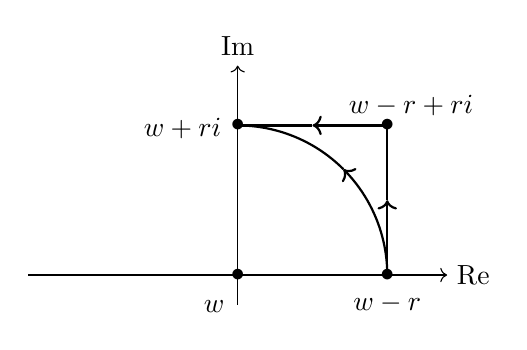
\begin{tikzpicture}[scale=1.9]
            % Axes
            \draw[->] (-1.4,0) -- (1.4,0) node[right] {$\Re$};
            \draw[->] (0,-0.2) -- (0,1.4) node[above] {$\Im$};
        
            % Quarter-circle contour
            \draw[thick, domain=0:45, ->] plot ({cos(\x)}, {sin(\x)});
            \draw[thick, domain=45:90, -] plot ({cos(\x)}, {sin(\x)});

            % Rectangular contour
            \draw[thick, ->] (1,0) -- (1,0.5);
            \draw[thick, -] (1,0.5) -- (1,1);
            \draw[thick, ->] (1,1) -- (0.5,1);
            \draw[thick, -] (0.5,1) -- (0,1);

            % Points of interest
            \labelledpoint{0}{0}{-0.3}{-0.8}{$w$}
            \labelledpoint{1}{0}{0}{-0.8}{$w - r$}
            \labelledpoint{1}{1}{0.3}{-0.2}{$w - r + ri$}
            \labelledpoint{0}{1}{-0.7}{-0.5}{$w + ri$}
        \end{tikzpicture}
        \caption{Contours for which \Cref{Ch4:Thm:CGTRectCircle} holds.}
    \end{subfigure} 
    \hfill
    \begin{subfigure}{0.48\linewidth}
        \centering
        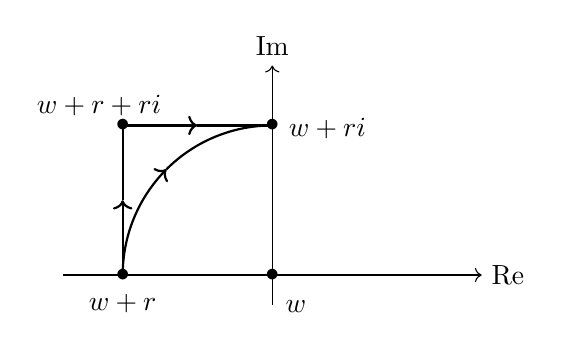
\begin{tikzpicture}[scale=1.9]
            % Axes
            \draw[->] (-1.4,0) -- (1.4,0) node[right] {$\Re$};
            \draw[->] (0,-0.2) -- (0,1.4) node[above] {$\Im$};
        
            % Quarter-circle contour
            \draw[thick, domain=180:135, ->] plot ({cos(\x)}, {sin(\x)});
            \draw[thick, domain=135:90, -] plot ({cos(\x)}, {sin(\x)});

            % Rectangular contour
            \draw[thick, ->] (-1,0) -- (-1,0.5);
            \draw[thick, -] (-1,0.5) -- (-1,1);
            \draw[thick, ->] (-1,1) -- (-0.5,1);
            \draw[thick, -] (-0.5,1) -- (0,1);

            % Points of interest
            \labelledpoint{0}{0}{0.3}{-0.8}{$w$}
            \labelledpoint{-1}{0}{0}{-0.8}{$w + r$}
            \labelledpoint{-1}{1}{-0.3}{-0.2}{$w + r + ri$}
            \labelledpoint{0}{1}{0.7}{-0.5}{$w + ri$}
        \end{tikzpicture}
        \caption{Contours for which an analogous result holds.}
        \label{Ch4:Subfig:CGTRectCircle_Alt}
    \end{subfigure} 
    \caption{The contour deformations permitted by \Cref{Ch4:Thm:CGTRectCircle}.}
\end{figure}

We now prove that $a$ is indeed a $+1$-eigenfunction of the Fourier transform.

\subsection{The $+1$-Eigenfunction}

The Fourier transform acts very interestingly on $a$. Recall from \Cref{Ch3:Thm:FourierSchwartz_CLE} that the Fourier transform is a linear isomorphism of Schwartz spaces. Since $I_1, \ldots, I_6$ are Schwartz, so are their compositions with the norm-squared function. Hence, for all $x \in \R^8$,
\begin{align*}
    \F\of{a(x)}
    % = \F\of{I_1\of{\norm{x}^2}} + \F\of{I_2\of{\norm{x}^2}} + \F\of{I_3\of{\norm{x}^2}} + \F\of{I_4\of{\norm{x}^2}} + \F\of{I_5\of{\norm{x}^2}} + \F\of{I_6\of{\norm{x}^2}}
    = \F\of{\sum_{j=1}^{6} I_j\of{\norm{x}^2}}
    = \sum_{j=1}^{6} \F\of{I_j\of{\norm{x}^2}}
\end{align*}

The strategy to show that $\F\of{a} = a$ will be to show that $\F$ acts on the $I_j\of{\norm{x}^2}$ in the following manner:\footnote{Note that we are abusing notation by denoting the function $x \mapsto I_j\of{\norm{x}^2} \in \Sch\of{\R^8, \C}$ by $I_j\of{\norm{x}^2}$.}
\begin{align}
    \F\of{I_1\of{\norm{x}^2} + I_2\of{\norm{x}^2}} &= I_3\of{\norm{x}^2} + I_4\of{\norm{x}^2} \label{Ch4:Eq:a_is_eig_perm_12_34} \\
    \F\of{I_3\of{\norm{x}^2} + I_4\of{\norm{x}^2}} &= I_1\of{\norm{x}^2} + I_2\of{\norm{x}^2} \label{Ch4:Eq:a_is_eig_perm_34_12} \\
    \F\of{I_5\of{\norm{x}^2}} &= I_6\of{\norm{x}^2} \label{Ch4:Eq:a_is_eig_perm_5_6} \\
    \F\of{I_6\of{\norm{x}^2}} &= I_5\of{\norm{x}^2} \label{Ch4:Eq:a_is_eig_perm_6_5}
\end{align}
Since, in addition to being Schwartz, all the $I_j\of{\norm{x}^2}$ (and their sums) are radial, \Cref{Ch3:Prop:RadialSchwartzFourier} tells us that \eqref{Ch4:Eq:a_is_eig_perm_34_12} and \eqref{Ch4:Eq:a_is_eig_perm_6_5} follow from \eqref{Ch4:Eq:a_is_eig_perm_12_34} and \eqref{Ch4:Eq:a_is_eig_perm_5_6} respectively. We now prove \eqref{Ch4:Eq:a_is_eig_perm_12_34} and \eqref{Ch4:Eq:a_is_eig_perm_5_6}.

As a preliminary step, though, we need to show integrability.

\begin{boxproposition}\label{Ch4:Prop:FourierIntegralConvergence_Ij}
    Fix $1 \leq j \leq 6$, and write $I_j(r) = \int_{X_j} f(r, z) \, \diff{z}$. Then, the Fourier Integral
    \begin{align*}
        \F\of{I_j\of{\norm{x}^2}}\of{\xi} = \int_{\R^8} \int_{X_j} \abs{f\of{\norm{x}^2, z} \, e^{-2 \pi i \cycl{x, \xi}}} \, \diff{z} \, \diff{x}
    \end{align*}
    converges for all $\xi \in \R^8$.
\end{boxproposition}
\begin{proof}
    Fix $\xi \in \R^8$. Note that we can disregard the $e^{-2 \pi i \cycl{x, \xi}}$ factor since it has absolute value $1$: the only reason we mention it is to emphasise that we are proving that the Fourier integral converges absolutely. Effectively, we need to show that the function
    \begin{align*}
        (x, z) \mapsto f\of{\norm{x}^2, z}
    \end{align*}
    admits an absolutely convergent integral over $\R^8 \times X_j$ with respect to the product measure.
    
    It has been formally verified that \href{https://github.com/leanprover-community/mathlib4/blob/5a2eaa85c555c4263e15928cef249cbaad2eb2d2/Mathlib/MeasureTheory/Integral/Prod.lean#L222-L238}{proving this is equivalent to proving the following two facts}.

    \begin{enumerate}
        \item \textbf{The integral over $X_j$ of the function $z \mapsto f\of{\norm{x}^2, z}$ is absolutely convergent for almost every $x \in \R^8$.}
        
        This is actually true for all $x$, and follows from the arguments in \Cref{Ch4:Subec:Schwartzness_a}.
        
        \item \textbf{The integral over $\R^8$ of the function $x 
        \mapsto \int_{X_j} \abs{f\of{\norm{x^2}, z}} \diff{z}$ is absolutely convergent.}
        
        By inspection, the arguments in \Cref{Ch4:Subec:Schwartzness_a} bound the function $r \mapsto \int_{X_j} \abs{f\of{r, z}} \diff{z}$ by a Schwartz function. Composing with the norm squared preserves Schwartzness by \Cref{Ch3:Prop:Multidimensional_Schwartz_of_Schwartz}, so we can bound the function $x \mapsto \int_{X_j} \abs{f\of{\norm{x}^2, z}} \diff{z}$ by a Schwartz function. It has been formally verified that \href{https://github.com/leanprover-community/mathlib4/blob/5a2eaa85c555c4263e15928cef249cbaad2eb2d2/Mathlib/Analysis/Distribution/SchwartzSpace.lean#L1095-L1097}{Schwartz functions are integrable}, so the integral over $\R^8$ of the function $x \mapsto \int_{X_j} \abs{f\of{\norm{x}^2, z}} \diff{z}$ must be absolutely convergent.
    \end{enumerate}
We can therefore conclude that the Fourier integral converges absolutely.
\end{proof}

Note that the above proposition is stronger than showing merely that the $I_j\of{\norm{x}^2}$ are integrable, as that does not imply that the integrands of the $I_j\of{\norm{x}^2}$ are integrable with respect to the product measure on $\R^8 \times X_j$. \Cref{Ch4:Prop:FourierIntegralConvergence_Ij}, however, does imply this, and we will need this to swap integrals using Fubini's theorem to prove the eigenfunction property.

\begin{boxlemma}\label{Ch4:Lemma:Fourier_I_1_add_I_2_eq_I_3_add_I_4}
    The Fourier transform % $\F : \Sch\of{\R^8, \C} \to \Sch{\R^8, \C}$
    maps $I_1\of{\norm{x}^2} + I_2\of{\norm{x}^2}$ to $I_3\of{\norm{x}^2} + I_4\of{\norm{x}^2}$.
\end{boxlemma}
\begin{proof}
    Since $\F$ acts linearly, we can treat $I_1$ and $I_2$ separately. For the purpose of this proof, denote the Fourier transforms of $I_1\of{\norm{x}^2}$ and $I_2\of{\norm{x}^2}$ by $F_1$ and $F_2$ respectively. Fix $\xi \in \R^8$. The integrability condition in \Cref{Ch4:Prop:FourierIntegralConvergence_Ij} allows us to change the order of integration below:
    \begin{align*}
        F_1\of{\xi} &= \int_{\R^8} \parenth {\int_{-1}^{-1 + i} \phi_0\of{\frac{-1}{z+1}} \, \parenth{z + 1}^2 \, e^{\pi i \norm{x}^2 z} \, \diff{z}} e^{-2\pi i \cycl{x, \xi}} \, \diff{x} \\
        &= \int_{-1}^{-1 + i} \phi_0\of{\frac{-1}{z+1}} \, \parenth{z + 1}^2 \parenth{\int_{\R^8} e^{\pi i \norm{x}^2 z} e^{-2\pi i \cycl{x, \xi} \diff{x}}} \, \diff{z}
    \end{align*}
    We can express $F_2$ in an analogous fashion. In both cases, the inner integral is exactly the Fourier integral of a Gaussian: in the notation of \Cref{Ch4:Thm:GaussianFourier}, $b = \pi i z$, and since $\Im(z) = \Re\of{i z} > 0$, we may apply the theorem to conclude that the inner integral is just
    \begin{align*}
        \frac{1}{z^4} \, e^{-\pi i \norm{\xi}^2 / z}
    \end{align*}
    We may therefore write
    \begin{align*}
        F_1\of{\xi} &= \int_{-1}^{-1 + i} \phi_0\of{\frac{-1}{z+1}} \, \parenth{z + 1}^2z^{-4} \, e^{\pi i \norm{\xi}^2 \parenth{\frac{-1}{z}}} \, \diff{z} \\
        F_2\of{\xi} &= \int_{-1 + i}^{i} \phi_0\of{\frac{-1}{z+1}} \, \parenth{z + 1}^2z^{-4} \, e^{\pi i \norm{\xi}^2 \parenth{\frac{-1}{z}}} \, \diff{z}
    \end{align*}
    We make a change of variables $w = \frac{-1}{z}$ in the above integrals. This Möbius transformation turns the vertical and horizontal contours in $F_1$ and $F_2$ into quarter-circular contours that we denote $\gamma_1$ and $\gamma_2$ respectively. See \Cref{Ch4:Fig:Eigenfunction_Mobius_Contours}.

    \begin{figure}[htb]
        \centering
        \begin{subfigure}{0.4\linewidth}
            \centering
            \begin{tikzpicture}[scale=1.9]
                % Axes
                \draw[->] (-1.4,0) -- (1.4,0) node[right] {$\Re$};
                \draw[->] (0,-0.2) -- (0,1.4) node[above] {$\Im$};
    
                % F_1
                \draw[thick, ->] (-1,0) -- (-1,0.5);
                \draw[thick, -] (-1,0.5) -- (-1,1);

                % F_2
                \draw[thick, ->] (-1,1) -- (-0.5,1);
                \draw[thick, -] (-0.5,1) -- (0,1);
    
                % Points of interest
                % \labelledpoint{0}{0}{0.3}{-0.8}{$0$}
                \labelledpoint{-1}{0}{0}{-0.8}{$-1$}
                \labelledpoint{-1}{1}{-0.3}{-0.2}{$-1 + i$}
                \labelledpoint{0}{1}{0.3}{-0.4}{$i$}
            \end{tikzpicture}
            \caption{Before the transformation}
        \end{subfigure}
        \begin{subfigure}{0.1\linewidth}
            \vfill
            \[ \leadsto \]
            \vspace{5em}
        \end{subfigure}
        \begin{subfigure}{0.4\linewidth}
            \centering
            \begin{tikzpicture}[scale=1.9]
                % Axes
                \draw[->] (-1.4,0) -- (1.4,0) node[right] {$\Re$};
                \draw[->] (0,-0.2) -- (0,1.4) node[above] {$\Im$};
            
                % \gamma_1
                \draw[thick, domain=0:45, ->] plot ({0.5 + 0.5 * cos(\x)}, {0.5 * sin(\x)}) node[below left] {$\gamma_1$};
                \draw[thick, domain=45:90, -] plot ({0.5 + 0.5 * cos(\x)}, {0.5 * sin(\x)});

                % \gamma_2
                \draw[thick, domain=0:45, ->] plot ({0.5 * cos(\x)}, {0.5 + 0.5 * sin(\x)}) node[below left] {$\gamma_2$};
                \draw[thick, domain=45:90, -] plot ({0.5 * cos(\x)}, {0.5 + 0.5 * sin(\x)});
    
                % Points of interest
                % \labelledpoint{0}{0}{0.3}{-0.8}{$w$}
                \labelledpoint{1}{0}{0}{-0.8}{$1$}
                \labelledpoint{0.5}{0.5}{0.6}{-0.2}{$\frac{1}{2} + \frac{1}{2}i$}
                \labelledpoint{0}{1}{-0.3}{-0.4}{$i$}
            \end{tikzpicture}
            \caption{After the transformation}
        \end{subfigure}
        \caption{The effect of the Möbius transformation $z \mapsto -1/z$ on the contours of $F_1$ and $F_2$}
        \label{Ch4:Fig:Eigenfunction_Mobius_Contours}
    \end{figure}
    Treating $\xi$ as a constant and denoting
    \begin{align*}
        f(w) := \phi_0\of{-1 - \frac{1}{w - 1}} \, \parenth{\frac{-1}{w} + 1}^2 w^2 \, e^{\pi i \norm{\xi}^2 w}
    \end{align*}
    we can distribute the $w^2$ term and use the fact that $\phi_0$ is $1$-periodic (cf. \eqref{Ch4:Eq:phi_0_add_one}) to write
    \begin{align*}
        f(w) = \phi_0\of{\frac{-1}{w - 1}} \, \parenth{w - 1}^2 \, e^{\pi i \norm{\xi}^2 w}
    \end{align*}
    we note that $f$ is holomorphic (in $w$) on the upper half-plane. \Cref{Ch4:Thm:CGTRectCircle} then tells us the following.
    \begin{align*}
        F_1\of{\xi}
        &= \int_{\gamma_1} f(w) \, \diff{w}
        = \int_{1}^{1 + \frac{1}{2}i} f(w) \, \diff{w}
        + \int_{1 + \frac{i}{2}i}^{\frac{1}{2} + \frac{1}{2}i} f(w) \, \diff{w} \\
        F_2\of{\xi}
        &= \int_{\gamma_2} f(w) \, \diff{w}
        = \int_{\frac{1}{2} + \frac{1}{2}i}^{\frac{1}{2} + i} f(w) \, \diff{w}
        + \int_{\frac{1}{2} + i}^{i} f(w) \, \diff{w}
    \end{align*}
    The \CGT\ for rectangles, which has been \href{https://github.com/leanprover-community/mathlib4/blob/88928cefd7edb1ba61623bffd4e86389dfe1f648/Mathlib/Analysis/Complex/CauchyIntegral.lean#L245}{formally verified}, tells us that
    \begin{align*}
        \int_{1 + \frac{i}{2}i}^{\frac{1}{2} + \frac{1}{2}i} f(w) \, \diff{w}
        + \int_{\frac{1}{2} + \frac{1}{2}i}^{\frac{1}{2} + i} f(w) \, \diff{w}
        = \int_{1 + \frac{1}{2}i}^{1+i} f(w) \, \diff{w}
        + \int_{1+i}^{\frac{1}{2} + i} f(w) \, \diff{w}
    \end{align*}
    Therefore, we can express $F_1 + F_2$ in the following manner:
    \begin{align*}
        F_1\of{\xi} + F_2\of{\xi}
        &= \int_{1}^{1 + \frac{1}{2}i} f(w) \, \diff{w}
        + \parenth{\int_{1 + \frac{i}{2}i}^{\frac{1}{2} + \frac{1}{2}i} f(w) \, \diff{w}
        + \int_{\frac{1}{2} + \frac{1}{2}i}^{\frac{1}{2} + i} f(w) \, \diff{w}}
        + \int_{\frac{1}{2} + i}^{i} f(w) \, \diff{w} \\
        &= \parenth{\int_{1}^{1 + \frac{1}{2}i} f(w) \, \diff{w}
        + \int_{1 + \frac{1}{2}i}^{1+i} f(w) \, \diff{w}}
        + \parenth{\int_{1+i}^{\frac{1}{2} + i} f(w) \, \diff{w}
        + \int_{\frac{1}{2} + i}^{i} f(w) \, \diff{w}} \\
        &= I_3\of{\norm{\xi}^2} + I_4\of{\norm{\xi}^2}
    \end{align*}
    as required. \Cref{Ch4:Fig:Eigenfunction_CauchyGoursat_a} shows how contours were modified over the course of this argument.
    \begin{figure}[hbt]
        \centering
        \begin{subfigure}{0.4\linewidth}
            \centering
            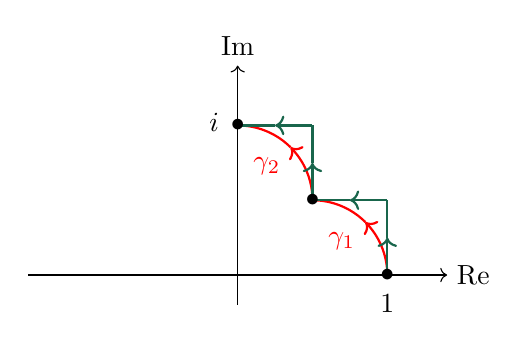
\begin{tikzpicture}[scale=1.9]
                % Axes
                \draw[->] (-1.4,0) -- (1.4,0) node[right] {$\Re$};
                \draw[->] (0,-0.2) -- (0,1.4) node[above] {$\Im$};
            
                % \gamma_1
                \draw[thick, domain=0:45, ->, red] plot ({0.5 + 0.5 * cos(\x)}, {0.5 * sin(\x)}) node[below left] {$\gamma_1$};
                \draw[thick, domain=45:90, -, red] plot ({0.5 + 0.5 * cos(\x)}, {0.5 * sin(\x)});

                % \gamma_2
                \draw[thick, domain=0:45, ->, red] plot ({0.5 * cos(\x)}, {0.5 + 0.5 * sin(\x)}) node[below left] {$\gamma_2$};
                \draw[thick, domain=45:90, -, red] plot ({0.5 * cos(\x)}, {0.5 + 0.5 * sin(\x)});

                % Rectangle 1
                \draw[thick, ->, darkgreen] (1, 0) -- (1, 0.25);
                \draw[thick, -, darkgreen] (1, 0.25) -- (1, 0.5);
                \draw[thick, ->, darkgreen] (1, 0.5) -- (0.75, 0.5);
                \draw[thick, -, darkgreen] (0.75, 0.5) -- (0.5, 0.5);

                % Rectangle 2
                \draw[thick, ->, darkgreen] (0.5, 0.5) -- (0.5, 0.75);
                \draw[thick, -, darkgreen] (0.5, 0.75) -- (0.5, 1);
                \draw[thick, ->, darkgreen] (0.5, 1) -- (0.25, 1);
                \draw[thick, -, darkgreen] (0.25, 1) -- (0, 1);
    
                % Points of interest
                % \labelledpoint{0}{0}{0.3}{-0.8}{$w$}
                \labelledpoint{1}{0}{0}{-0.8}{$1$}
                \labelledpoint{0.5}{0.5}{0.6}{-0.2}{}
                \labelledpoint{0}{1}{-0.3}{-0.4}{$i$}
            \end{tikzpicture}
            \caption{Changing contours from circles to rectangles}
        \end{subfigure}
        \hfill
        \begin{subfigure}{0.4\linewidth}
            \centering
            \begin{tikzpicture}[scale=1.9]
                % Axes
                \draw[->] (-1.4,0) -- (1.4,0) node[right] {$\Re$};
                \draw[->] (0,-0.2) -- (0,1.4) node[above] {$\Im$};
            
                % Rectangle 1
                \draw[thick, ->] (1, 0) -- (1, 0.25);
                \draw[thick, -] (1, 0.25) -- (1, 0.5);
                \draw[thick, ->, red] (1, 0.5) -- (0.75, 0.5);
                \draw[thick, -, red] (0.75, 0.5) -- (0.5, 0.5);

                % Rectangle 2
                \draw[thick, ->, red] (0.5, 0.5) -- (0.5, 0.75);
                \draw[thick, -, red] (0.5, 0.75) -- (0.5, 1);
                \draw[thick, ->] (0.5, 1) -- (0.25, 1);
                \draw[thick, -] (0.25, 1) -- (0, 1);

                % Rectangle Cauchy-Goursat
                \draw[thick, ->, darkgreen] (1, 0.5) -- (1, 0.75);
                \draw[thick, -, darkgreen] (1, 0.5) -- (1, 1);
                \draw[thick, ->, darkgreen] (1, 1) -- (0.75, 1);
                \draw[thick, -, darkgreen] (0.75, 1) -- (0.5, 1);
    
                % Points of interest
                % \labelledpoint{0}{0}{0.3}{-0.8}{$w$}
                \labelledpoint{1}{0}{0}{-0.8}{$1$}
                \labelledpoint{0.5}{0.5}{0.6}{-0.2}{}
                \labelledpoint{0}{1}{-0.3}{-0.4}{$i$}
            \end{tikzpicture}
            \caption{Changing rectangular contours to get $I_3$ and $I_4$}
        \end{subfigure}
        \caption{Applying the two versions of the \CGT\ to prove the result. In the proof, contours were changed from red to green.}
        \label{Ch4:Fig:Eigenfunction_CauchyGoursat_a}
    \end{figure}
\end{proof}

The proof that the Fourier transform maps $I_5$ to $I_6$ is nearly identical in structure but significantly simpler, because the Möbius transformation $z \mapsto \frac{-1}{z}$ simply maps the contour in $I_5$ to that in $I_6$ (and vice-versa). We omit the proof.

In summary, we have shown that the Fourier transform permutes the integrals that make up $a$, thereby not changing $a$. $a$ is thus an eigenfunction of $\F$ with eigenvalue $1$.

It is worth noting that the Möbius transformation $z \mapsto \frac{-1}{z}$ in the proof of \Cref{Ch4:Lemma:Fourier_I_1_add_I_2_eq_I_3_add_I_4} has derivative $\frac{1}{z^2}$, which reduces the $z^4$ term in the integrand to $z^2$, which matches the pattern in $I_3$ and $I_4$. However, the reason the $z^4$ term arises is that we take the $8$-dimensional Fourier transform of an $8$-dimensional Gaussian. This illustrates why it was necessary to treat $a$ as an $\R^8 \to \C$ function to show the eigenfunction property. More generally, despite Fourier transforms being linear isomorphisms of Schwartz spaces, the fact remains that in different Schwartz spaces, the Fourier transform operators may be fundamentally different, and linear maps between Schwartz spaces are not guaranteed to preserve the Fourier transform operator.

We now use similar techniques to show that $b$ is a Fourier eigenfunction with eigenvalue $-1$. % Just as we did with the proof of Schwartzness, we omit repetitive arguments and focus on the key distinctions between the two cases.

\subsection{The $-1$-Eigenfunction}
\section{Establishing the Double Zeroes Property}

% At some point earlier on, maybe in Chapter 3, we need to stress that double zeroes means double zeroes in the radial sense, except double zeroes after composition with just the norm and not the norm squared. (We are using norm squared so that we can prove Schwartzness. Just the norm isn't enough because the norm isn't smooth.)

The way we prove that $a$ and $b$ have double zeroes at $E_8$ lattice points with norm $> \sqrt{2}$ (or at normalised $E_8$ lattice points with norm $> 1$) is by showing that $a\rad$ and $b\rad$ agree, for $r > 2$, with functions that have double zeroes at \textit{all} even integers. It will then follow that $a$ and $b$ have double zeroes at all points on the $E_8$ lattice with norm $> \sqrt{2}$, since all elements of $\Lambda_8$ have norm of the form $\sqrt{2n}$ for some $n \in \N$ (cf. \sorry).\todo{ADD RESULT TO E8 SECTION}

The strategy to prove these two equalities will be to perform a change of contours using a version of the Cauchy-Goursat Theorem and use the relations and transformation rules between the $\phi$- and $\psi$-functions to combine integrals so that the result is exactly $a\rad$ or $b\rad$.

The version of the Cauchy-Goursat Theorem we use is the following.

\begin{boxtheorem}[Cauchy-Goursat for Unbounded Contours]\label{Ch4:Thm:CauchyGoursat_Unbounded}
    Suppose $f : \C \to \C$ is a function such that $f(z) \to 0$ as $\Im(z) \to \infty$. Then, for all $x_1, y_1, x_2, y_2 \in \R$, if $f$ is holomorphic at $z$ for all $z \in \C$ with $x_1 < \Re(z) < x_2$ and $y_2 < \Im(z)$, then
    \begin{align*}
        \int_{x_1 + iy_1}^{x_1 + i\infty} f(z) \, \diff{z}
        = \int_{x_1 + iy_1}^{x_1 + iy_2} f(z) \, \diff{z}
        + \int_{x_1 + iy_2}^{x_2 + iy_2} f(z) \, \diff{z}
        + \int_{x_2 + iy_2}^{x_2 + i\infty} f(z) \, \diff{z}
    \end{align*}
    provided that $f$ is integrable on the unbounded vertical contours.
\end{boxtheorem}

\begin{wrapfigure}[7]{r}{0.4\linewidth}
    \vspace{-0.7em}
    \centering
    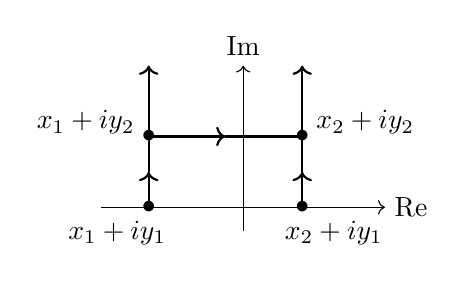
\begin{tikzpicture}[scale=1.5]
        % Axes
        \draw[->] (-1.2,0) -- (1.2,0) node[right] {$\Re$};
        \draw[->] (0,-0.2) -- (0,1.2) node[above] {$\Im$};
    
        % Contours
        \draw[thick, ->] (-0.8, 0) -- (-0.8,0.3);
        \draw[thick, ->] (-0.8,0.3) -- (-0.8, 1.2);
        \draw[thick, ->] (0.5, 0) -- (0.5,0.3);
        \draw[thick, ->] (0.5,0.3) -- (0.5, 1.2);
        \draw[thick, ->] (-0.8, 0.6) -- (-0.15, 0.6);
        \draw[thick] (-0.15, 0.6) -- (0.5, 0.6);
    
        % Points of interest
        \labelledpoint{-0.8}{0}{-0.4}{-0.8}{$x_1 + iy_1$}
        \labelledpoint{0.5}{0}{0.4}{-0.8}{$x_2 + iy_1$}
        \labelledpoint{-0.8}{0.6}{-0.8}{-0.3}{$x_1 + iy_2$}
        \labelledpoint{0.5}{0.6}{0.8}{-0.3}{$x_2 + iy_2$}
    \end{tikzpicture}
    \caption{Visualising the contours in \Cref{Ch4:Thm:CauchyGoursat_Unbounded}.}  
\end{wrapfigure}

We discuss the informal and formal proofs of this theorem in \Cref{Ch5:Sec:Cauchy-Goursat}.

For both $a\rad$ and $b\rad$, we begin by their alternate expressions for them. We then make estimates to prove that the integrals in these expressions converge. We finally manipulate the expressions and apply \Cref{Ch4:Thm:CauchyGoursat_Unbounded} to show that they do, indeed, agree with $a\rad$ and $b\rad$ on inputs $> 2$.

\subsection{The $+1$-Eigenfunction}

We begin by defining the integral by which we represent $a\rad$.

\begin{boxdefinition}[Alternate Representation of $a$]
    Define $d : \parenth{2, \infty} \to \C$ by
    \begin{align*}
        d\of{r} = -4 \sinsq{\frac{\pi r}{2}} \int_{0}^{i\infty} \phi_0\of{\frac{-1}{z}} \, z^2 \, e^{\pi i r z} \, \diff{z}
    \end{align*}
    for all $r \in \parenth{2, \infty}$.
\end{boxdefinition}

It is clear that we can parametrise the integral in $d$ by $z = it$ for $t \in \parenth{0, \infty}$, and write
\begin{align}
    d(r) = 4i \sinsq{\frac{\pi r}{2}} \int_{0}^{\infty} \phi_0\of{\frac{i}{t}} \, t^2 \, e^{-\pi r t} \, \diff{t}
    \label{Ch4:Eq:d_parametrised}
\end{align}

We begin by showing that this integral converges for $r > 2$. We do this by estimating the integrand.

\begin{boxlemma}
    $\exists C_0 > 0$ such that for $t \in \parenth{0, 2}$, $\abs{\phi_0\of{\frac{i}{t}}} \leq C_0 \, e^{-2\pi/t}$.
\end{boxlemma}
\begin{proof}
    The result then follows immediately from \eqref{Ch4:Eq:PolyFourierCoeffBound_phi_0}, with $z = i/t$.
\end{proof}

We can hence conclude that for $t \in \parenth{0, 2}$, the integrand in \eqref{Ch4:Eq:d_parametrised} is bounded:
\begin{align*}
    \abs{\phi_0\of{\frac{i}{t}} \, t^2 \, e^{-\pi r t}} 
    \leq 4 C_0 \, e^{-2\pi / t} \, e^{-\pi r t}
    \leq 4 C_0
\end{align*}

We can also estimate the integrand for $t \geq 2$.

\begin{boxlemma}\label{Ch4:Lemma:d_integral_estimate_above}
    $\exists C > 0$ such that for $t \geq 2$, $\abs{\phi_{0}\of{\frac{i}{t}}} \leq C t^{-2} e^{2\pi t}$.
\end{boxlemma}
\begin{proof}
    From \eqref{Ch4:Eq:phi_0_neg_inv}, we know that for all $t \geq 2$,
    \begin{align*}
        \abs{\phi_0\of{\frac{i}{t}}}
        = \abs{\phi_{0}\of{\frac{-1}{it}}}
        \leq \abs{\phi_{0\of{it}}} + \frac{12}{\pi t} \abs{\phi_{-2}\of{it}} + \frac{36}{\pi^2 t^2} \abs{\phi_{-4}\of{it}}
    \end{align*}
    Estimating each of these terms using \Cref{Ch4:Lemma:PolyFourierCoeffBound_Apply_a}, we know $\exists C_0, C_{-2}, C_{-4} > 0$ such that
    \begin{align*}
        \abs{\phi_{0}\of{it}} + \frac{12}{\pi t} \abs{\phi_{-2}\of{it}} + \frac{36}{\pi^2 t^2} \abs{\phi_{-4}\of{it}}
        \leq C_0 e^{-2 \pi t} + \frac{12}{\pi t} C_{-2} + \frac{36}{\pi^2 t^2} C_{-4} e^{2 \pi t}
    \end{align*}
    For $t \geq 2$, $C_0 e^{-2 \pi t}$ and $\frac{12}{\pi t} C_{-2}$ are clearly bounded by constants, and the growth of the above expression is dominated by $t^{-2} e^{2\pi t}$. Hence, we can conclude that $\exists C > 0$ such that for $t \geq 2$, $\abs{\phi_0\of{\frac{i}{t}}} \leq C t^{-2} e^{2 \pi t}$, as required.
\end{proof}

We can hence conclude that for $t \geq 2$, the integrand in \eqref{Ch4:Eq:d_parametrised} is bounded by an integrable function:
\begin{align*}
    \abs{\phi_0\of{\frac{i}{t}} \, t^2 \, e^{-\pi r t}} 
    \leq C \parenth{t^{-2} e^{2\pi t}} \parenth{t^2 e^{-\pi r t}}
    = C e^{\pi t \parenth{2 - r}}
\end{align*}
Here, we require $r > 2$ so that the exponent is negative. Since $d$ was defined precisely on such $r$, we can conclude that the integral in the definition of $d$ converges absolutely.

Arguing as above yields another important result.
\begin{boxlemma}
    For all $r > 2$ and $z \in \Halfplane$, as $\Im(z) \to \infty$,
    \begin{align*}
        \phi_{0}\of{\frac{-1}{z}} \, z^2 \, e^{\pi i r z} \to 0
    \end{align*}
\end{boxlemma}
\begin{proof}[Proof sketch]
    We do not offer more than a sketch here because the proof is almost identical to that of \Cref{Ch4:Lemma:d_integral_estimate_above}. The idea is to apply \eqref{Ch4:Eq:phi_0_neg_inv}, multiply through, apply \Cref{Ch4:Lemma:PolyFourierCoeffBound_Apply_a} to bound the expression in absolute value, and use the fact that $r > 2$ to conclude that the bound decays exponentially as $\Im(z) \to \infty$.
\end{proof}

The function $z \mapsto \phi_{0}\of{\frac{-1}{z}} \, z^2 \, e^{\pi i r z}$ is also holomorphic on $\Halfplane$, a fact that is again seen by applying \eqref{Ch4:Eq:phi_0_neg_inv} and the fact that the numerators of the $\phi$-function are holomorphic and the denominators are non-vanishing on $\Halfplane$.

We are now ready to show the following.

\begin{boxproposition}
    For all $r > 2$, $d(r) = a\rad(r)$.
\end{boxproposition}
\begin{proof}
    Fix $r > 2$. We begin by performing the following manipulation:
    \begin{align*}
        -4 \sinsq{\frac{\pi r}{2}}
        = -4 \parenth{\frac{e^{i \pi r / 2} - e^{-i \pi r / 2}}{2i}}^2
        = \parenth{e^{i \pi r / 2} - e^{- i \pi r / 2}}^2
        = e^{i \pi r} - 2 + e^{-i \pi r}
    \end{align*}
    Therefore, for all $r > 2$,
    \begin{align*}
        d(r)
        &= -4 \sinsq{\frac{\pi r}{2}} \int_{0}^{i \infty} \phi_0\of{\frac{-1}{z}} \, z^2 \, e^{\pi i r z} \, \diff{z}
        = \parenth{e^{i \pi r} - 2 + e^{-i \pi r}} \int_{0}^{i \infty} \phi_0\of{\frac{-1}{z}} \, z^2 \, e^{\pi i r z} \, \diff{z} \\
        &= \int_{0}^{i \infty} \phi_0\of{\frac{-1}{z}} z^2 \, e^{\pi i r \parenth{z + 1}} \, \diff{z}
        -2 \int_{0}^{i \infty} \phi_0\of{\frac{-1}{z}} z^2 \, e^{\pi i r z} \, \diff{z}
        + \int_{0}^{i \infty} \phi_0\of{\frac{-1}{z}} z^2 \, e^{\pi i r \parenth{z - 1}} \, \diff{z}
    \end{align*}
    By a simple change of variables, we can rewrite the first and third integrals as follows. We can also split the second integral into two parts as shown below.
    \begin{align*}
        \int_{0}^{i \infty} \phi_0\of{\frac{-1}{z}} z^2 \, e^{\pi i r \parenth{z - 1}} \, \diff{z}
        &=
        \int_{-1}^{-1 + i \infty} \phi_0\of{\frac{-1}{z + 1}} \parenth{z + 1}^2 \, e^{\pi i r z} \, \diff{z} \\
        \int_{0}^{i \infty} \phi_0\of{\frac{-1}{z}} z^2 \, e^{\pi i r \parenth{z + 1}} \, \diff{z}
        &=
        \int_{1}^{1 + i \infty} \phi_0\of{\frac{-1}{z - 1}} \parenth{z - 1}^2 \, e^{\pi i r z} \, \diff{z} \\
        -2 \int_{0}^{i \infty} \phi_0\of{\frac{-1}{z}} z^2 \, e^{\pi i r z} \, \diff{z}
        &=
        -2 \int_{0}^{i} \phi_0\of{\frac{-1}{z}} z^2 \, e^{\pi i r z} \, \diff{z}
        -2 \int_{i}^{i \infty} \phi_0\of{\frac{-1}{z}} z^2 \, e^{\pi i r z} \, \diff{z} \\
        &= I_5(r) - 2\int_{i}^{i \infty} \phi_0\of{\frac{-1}{z}} z^2 \, e^{\pi i r z} \, \diff{z}
    \end{align*}
    We can now apply \Cref{Ch4:Thm:CauchyGoursat_Unbounded} to the first and third integrals, noting that the required integrability conditions do hold because the integrals making up $d$ and $a\rad$ converge absolutely.
    \begin{align*}
        \int_{-1}^{-1 + i \infty} \phi_0\of{\frac{-1}{z + 1}} \parenth{z + 1}^2 \, e^{\pi i r z} \, \diff{z}
        =& \int_{-1}^{-1 + i} \phi_0\of{\frac{-1}{z + 1}} \parenth{z + 1}^2 \, e^{\pi i r z} \, \diff{z} \\
        &+ \int_{-1 + i}^{i} \phi_0\of{\frac{-1}{z + 1}} \parenth{z + 1}^2 \, e^{\pi i r z} \, \diff{z} \\
        &+ \int_{i}^{i \infty} \phi_0\of{\frac{-1}{z + 1}} \parenth{z + 1}^2 \, e^{\pi i r z} \, \diff{z} \\
        =& I_1(r) + I_2(r) + \int_{i}^{i \infty} \phi_0\of{\frac{-1}{z + 1}} \parenth{z + 1}^2 \, e^{\pi i r z} \, \diff{z} \\
        \int_{1}^{1 + i \infty} \phi_0\of{\frac{-1}{z - 1}} \parenth{z - 1}^2 \, e^{\pi i r z} \, \diff{z}
        =& \int_{1}^{1 + i} \phi_0\of{\frac{-1}{z - 1}} \parenth{z - 1}^2 \, e^{\pi i r z} \, \diff{z} \\
        &+ \int_{1 + i}^{i} \phi_0\of{\frac{-1}{z - 1}} \parenth{z - 1}^2 \, e^{\pi i r z} \, \diff{z} \\
        &+ \int_{i}^{i \infty} \phi_0\of{\frac{-1}{z - 1}} \parenth{z - 1}^2 \, e^{\pi i r z} \, \diff{z} \\
        =& I_3(r) + I_4(r) + \int_{i}^{i \infty} \phi_0\of{\frac{-1}{z - 1}} \parenth{z - 1}^2 \, e^{\pi i r z} \, \diff{z}
    \end{align*}
    Hence, we can express $d(r)$ as the sum of the following six integrals:
    \begin{align*}
        d(r) =& I_1(r) + I_2(r) + I_3(r) + I_4(r) + I_5(r) \\
        &+ \int_{i}^{i\infty} \parenth{
            \phi_0\of{\frac{-1}{z + 1}} \parenth{z + 1}^2 \, e^{\pi i r z} +
            \phi_0\of{\frac{-1}{z - 1}} \parenth{z - 1}^2 \, e^{\pi i r z} - 2
            \phi_0\of{\frac{-1}{z}} z^2 \, e^{\pi i r z}
        } \, \diff{z}
    \end{align*}
    One can show, by applying \eqref{Ch4:Eq:phi_0_neg_inv} and simplifying, that
    \begin{align*}
        \phi_0\of{\frac{-1}{z + 1}} \parenth{z + 1}^2 +
        \phi_0\of{\frac{-1}{z - 1}} \parenth{z - 1}^2 +
        \phi_0\of{\frac{-1}{z}} z^2 = 2\phi_0
    \end{align*}
    Hence, the sixth integral above is precisely $I_6$, proving that $d(r) = a\rad(r)$ for all $r > 2$.
\end{proof}

The factor of $-4\sinsq{\pi r / 2}$ in the definition of $d$ then ensures that $a\rad$ has double zeroes at all even integers except possibly $0$ and $\pm 2$, which allows us to conclude that $a$ has double zeroes at all points in $\R^8$---particularly those lying on $\Lambda_8$---with norm of the form $\sqrt{2n}$ for $n \in \N \setminus \set{0, 1}$.

\subsection{The $-1$-Eigenfunction}
\section{The Magic of $g$}
\label{Ch4:Sec:g_Properties}

% Not yet sure how this section should look
\chapter{Viazovska's Magic Function, Formally}
\thispagestyle{empty}
% I really don't like this chapter name because idt it reflects the essence of the chapter, which is "the key aspects of the formalisation/challenges faced and overcome". But that's not a good title either. Gotta find something in the middle!

\section{The Formalisation Effort: A Broad Overview}
\label{Ch5:Sec:Gen_Overview_of_Formalisation}

As was mentioned in \Cref{Ch1:Chapter}, the formalisation of Viazovska's proof was initiated by Viazovska and Hariharan in March 2024. A public announcement was made in June 2024, following which Birkbeck, Lee, and Ma joined the collaboration. Macbeth and Mehta too have made significant contributions since October 2024.

All code pertaining to the formalisation of the contents of \Cref{Ch4:Chapter} that does not come from the broader theory of modular forms has been written solely by the author, with advice from Mehta. While the formalisation is not complete, the author's progress is best interpreted as providing important tools and frameworks that will significantly ease the remainder of the formalisation.

The most significant difference between the author's exposition and Viazovska's original proof is that the author uses six defining integrals instead of four, with all contours being rectangular. The reason this is useful is that a formal version of the \CGT\ that exists in \mathlib\ for rectangular contours. A crucial step in \Cref{Ch4:Sec:Double_Zeroes} involves deforming unbounded contours, and the author formalised an appropriate version of the \CGT\ to work around this problem. The author's work builds on the \mathlib\ version for bounded rectangular contours, and hypothesised that it would be easier to adapt the definitions and proofs preceding that of double zeroes to a function defined using rectangular contours than it would to prove an unbounded version of the \CGT\ involving circular or triangular contours. Unfortunately, the proof of the eigenfunction property is not compatible with rectangular contours, but the author remains confident in the possibility of a workaround. We continue this discussion in \Cref{Ch5:Sec:Cauchy-Goursat}.

Viazovska's proof is heavy on computation. At the beginning of this M4R, the author was unaccustomed to proving computationally intensive results in Lean. While early attempts involved writing lengthy calculation lemmas, the author soon discovered that breaking computations into several lemmas corresponding to individual steps improved not only readability but also compilation time. The author's formal proof of \Cref{SP:PolyFourierCoeffBound}, for example, consists of thirteen auxiliary lemmas corresponding to individual steps, and the author's formal proofs of the bounds on each of the $I_1, \ldots, I_6$ are spread across two files: one with alternate expressions for all the $I_j$s and one with bounds on the $I_j$ in question. A further advantage of this approach is its isolation of dependencies that are difficult to formalise, such as convergence results for sums, products and integrals that arise in either the statement or proof of a result. In some cases, one finds workarounds: for instance, when bounding the $I_j$, the author realised that the proof that the $I_j$ converge absolutely is not necessary because of the way integrals are defined in \mathlib. The necessity of such excruciating detail in formal proofs was the author's key motivator to provide detailed arguments in \Cref{Ch4:Chapter}: the author's intent is for the proofs in this thesis to be a bridge between the informal and the formal, building on Viazovska's arguments in \cite[\S 7]{blueprint}.

For the remainder of this section, we briefly discuss two contributions the author made to the formalisation that account for differences, however minor, between Viazovska's original proof and the author's exposition. We then move onto two dedicated sections that respectively describe the metaprogramming approach implemented by Macbeth, Xie and the author and the challenges associated with the \CGT\ and how some, though not all, of them have been overcome.

\subsection{A Systematic Approach to Bounding Integrals}
\label{Ch5:Subsec:Bounding_Integrals}

Before the idea of rectangular contours, the author attempted to express $I_1 + I_2$ using a triangular contour. In fact, the author succeeded in bounding it by following the arguments in \cite{Viazovska8}. However, once the idea of rectangular contours was conceived, the author realised that six integrals would need to be bounded instead of four, as in \cite{Viazovska8}. The author hence decided to systematise his approach to maximise reusability of code. Indeed, that the proofs of \Cref{Ch4:Eq:Bound_I1_I3_I5,Ch4:Eq:Bound_I2_I4,Ch4:Eq:Bound_I6} are direct informalisations of the formal proofs found in the repository. There is one file per integral in the directory \lstinline|MagicFunction.a.IntegralEstimates|, but the structure is nearly identical for those integrals bounded using the same techniques, reflecting the systematic nature of the approach. All specific references in this subsection will involve the $I_j$, though we emphasise, as we did in \Cref{Ch4:Subec:Schwartzness_b}, that the $J_j$ are similar.\todo{Maybe rephrase if we don't finish bounding the Js in time}

The integrals are defined using parametrisations involving a real variable, so that API on \lstinline|intervalIntegral| could be used. To maximise compatibility, the most frequently used versions of the $\phi$-functions and the parametrisations are extensions of these functions to $\C$ and $\R$ respectively that are $0$ outside of where they are meant to be defined. This is in line with the \mathlib\ style of defining constructions like sums, integrals and products to take trivial values outside when these constructions are not well-defined in informal mathematics. We now give a step-by-step breakdown of how the author bounded integrals in Lean.

\begin{enumerate}
    \item \underline{Expressing the integrands in a convenient form.}

    Aside from enhancing readability and underscoring the resemblance of the formal integrals to the informal integrals, parametrisations are a way to control the variable of integration. However, they come with a layer of syntax that is unhelpful for bounding. Hence, we define lemmas ending in \lstinline|_eq| and \lstinline|_eq'| to overcome them.
    
    \lstinline|_eq| lemmas expand the parametrisations and perform basic simplifications, such as separating a term of the form $e^{\pi i r\parenth{1 + it}}$ into $e^{\pi i r} \cdot e^{-\pi r t}$. \lstinline|_eq'| lemmas take any scalars arising from this process (such as a factor of $i$ from a parametrisation $z = 1 + it$) outside of the integral, which makes them easier to deal with when bounding the integral. These lemmas are proved in \lstinline|MagicFunction.a.Basic| for all $I_j$, whereas the remaining steps are proved in individual files in \lstinline|MagicFunction.a.IntegralEstimates|.

    \item \underline{Changing variables (first, third and fifth integrals only).}

    Informally and formally, the key to bounding the first, third, and fifth integrals of both eigenfunctions is to perform a change of variables $s = \frac{1}{t}$. We do this by applying \href{https://github.com/leanprover-community/mathlib4/blob/5a2eaa85c555c4263e15928cef249cbaad2eb2d2/Mathlib/MeasureTheory/Function/Jacobian.lean#L1199}{a previously formalised \mathlib\ result} using functions \lstinline|f|, \lstinline|f'| and \lstinline|g|, defined at the top of each file, denoting the variable change, its derivative, and the desired form of the integrand \textbf{after} the change of variables. Just as in this thesis, the author applied the convention of using \lstinline|s| to denote the integration variable after the change and \lstinline|t| to denote it before. An intermediate lemma navigates syntactic challenges, reconciling the integral in \lstinline|t| whose integrand is a composition \lstinline|g| with \lstinline|f|.

    \item \underline{Bounding the integrand.}

    By inspection, one sees that in \Cref{Ch4:Eq:Bound_I1_I3_I5,Ch4:Eq:Bound_I2_I4,Ch4:Eq:Bound_I6}, the bounds on the integrals actually come from bounds on the integrands. This is done formally using two lemmas, the first performing elementary bounds and the second applying \Cref{SP:PolyFourierCoeffBound}. The application of \Cref{SP:PolyFourierCoeffBound} is less straightforward for $I_2$ and $I_4$ because the condition $\Im(z) > \frac{1}{2}$ is more difficult to show (as seen in the informal proof of \Cref{Ch4:Eq:Bound_I2_I4} as well), so there are added helper lemmas for this.

    \item \underline{Bounding the integral.}

    This involves applying the \href{https://github.com/leanprover-community/mathlib4/blob/5a2eaa85c555c4263e15928cef249cbaad2eb2d2/Mathlib/MeasureTheory/Integral/Bochner/Basic.lean#L927}{triangle inequality} and \href{https://github.com/leanprover-community/mathlib4/blob/5a2eaa85c555c4263e15928cef249cbaad2eb2d2/Mathlib/MeasureTheory/Integral/Bochner/Set.lean#L645}{monotonicity of the integral}, which were formalised in \mathlib\ well before this project. Applying the former is straightforward, but applying the latter is not, because it requires integrability assumptions on the functions in question. The reason for this is that if $f \leq g$ and $f$ is integrable but $g$ is not, then the integral of $g$, as defined in Lean, is $0$. Fortunately, for nonnegative $f$ and $g$ (such as the absolute values of our integrands and the functions that bound them), only needs $g$ to be integrable. Integrability proofs for some bounding functions are currently \sorry s.
\end{enumerate}

The systematic nature of this approach makes it easy to reuse: the only differences between the computations for similar integrals are in the \lstinline|g|s and the \lstinline|_eq| and \lstinline|_eq'| lemmas that are invoked at various points. Thus, the overall complexity of the task was reduced substantially.

\subsection{A Schwartzness Bridge Across Dimensions}
\label{Ch5:Subsec:Schwartz_Bridge}

% THIS IS ACTUAL NONSENSE. NEED TO FIX THE LEAN BRIDGE BECAUSE WHILE IT IS TRUE IT IS COMPLETELY UNHELPFUL FOR THIS SITUATION.

In \cite{Viazovska8}, the proof that $a$ and $b$ are Schwartz functions involves showing that they were radially Schwartz. That is, Viazovska shows that $a(r)$ and $b(r)$ are Schwartz in $r$, these functions translating to $a\rad\of{r^2}$ and $b\rad\of{r^2}$ in our notation. There is a highly nontrivial step missing: a bridge between one-dimensional smooth, decaying functions and $8$ (and higher)-dimensional Schwartz functions. In this project, such a bridge was built formally so as to allow free translation between the radial and $\R^8$ settings.

First, we note that it is quite simple to formally build a bridge between one- and higher-dimensional Schwartz functions due to an \href{https://github.com/leanprover-community/mathlib4/blame/5a2eaa85c555c4263e15928cef249cbaad2eb2d2/Mathlib/Analysis/Distribution/SchwartzSpace.lean#L857}{intermediate result of immense import} formalised originally in Lean 3 by Moritz Doll and subsequently ported to \mathlib4.

Having discussed these general contributions, we discuss two very specific and profound contributions made by the author to the formalisation effort. We begin by discussing the development of a Lean tactic by Macbeth, Xie and the author.
\section{A Metaprogramming Approach}

\begin{comment}
Begin by saying a few words about what metaprogramming is. Then go into subsections. Idea:
1. Establish difficulty of doing computations in \C. Give examples, yes, but also stress that existing automation was unable to unpack the structural nuances of the way \C is defined. Also maybe talk about the whole "is I a numeral" debate, but I think this might be a rabbit-hole...
2. Talk about the algorithm behind norm_numI. Talk about the original version we worked on with Heather and Edison at/after metaprogramming and at Xena.
3. Say something about what Heather's latest modifications look like. Maybe also talk about how the approach can be generalised to quaternion algebras or splitting fields (what's similar and what's different between norm_numI and these things), but don't talk about the maths of either of these. Stress that this is still under development, and that this opens the door to a world of metaprogramming possibilities.
\end{comment}

In this section, we discuss an unexpected biproduct of this project: the development of a normalisation-simplification automation for performing computations in the complex numbers.

Lean, like other interactive theorem provers, primarily interacts with its users through \textbf{tactics}. Fundamentally, the proof of a theorem in Lean is given by a \textbf{proof term}, which can be thought of as a concise expression that captures the information of how the hypotheses or inputs of the theorem are transformed into its conclusion by giving exactly the conclusion into which these inputs are transformed. A tactic is a command that, when invoked by a Lean user, performs a step in the construction of the proof term for a theorem.

The most basic tactics can be thought of as being `syntax sugar' rather than invocations of computation or reasoning algorithms. Consider the following code.
\begin{lstlisting}[caption=A tactic-mode proof of the associativity of $\land$, label=Ch5:Listing:And_assoc_tactic]
example (P Q R : Prop) : P ∧ (Q ∧ R) ↔ (P ∧ Q) ∧ R := by
  constructor
  · intro h
    constructor
    · constructor
      · exact h.1
      · exact h.2.1
    · exact h.2.2
  · intro h
    constructor
    · exact h.1.1
    · constructor
      · exact h.1.2
      · exact h.2
\end{lstlisting}

This proof demonstrates how the \lstinline|constructor|, \lstinline|intro| and \lstinline|exact| tactics work. These tactics give the Lean compiler the following instructions:
\begin{itemize}
    \item \lstinline|constructor|: ``Prove the goal by proving the two statements it consists of." It works on conjunctions and biconditionals, that is, if the goal is of the form \lstinline|A ∧ B|, then \lstinline|constructor| replaces it with two goals, namely, \lstinline|A| and \lstinline|B|, and if the goal is of the form \lstinline|A ↔ B|, then \lstinline|constructor| replaces it with two goals, namely, \lstinline|A → B| and \lstinline|B → A|.
    
    \item \lstinline|intro|: ``Prove the goal by introducing the assumption term and proving the conclusion term." It works on implications and universal quantifications, that is, if the goal is of the form \lstinline|A → B|, then \lstinline|intro h| introduces an assumption \lstinline|h| of \lstinline|A| and replaces the goal with \lstinline|B|, and if the goal is of the form \lstinline|∀ (x : A), B|, then \lstinline|intro a| introduces term \lstinline|a| of type \lstinline|A| and replaces the goal with \lstinline|B|.

    \item \lstinline|exact|: ``Prove the goal with the following." It works on any goal where the proof of that goal is already known, that is, if the goal is \verb|B| and some proof \lstinline|h| of \lstinline|B| is already known, then \lstinline|exact h| proves the goal with \lstinline|h|.
\end{itemize}

In addition, the terms \lstinline|h.1|, \lstinline|h.2.1|, etc are shorthand for ``the first constituent of \lstinline|h|'', ``the first constituent of (the second constituent of \lstinline|h|)'', etc, where by ``first constituent'' and ``second constituent'', we mean the terms respectively to the left and right of the $\land$ symbol.

What the tactics used in \Cref{Ch5:Listing:And_assoc_tactic} are actually doing is constructing the following \textbf{term-mode proof} of the same result.

\begin{lstlisting}[caption=A term-mode proof of the associativity of $\land$, label=Ch5:Listing:And_assoc_term]
example (P Q R : Prop) : P ∧ (Q ∧ R) ↔ (P ∧ Q) ∧ R :=
  ⟨fun h ↦ ⟨⟨h.1, h.2.1⟩, h.2.2⟩,
   fun h ↦ ⟨h.1.1, ⟨h.1.2, h.2⟩⟩⟩
\end{lstlisting}

% Try and end the discussion here. The point we were trying to make is that tactics generate proof terms. I think that point has been made! The remainder of this section can maybe be a discussion in an appendix. We can say something like "here's some fun facts about theorem proving in Lean" and include this and maybe even some other fun stuff from the book

This proof is significantly shorter than the tactic-mode proof see in \Cref{Ch5:Listing:And_assoc_tactic}. While the code is arguably less readable than the tactic-mode proof, it is not too difficult to dissect:
\begin{itemize}
    \item The \lstinline|constructor| occurrences in \Cref{Ch5:Listing:And_assoc_tactic} correspond to the \textit{anonymous constructors} \lstinline|⟨,⟩| in \Cref{Ch5:Listing:And_assoc_term}.

    \item The \lstinline|intro h| occurrences in \Cref{Ch5:Listing:And_assoc_tactic} correspond to the function definitions \lstinline|fun h ↦| in \Cref{Ch5:Listing:And_assoc_term}.

    \item The \lstinline|exact| occurrences in \Cref{Ch5:Listing:And_assoc_tactic} correspond to the terms inside the anonymous constructors in \Cref{Ch5:Listing:And_assoc_term}.
\end{itemize}

In particular, the proof in \Cref{Ch5:Listing:And_assoc_term} consists solely of functions and constructors. No tactics occur anywhere in the argument (note the absence of the \lstinline|by| keyword, which marks the beginning of a tactic-mode proof).

It turns out that \Cref{Ch5:Listing:And_assoc_term} still contains some syntax sugar. It is possible to use helper lemmas like \verb|Iff.intro| and \verb|And.intro| to avoid using the anonymous constructors, but a proof term completely devoid of the constructor syntax would look like the following.

\begin{lstlisting}[caption=A proof term for the associativity of $\land$, label=Ch5:Listing:And_assoc_proof_term, escapeinside=``]
example (P Q R : Prop) : P ∧ (Q ∧ R) ↔ (P ∧ Q) ∧ R := {
  mp := fun a ↦ {
    left := {
      left := And.casesOn a fun left right ↦ And.casesOn right fun _ _ ↦ left
      right := And.casesOn a fun _ right ↦ And.casesOn right fun left _ ↦ left
    }
    right := And.casesOn a fun _ right ↦ And.casesOn right fun _ right ↦ right
  }
  mpr := fun a ↦ {
    left := And.casesOn a fun left _right ↦ And.casesOn left fun left _ ↦ left `\newpage`
    right := {
      left := And.casesOn a fun left _ ↦ And.casesOn left fun _ right ↦ right
      right := And.casesOn a fun left right ↦ And.casesOn left fun _ _ ↦ right
    }
  }
}
\end{lstlisting}

Proof terms, as we can see from \Cref{Ch5:Listing:And_assoc_proof_term}, are often long and do not clearly communicate the mathematical ideas they represent. Tactics overcome this by constructing proof terms without revealing them to the user. Indeed, there are tactics that serve as more than just syntax sugar: for example, results in intuitionistic propositional logic (such as the associativity of $\land$) can be proved by the tactic \lstinline|itauto|. That is, the following code compiles.


\begin{lstlisting}[caption=A one-line tactic proof for the associativity of $\land$, label=Ch5:Listing:And_assoc_itauto]
example (P Q R : Prop) : P ∧ (Q ∧ R) ↔ (P ∧ Q) ∧ R := by itauto
\end{lstlisting}

Other tactics like \lstinline|tauto| and \lstinline|simp| also work. The proof term generated by such a tactic can be viewed by typing \lstinline|show_term|.\footnote{For the curious reader, \Cref{Ch5:Listing:And_assoc_proof_term} was generated by repeatedly typing \lstinline|show_term by tauto| inside each field.} For a more detailed explanation of how proof terms and tactics work, see \cite[particularly Chapters 3 and 5]{ThmPfInLean}.

\textbf{Metaprogramming} is the science of writing tactics in Lean. While syntax-sugar tactics are incredibly useful (compare the readability of \Cref{Ch5:Listing:And_assoc_tactic,Ch5:Listing:And_assoc_term,Ch5:Listing:And_assoc_proof_term}), automation tactics often go an even longer way in keeping the focus of nontrivial mathematical proofs on precisely their nontrivial aspects. Given how computationally involved the construction of Viazovska's Magic Function is (as seen in \Cref{Ch4:Chapter}), the author, after a discussions with Macbeth, realised that the most efficient approach to formalising some of the computational aspects of Viazovska's argument was to write a tactic. The first version of this tactic, developed as a collaboration between Macbeth, Xie and the author, with inputs from Mehta, was called \lstinline|norm_numI|.

In the forthcoming subsections, we explore the motivation and technique used to develop \lstinline|norm_numI|, and briefly discuss how the tactic maybe further developed and the scope of its applicability expanded.

\subsection{Complex Computations are Complex}

Computations in general are quite challenging to perform in interactive theorem provers. This is because such languages are designed for \textit{proof} rather than \textit{computation}. Indeed, tactics that simplify goals do not do so merely by simplifying expressions: they construct proofs that the simplified expression is, indeed, equal to the original expression. Existing tactics like \lstinline|norm_num|, \lstinline|simp| and \lstinline|field_simp| do not always do this successfully when the expressions in question are in $\C$. \lstinline|simp| and \lstinline|field_simp| are very general tactics that work in a wide variety of settings. They both work by constructing a special set of equality or biconditional lemmas by sifting through the library and performing repeated rewrite operations to transform the goal into a simpler form. \lstinline|field_simp| is specifically designed to simplify expressions in fields, and can handle operations like clearing denominators. However, it does not have access to the particularities of the field in question (such as the fact that $i^2 = -1$ in $\C$). The tactic that we will be most interested in, specifically because it is designed to handle simplifications of \textit{numerals} in \textit{specific} settings, is \lstinline|norm_num|.

\lstinline|norm_num| is a tactic that handles expressions involving numerals. It works best in $\N$, $\Z$ and $\Q$. For example, it handles the following.
\begin{lstlisting}[caption={\lstinline|norm_num| simplifying expressions in $\N$, $\Z$ and $\Q$}]
example : (1 : ℕ) + 2 + 3 + 4 = 10 := by norm_num
example : (-2 : ℚ) * (3 + 8/9) = -70/9 := by norm_num
example : (-9 : ℤ) + 5 * (6 - 20) = -79 := by norm_num
\end{lstlisting}
It is worth mentioning, however, that \lstinline|norm_num| often has difficulties in $\R$. This is due to the immense technical detail baked into the very definition of $\R$ in Lean, which allows for the existence of transcendental numbers. In the following example, none of \lstinline|norm_num|, \lstinline|field_simp|, \lstinline|ring| and \lstinline|simp| can prove the result in one line, because they are unable to treat $\pi$ as more than a symbol. Indeed, the entire proof rests on a \mathlib\ result, \lstinline|Real.pi_gt_three|.

\begin{lstlisting}[caption=An expression in $\R$ not handled immediately by simplification tactics, label=Ch5:Listing:pi_sub_one_norm_num_fail]
example : (π - 1) / (π - 1) = 1 := by
  have h₁ : (1 : ℝ) < 3 := by norm_num
  have h₂ : 1 ≠ π := ne_of_lt <| h₁.trans pi_gt_three
  have h₃ : π - 1 ≠ 0 := sub_ne_zero_of_ne h₂.symm
  field_simp [h₃]
\end{lstlisting}

Observe, however, that \lstinline|norm_num| \textit{is} able to prove the inequality $1 < 3$ despite it being an expression in $\R$. The reason is that \lstinline|norm_num| can navigate the canonical inclusions from $\N$, $\Z$ and $\Q$ into $\R$, meaning that it can simplify expressions in $\R$ that come from expressions it can simplify in $\N$, $\Z$ or $\Q$.\footnote{We say \lstinline|norm_num| can handle coercions.} It cannot, however, show that $1 < \pi$, because it does not treat $\pi$ \textit{as a numeral}. In $\C$, \lstinline|norm_num| faces this challenge not only with real transcendental numbers like $\pi$ but also with the imaginary constant $i$. Consider the following example.\footnote{Note that in Lean, the imaginary constant is denoted by an uppercase \lstinline|I| instead of a lowercase $i$. We will adhere to standard mathematical conventions and use a lowercase $i$ when referring to the imaginary constant in informal contexts.}

\begin{lstlisting}[caption={A nontrivial computation in $\C$, done formally}, label=Ch5:Listing:long_tactic_pf_example_complex]
example : (1 + I) * (1 + I * I * I) = 2 := by
  simp only [I_mul_I, neg_mul, one_mul, mul_add, mul_one, mul_neg, add_mul, neg_add_rev, neg_neg]
  ring
\end{lstlisting}

Again, \lstinline|simp|, \lstinline|field_simp|, \lstinline|ring| and \lstinline|norm_num| all fail, because $i$, like $\pi$ in \Cref{Ch5:Listing:pi_sub_one_norm_num_fail}, is not handled as a numeral. Observe, however, that $\parenth{1 + i}\parenth{1 + i \cdot i \cdot i}$ lies in $\Z[i]$. This means that if it is expressed as $a + bi$, with $a$ and $b$ both being (not necessarily simplified) real expressions, then in fact, $a$ and $b$ are both images of expressions in $\Z$. This means that \lstinline|norm_num| would be able to individually handle both $a$ and $b$, resulting in a simplified expression of the form $a' + b'i$, with $a'$ and $b'$ being simplified. This suggests that the key to writing a tactic that can simplify expressions like those in \Cref{Ch5:Listing:long_tactic_pf_example_complex} is to find a way to separate them into their real and imaginary parts, which in turn involves navigating the fact that $i^2 = -1$.

\subsection{Parsing and Normalisation}

The core idea behind \lstinline|norm_num| is that it simplifies expressions by computing normal forms. In its most basic form, \lstinline|norm_num| attempts to prove equalities of by putting the left and right hand sides in unique normal forms that can simply be inspected to check if the two sides are equal. For example, in the natural numbers, simple arithmetic facts are true by \textit{reflexivity}, that is, they are proved by the tactic \lstinline|rfl|, which proves definitional equality. Hence, the right normal form for numerical expressions in $\N$ is to just compute them and express them as a single natural number (ie, as the right number of applications of the successor function to $0$). Then, by inspection, two expressions are equal if and only if their normal forms---that is, their simplifications into single natural numbers---are equal. Inequalities work similarly.

While the working of \lstinline|norm_num| may appear trivial in $\N$, its versatility becomes clearer in \textit{semirings}. Recall that a semiring is an algebraic structure that is a commutative, additive monoid and a multiplicative monoid, with the quintessential example being $\N$. If $A$ is any semiring, there is a natural semiring homomorphism $\uparrow : \N \to A$ given by
\begin{align*}
    \uparrow\!0 &:= 0 \\
    \uparrow\!1 &:= 1 \\
    \uparrow\!2 &:= 1 + 1 \\
    &\ \ \ \vdots
\end{align*}
A \textbf{numeral} in $A$ is then any element of the image of $\uparrow$, and \lstinline|norm_num| puts expressions involving numerals in normal forms by recognising them as numerals, computing the normal form of their pre-images in $\uparrow$, and pushing the image back through $\uparrow$. The nontriviality of \lstinline|norm_num| for numerical expressions in $A$ is then not how it computes normal forms in $\N$ but how it navigates $\uparrow$. For more on how \lstinline|norm_num| works in semirings, follow the tutorial in \cite[\texttt{Metaprogramming/NormNum}]{HeatherMetaprogramming}. We will not discuss it in any more detail here, but will instead discuss the working of \lstinline|norm_numI|---specifically, what the desired normal form is and how it is computed.

Since $\R$ is a subfield of $\C$, the constraints that the standard \lstinline|norm_num| faces in $\R$ are also constraints it can reasonably be expected to face in $\C$. The goal of \lstinline|norm_numI| is not to overcome \textit{these} constraints, but to overcome the \textit{additional} constraints that come from not treating $i$ as a numeral. The target normal form for an expression in $\C$ is therefore given by separating it into its real and imaginary parts, both of which are real expressions, and normalising them as much as possible.

The key to \lstinline|norm_numI| is the \href{https://github.com/thefundamentaltheor3m/Sphere-Packing-Lean/blob/05f51ee8f61972da1b0a5ee360c4c57c1b599cca/SpherePacking/Tactic/NormNumI.lean#L72}{\lstinline|parse| function}. It separates an expression $z \in \C$ into its real and imaginary parts by performing a recursive pattern-match. For example, if the outermost operation is addition---ie, if $z = z_1 + z_2$---then it calls itself on both $z_j$, obtaining real and imaginary parts $a_j, b_j \in \R$ and proofs that $z_j = a_j + b_ji$, and returns the expression $\parenth{a_1 + a_2} + \parenth{b_1 + b_2}i$ as well as a proof that $z = \parenth{a_1 + a_2} + \parenth{b_1 + b_2}i$, which it obtains via a helper lemma \href{https://github.com/thefundamentaltheor3m/Sphere-Packing-Lean/blob/05f51ee8f61972da1b0a5ee360c4c57c1b599cca/SpherePacking/Tactic/NormNumI.lean#L20}{\lstinline|split_add|}. It performs similar recursive actions if $z$ is of the form $z_1 \cdot z_2$, $z_1\inv$, $z_1 / z_2$, $-z_1$, $z_1 - z_2$, $\overline{z_1}$, $z_1^n$ for some $n \in \N$, $i$, or a decimal/natural number. The recursion is guaranteed to terminate, because an expression that is fed into the function cannot contain infinitely many characters.

\begin{boxexample}\label{Ch5:Eg:Parse}
    The expression $z = \parenth{1 + i}\parenth{1 + i \cdot i \cdot i}$ (cf. \Cref{Ch5:Listing:long_tactic_pf_example_complex}) would be parsed in the following manner.
    \begin{enumerate}[noitemsep]
        \item To parse $z$, write $z = z_1 \cdot z_2$, where $z_1 = 1 + i$ and $z_2 = 1 + i \cdot i \cdot i$.
        \item To parse $z_1$, write $z_1 = z_{11} + z_{12}$ where $z_{11} = 1$ and $z_{12} = i$.
        \item $z_{11}$ is parsed as $1 + 0i$.
        \item $z_{12}$ is parsed as $0 + 1i$.
        \item By \lstinline|split_add|, $z_1 = z_{11} + z_{12}$ is parsed as
              \begin{align*}
                  \parenth{1 + 0} + \parenth{0 + 1}i
              \end{align*}
        \item To parse $z_2$, write $z_2 = z_{21} + z_{22}$, where $z_{21} = 1$ and $z_{22} = i \cdot i \cdot i$.
        \item $z_{21}$ is parsed as $1 + 0i$.
        \item To parse $z_{22}$, write $z_{22} = z_{221} \cdot z_{222}$, where $z_{221} = i \cdot i$ and $z_{222} = i$.
        \item To parse $z_{221}$, write $z_{221} = z_{2211} \cdot z_{2212}$, where $z_{2211} = i$ and $z_{2212} = i$.
        \item $z_{2211}$ is parsed as $0 + 1i$.
        \item $z_{2212}$ is parsed as $0 + 1i$.
        \item By \lstinline|split_mul|, $z_{221} = z_{2211} \cdot z_{2212}$ is parsed as
              \begin{align*}
                  \parenth{0 \cdot 0 - 1 \cdot 1} + \parenth{0 \cdot 1 + 0 \cdot 1}i
              \end{align*}
        \item $z_{222}$ is parsed as $0 + 1i$.
        \item By \lstinline|split_mul|, $z_{22} = z_{221} \cdot z_{222}$ is parsed as
              \begin{align*}
                  \parenth{
                    \parenth{0 \cdot 0 - 1 \cdot 1}
                        \cdot
                    0
                    -
                    \parenth{0 \cdot 1 + 1 \cdot 0}
                        \cdot
                    1
                  } + \parenth{
                    \parenth{0 \cdot 0 - 1 \cdot 1}
                        \cdot
                    1
                    +
                    0
                        \cdot
                    \parenth{0 \cdot 1 + 1 \cdot 0}
                  }i
              \end{align*}
        \item By \lstinline|split_add|, $z_2 = z_{21} + z_{22}$ is parsed as
              \begin{align*}
                  &\parenth{1 + \parenth{
                    \parenth{0 \cdot 0 - 1 \cdot 1}
                        \cdot
                    0
                    -
                    \parenth{0 \cdot 1 + 1 \cdot 0}
                        \cdot
                    1
                  }} \\
                  + &\parenth{0 + \parenth{
                    \parenth{0 \cdot 0 - 1 \cdot 1}
                        \cdot
                    1
                    +
                    0
                        \cdot
                    \parenth{0 \cdot 1 + 1 \cdot 0}
                  }}i
              \end{align*}
        \item By \lstinline|split_mul|, $z = z_1 + z_2$ is parsed as
              \hspace{-2em}
              \begin{align*}
                  &\Big(
                    \parenth{1 + 0}
                        \cdot
                    \parenth{1 + \parenth{
                        \parenth{0 \cdot 0 - 1 \cdot 1}
                            \cdot
                        0
                        -
                        \parenth{0 \cdot 1 + 1 \cdot 0}
                            \cdot
                        1
                    }} \\
                    & -
                    \parenth{0 + 1}
                        \cdot
                    \parenth{0 + \parenth{
                        \parenth{0 \cdot 0 - 1 \cdot 1}
                            \cdot
                        1
                        +
                        0
                            \cdot
                        \parenth{0 \cdot 1 + 1 \cdot 0}
                    }}
                  \Big) \\
                  + &\Big(
                    \parenth{1 + 0}
                        \cdot
                    \parenth{0 + \parenth{
                        \parenth{0 \cdot 0 - 1 \cdot 1}
                            \cdot
                        1
                        +
                        0
                            \cdot
                        \parenth{0 \cdot 1 + 1 \cdot 0}
                    }} \\
                    & +
                    \parenth{1 + \parenth{
                        \parenth{0 \cdot 0 - 1 \cdot 1}
                            \cdot
                        0
                        -
                        \parenth{0 \cdot 1 + 1 \cdot 0}
                            \cdot
                        1
                    }}
                        \cdot
                    \parenth{0 + 1}
                  \Big)i
              \end{align*}
    \end{enumerate}
\end{boxexample}

\begin{wrapfigure}{r}{0.4\linewidth}
    \centering
    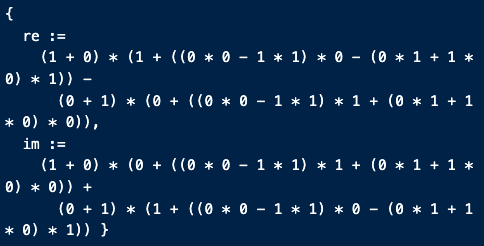
\includegraphics[width=0.95\linewidth]{Chapters/5_Lean/Images/norm_numI_parse_output.png}
    \caption{The Lean output of the steps shown in \Cref{Ch5:Eg:Parse}.}
    \label{Ch5:Fig:Parse_Example}
\end{wrapfigure}

Note that in Lean, the result of parsing does not appear as an expression of the form $a + bi$, but rather, as a \lstinline|structure| with fields \lstinline|re| and \lstinline|im| for the real and imaginary parts. However, the underlying idea is no different from what we have described.

Clearly, despite being mathematically valid, the result of parsing can be long and uninformative, making it an unsuitable choice of normal form for our purposes. However, by separating complex expressions into their real and imaginary parts, \lstinline|parse| perfectly sets up a very simple normalisation procedure that will put our expression in an appropriate normal form. Since we know of such a procedure for real expressions---namely, \lstinline|norm_num|---and since \lstinline|parse| expresses any complex expression as a combination of two real expressions, the normalisation procedure simply makes calls to \lstinline|norm_num| to express each of them in a \textit{real} normal form. The result is a complex number in a normal form $a + bi$ (or, in Lean notation, \lstinline|{re := a, im := b}|) with $a$ and $b$ both simplified to the greatest extent possible (as expressions in $\R$) by applying \lstinline|norm_num|.

Note that \lstinline|norm_numI| is currently implemented as a \lstinline|conv| tactic rather than a full tactic, meaning that it is only capable of modifying expressions (and providing a proof that the modification is valid). It is not currently capable of proving goals, which are necessarily logical statements, such as equalities. This means that it needs to be used as follows.

\begin{lstlisting}[caption=Using \lstinline|norm_numI| as a \lstinline|conv| tactic, label=Ch5:Listing:norm_numI_as_conv]
example : (1 + I) * (1 + I * I * I) = 2 := by
  conv_lhs => norm_numI
  conv_rhs => norm_numI
\end{lstlisting}

Unpacking the code,
\begin{itemize}
    \item \lstinline|conv_lhs => norm_numI| applies the parsing-normalisation procedure outlined above to convert the expression \lstinline|(1 + I) * (1 + I * I * I)| on the left-hand side to \lstinline|{re := 2, im := 0}|.
    \item \lstinline|conv_rhs => norm_numI| applies the parsing-normalisation procedure outlined above to convert the expression \lstinline|2| on the right-hand side to \lstinline|{re := 2, im := 0}|.
\end{itemize} 
Since the two sides are then exactly the same, the goal is proved. Note that both lines are necessary: $2$ on its own has not been separated into real and imaginary parts. The imaginary part needs to be explicitly shown to be $0$, which the \lstinline|parse| function does.

After Macbeth, Xie and the author's initial success with this \lstinline|conv| tactic, Macbeth proceded to create an \textit{extension} of the existing \lstinline|norm_num| tactic that uses the parsing technique outlined above to handle complex expressions. This tactic is still being developed, but is being tested on active code from the project with immensely promising results.

\subsection{Scope for Further Development}

The benefits of having such a tactic cannot be overstated. There are numerous instances across the project where the collaborators have had to repeatedly prove computational facts in $\C$, such as $1 + i \neq 0$, or clear complex denominators to separate expressions into their real and imaginary parts.

% Give an explicit example here from the repo

The applicability of \lstinline|norm_numI|---or, at the very least, of the underlying idea, that the right normal form for expressions in $\C$ is to separate them into real and imaginary parts and express those in a normal form---extends well beyond expressions in $\C$. A key motivation for Xie, one of the co-creators of \lstinline|norm_numI| and an ardent algebraist, was to create a similar tactic that would normalise and simplify expressions in quaternion algebras. A discussion at a London Learning Lean event hosted at the London Institute of Mathematical Sciences in March 2025 sparked speculation among well-regarded members of the Lean Community that similar ideas might be applicable in other field extensions (with $\C$ regarded as $\quotient{\R[X]}{\parenth{X^2 + 1}}$ and $i$ as the image of $X$ via the quotient map). The idea would be that the separation into components corresponds to taking advantage of some linear independence criterion, with algebraic dependences not handled by the simplification step being captured by the helper lemmas in the normalisation step.

There are numerous technical difficulties with implementing such a tactic that can work in other contexts, chief amongst them the fact that there would need to be a single modification to the tactic capable of handling very differently behaved algebraic structures (for instance, it would need to work the same way in quadratic, cubic, quartic and higher degree field extensions). It would hence need to have some awareness of the behaviours of each field in which it is applied, which is technically challenging. Nevertheless, the development of \lstinline|norm_numI| and the subsequent \lstinline|norm_num| modification marks a significant, and long overdue, step in the right direction, so that fewer nontrivial proofs are needed to prove trivial facts.
\section{The Cauchy-Goursat Theorem}
\label{Ch5:Sec:Cauchy-Goursat}

\begin{comment}
Maybe begin with an anecdote - no sooner had we entered Hales's office in Pittsburgh than he asked about how we plan to deform integration contours.

Have 3 subsections.
1. Informal maths
2. Discussion of existing formalisation of closed rectangular case, with emphasis on why we don't have it for other cases (cite Hales's formalisation of the Jordan Curve Theorem in HOL-Light, maybe try and explain why we don't have something similar in Lean)
3. Discussion of our approach to the indefinite case (informally and formally)
Also maybe find better words than closed/open? Because these words are NOT used here in a topological sense, but rather in a very visual sense ("are the two endpoints of the curve the same point or are they not? Does the curve even have two endpoints or does it just have one and then go off to i\infty in the other?")
\end{comment}

There are some areas of mathematics that are notoriously difficult to formalise. Algebra, for example, tends to be easier to formalise than analysis. Within analysis, it tends to be particularly difficult to formalise geometric ideas, and few are as deceptively challenging as the innocent-sounding \JCT. It was not until 2007 that this theorem, proposed in the late 19th Century, was formalised by Tom Hales \cite{JordanCurve} in HOL Light, and to this day, no formalisation exists in Lean. The author had the privilege of meeting Hales in Pittsburgh, USA, in March 2025 to discuss the formalisation of $8$-dimensional sphere packing in Lean, and the very first question Hales asked was what the strategy was to overcome the challenges of not having a Lean formalisation of the Jordan Curve Theorem.

The \JCT\ states that a simple closed curve $C \subset \R^2$, given as the image of a continuous injection from $\mathbb{S}^1$, divides $\R^2 \setminus C$ into a bounded region, known as the \textit{interior} of $C$, and an unbounded region, known as the \textit{exterior} of $C$. This gives us a clear way of stating the all-important holomorphicity condition of the \CGT: a path of integration can usually only be deformed if the integrand is holomorphic in the region enclosed by the two paths, and the \JCT\ defines this region. Viazovska uses versions of the \CGT\ to prove the eigenfunction property and the double zero property (see \Cref{Ch4:Sec:Eig,Ch4:Sec:Double_Zeroes}. Fortunately, in both instances, we have explicit contours. Hence, the regions where we require holomorphicity can both be defined, and it is easy to show the integrands are holomorphic in those regions.

This is a significant simplification because it means we have all the ingredients to \textit{state} the results we require. However, there are still challenges involved in proving them. We give a brief overview of the two cases of interest in the forthcoming subsections.

\subsection{Rectangles}

The following version of the \CGT\ had been \href{https://github.com/leanprover-community/mathlib4/blob/c38c7fde32656c7fa1b2471ed1ae0d50a600f089/Mathlib/Analysis/Complex/CauchyIntegral.lean#L241-L255}{formalised} prior to this project.

\begin{boxtheorem}[Cauchy-Goursat for Rectangles]\label{Ch5:Thm:CauchyGoursat_Bounded_on_off_Countable}
    Suppose $f : \C \to \C$ is a function such that $f(z) \to 0$ as $\Im(z) \to \infty$. Then, for all $x_1, y_1, x_2, y_2 \in \R$, if $f$ is holomorphic at all but countably many $z \in \C$ with $x_1 < \Re(z) < x_2$ and $y_1 < \Im(z) < y_2$ and continuous on the corresponding closed rectangle, then
    \begin{align*}
        \int_{x_1}^{x_2} f\of{x + y_1 i} \diff{x}
        - \int_{x_1}^{x_2} f\of{x + y_2 i} \diff{x}
        + i\int_{y_1}^{y_2} f\of{x_2 + yi} \diff{y}
        - i\int_{y_1}^{y_2} f\of{x_1 + yi} \diff{y} = 0
    \end{align*}
\end{boxtheorem}

The author was able to adapt this to the following unbounded version.

\begin{boxtheorem}[Cauchy-Goursat for Unbounded Contours]\label{Ch5:Thm:CauchyGoursat_Unbounded_on_off_Countable}
    Suppose $f : \C \to \C$ is a function such that $f(z) \to 0$ as $\Im(z) \to \infty$. Then, for all $x_1, x_2, y \in \R$, if $f$ is holomorphic at all but countably many $z \in \C$ with $x_1 < \Re(z) < x_2$ and $y < \Im(z)$ and then
    \begin{align*}
        \int_{y}^{\infty} f\of{x_1 + ti} \, \diff{t}
        = \int_{x_1}^{x_2} f\of{t + yi} \, \diff{t}
        + \int_{y}^{\infty} f\of{x_2 + ti} \, \diff{t}
    \end{align*}
    provided that the integrals along the vertical contours exist.
\end{boxtheorem}

\begin{wrapfigure}[12]{r}{0.4\linewidth}
    \vspace{-0.7em}
    \centering
    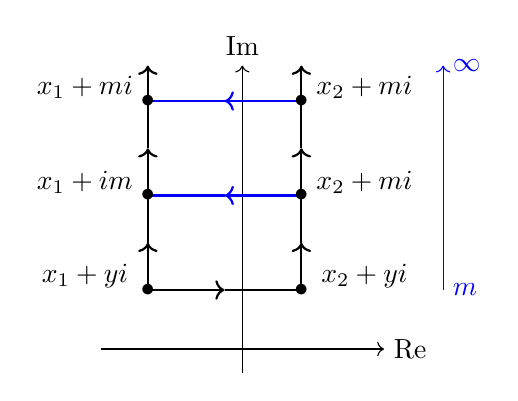
\begin{tikzpicture}[scale=1.5]
        % Axes
        \draw[->] (-1.2,0) -- (1.2,0) node[right] {$\Re$};
        \draw[->] (0,-0.2) -- (0,2.4) node[above] {$\Im$};
    
        % Contours
        % \draw[thick, ->] (-0.8,0.5) -- (-0.8, 2.4);
        % \draw[thick, ->] (0.5,0.5) -- (0.5, 2.4);
        %% Translation Contour
        \draw[thick, ->] (-0.8, 0.5) -- (-0.15, 0.5);
        \draw[thick] (-0.15, 0.5) -- (0.5, 0.5);
        %% Blue vanishing ones
        \draw[thick, blue] (-0.15, 1.3) -- (-0.8, 1.3);
        \draw[thick, ->, blue] (0.5, 1.3) -- (-0.15, 1.3);
        \draw[thick, blue] (-0.15, 2.1) -- (-0.8, 2.1);
        \draw[thick, ->, blue] (0.5, 2.1) -- (-0.15, 2.1);
        %% Vertical ones
        \draw[thick, ->] (-0.8, 0.5) -- (-0.8, 0.9);
        \draw[thick, ->] (0.5, 0.5) -- (0.5, 0.9);
        \draw[thick, ->] (-0.8, 0.9) -- (-0.8, 1.7);
        \draw[thick, ->] (0.5, 0.9) -- (0.5, 1.7);
        \draw[thick, ->] (-0.8, 1.7) -- (-0.8, 2.4);
        \draw[thick, ->] (0.5, 1.7) -- (0.5, 2.4);
    
        % Points of interest
        \labelledpoint{-0.8}{0.5}{-0.8}{-0.3}{$x_1 + yi$}
        \labelledpoint{0.5}{0.5}{0.8}{-0.3}{$x_2 + yi$}
        \labelledpoint{0.5}{1.3}{0.8}{-0.3}{$x_2 + mi$}
        \labelledpoint{0.5}{2.1}{0.8}{-0.3}{$x_2 + mi$}
        \labelledpoint{-0.8}{1.3}{-0.8}{-0.3}{$x_1 + im$}
        \labelledpoint{-0.8}{2.1}{-0.8}{-0.3}{$x_1 + mi$}

        % m \to \infty
        \draw[thin, ->, blue] (1.7, 0.5) node[right] {$m$} -- (1.7, 2.4) node[right] {$\infty$};
    \end{tikzpicture}
    \caption{The contours in \Cref{Ch5:Thm:CauchyGoursat_Unbounded_on_off_Countable}.}
    \label{Ch5:Fig:Unbounded_Contour}
\end{wrapfigure}

It is immediate that this implies \Cref{Ch4:Thm:CauchyGoursat_Unbounded}.

We briefly sketch a proof of \Cref{Ch5:Thm:CauchyGoursat_Unbounded_on_off_Countable}. Writing the integrals along both vertical contours as limits as $m \to \infty$ of the integrals from $y$ to $m$, we can apply \Cref{Ch5:Thm:CauchyGoursat_Bounded_on_off_Countable} to each rectangle with vertices $x_1 + yi$, $x_2 + yi$, $x_1 + mi$ and $x_2 + mi$ gives us two different expressions for the integral along $x_1$, one of which agrees with the integral along $x_2$ as $m \to \infty$ because the integrals along the blue contours in \Cref{Ch5:Fig:Unbounded_Contour} can be shown to vanish using the property that $f(z) \to 0$ as $\Im(z) \to \infty$.

The author has \sorry-free versions of this in the repository as well as one version with a \sorry. This is because the author is trying to minimise the number of assumptions required for \Cref{Ch5:Thm:CauchyGoursat_Unbounded_on_off_Countable}. For instance, integrability is stronger than the existence of the integrals, because integrability (in Lean) is a combination of absolute convergence and measurability. In the repository, these contours are currently referred to as open, not in a topological sense but in the sense that they do not consist of closed curves. Perhaps unbounded is a better term.

It was the fact that such a simple and elegant solution existed for deforming unbounded contours that motivated the definition of the $I_j$ and $J_j$ using rectangular contours. While circular contours would make the eigenfunction proof easier, the challenge of proving \Cref{Ch5:Thm:CauchyGoursat_Unbounded_on_off_Countable} would either involve reconciling circles and rectangles, which we discuss in the next subsection, or a direct proof, which the author expects would be immensely difficult to formalise.

We end this discussion by noting that the rectangles in \Cref{Ch5:Thm:CauchyGoursat_Bounded_on_off_Countable,Ch5:Thm:CauchyGoursat_Unbounded_on_off_Countable} have a particular orientation that makes it easier to define their interior. For rectangles oriented differently, it is conceivable that a proof involving variable changes can be formalised when an orientation is specified, but it will require effort.

\subsection{Squares and Circles}

To prove \Cref{Ch4:Sec:Eig}, we effectively need the following.

\begin{boxtheorem}[Cauchy-Goursat: Squares and Circles]\label{Ch5:Thm:CauchyGoursat_Circle_Rectangle}
    Fix $w \in \C$ and $r > 0$. Let $\gamma$ be the quarter-circle parametrised by $\gamma(t) = w + r\pcos{t} + r i \psin{t}$ for $0 \leq t \leq \pi/2$. Let
    \begin{align*}
        S = \setst{x + yi \in \C}{\parenth{x^2 + y^2 > r^2} \land \parenth{0 < x < r} \land \parenth{0 < y < r}}
    \end{align*}
    For any $f : \C \to \C$ that is holomorphic on all but countably many points in $S$ and continuous on the closure $\bar{S}$ of $S$,
    \begin{align*}
        \int_{\gamma} f(z) \, \diff{z}
        = \int_{w + r}^{w + r + ir} f(z) \, \diff{z} + \int_{w + r + ir}^{w + ir} f(z) \, \diff{z}
    \end{align*}
\end{boxtheorem}

\begin{wrapfigure}{r}{0.4\linewidth}
    \vspace{-0.7em}
    \centering
    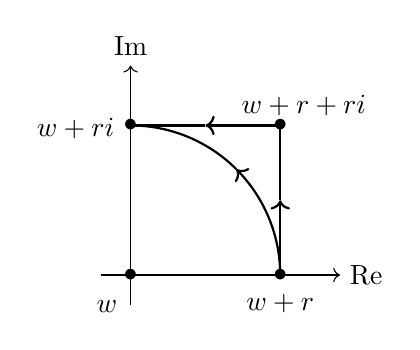
\begin{tikzpicture}[scale=1.9]
        % Axes
        \draw[->] (-0.2,0) -- (1.4,0) node[right] {$\Re$};
        \draw[->] (0,-0.2) -- (0,1.4) node[above] {$\Im$};
    
        % Quarter-circle contour
        \draw[thick, domain=0:45, ->] plot ({cos(\x)}, {sin(\x)});
        \draw[thick, domain=45:90, -] plot ({cos(\x)}, {sin(\x)});

        % Rectangular contour
        \draw[thick, ->] (1,0) -- (1,0.5);
        \draw[thick, -] (1,0.5) -- (1,1);
        \draw[thick, ->] (1,1) -- (0.5,1);
        \draw[thick, -] (0.5,1) -- (0,1);

        % % Dyadic style approximation
        % \foreach \n in {0, 1, 2, 3, 4, 5, 6, 7, 8, 9, 10} { % Depth
        %     \foreach \l in {1, ..., \n} { % Lines
                
        %     }
        % }

        % Points of interest
        \labelledpoint{0}{0}{-0.3}{-0.8}{$w$}
        \labelledpoint{1}{0}{0}{-0.8}{$w + r$}
        \labelledpoint{1}{1}{0.3}{-0.2}{$w + r + ri$}
        \labelledpoint{0}{1}{-0.7}{-0.5}{$w + ri$}
    \end{tikzpicture}
    \caption{The contours in \Cref{Ch5:Thm:CauchyGoursat_Circle_Rectangle}.}
    \label{Ch5:Fig:Square_Circle_Contour}
\end{wrapfigure}

Again, we are saved from the difficulties of applying the \JCT\ because we are working in a very specific situation where we can explicitly describe $S$. However, proving this result, formally and informally, is significantly more complicated than proving \Cref{Ch4:Thm:CauchyGoursat_Unbounded}. One proof would be to arbitrarily approximate $\gamma$ by squares of exponentially decaying side lengths. For any contour defined in this way, we can show, by inductively applying \Cref{Ch5:Thm:CauchyGoursat_Bounded_on_off_Countable}, that the integral along it equals the integral along the rectangular contour in \Cref{Ch5:Fig:Square_Circle_Contour}. Since these contours converge to $\gamma$ pointwise, it should be possible to show, by \href{https://github.com/leanprover-community/mathlib4/blob/c38c7fde32656c7fa1b2471ed1ae0d50a600f089/Mathlib/MeasureTheory/Integral/DominatedConvergence.lean#L49-L63}{dominated convergence}, that the (constant) sequence of integrals along the square contours converges to the integrals along $\gamma$.

Unfortunately, these ideas are incredibly difficult to formalise, not least because it is difficult to define such a sequence of parametrisations in Lean. Other possible approaches include formalising a version for triangles and subsequently approximating the circle using triangles. Regardless of the approach, formalising \Cref{Ch5:Thm:CauchyGoursat_Circle_Rectangle} will be a challenge. If done successfully, however, it will be a significant achievement in itself as well as a valuable contribution to this project.
\chapter{Conclusion}
\label{Ch6:Chapter}
\thispagestyle{empty}

Over the course of this thesis, we have explored a revolutionary approach to a classical problem that has since led to deep insights into the mysteries of the $E_8$ lattice, its $24$-dimensional counterpart, the Leech lattice, and the broader theory of radial Schwartz functions. Previously unexplored links to the theory of modular forms have since revealed deep symmetries that have led to fascinating results, such as Cohn, Kumar, Miller, Radchenko and Viazovska's universal optimality and Fourier interpolation formulas \cite{UniversalOptimality} that reconstruct radial Schwartz functions $f$ from the values and radial derivatives of $f$ and $\hat{f}$, generalising Viazovska's approach to solving the sphere packing problem in $\R^8$.

The advent of formalisation marks the beginning of an epistemological revolution that will solidify the certainty with which use and build on existing results. The formalisation of Viazovska's groundbreaking work could not come at a better time: we stand at the precipice of innumerable possibilities, informal and formal, and a complete, \sorry-free verification of Viazovksa's work would be a vote of confidence that both fields are progressing in the right direction.

In the sections below, we summarise the author's key takeaways at the end of this project.

\section{Viazovska's Monumental Breakthrough}

It is with good reason that Cohn writes,
\begin{quote}
    Overall, this proof feels like a miracle.Everything falls beautifully into place, with Viazovska’s constructions having just enough flexibility to complete the proof in a unique way. \ldots Viazovska is a master of special functions, whose work would surely have excited Jacobi and Ramanujan
\end{quote}
\cite[p.21]{CohnOnViazovskaICM}. Viazovska's ingenuity stems from the manner in which she overcame the difficulties in controlling funtions and their Fourier transforms simultaneously: realising that the magic function would need to be an integral transform and that the function being transformed would need to admit numerous change of variable properties, she tapped into the theory of modular forms to find precisely such a function.

Over the course of this thesis, we have explored the specifics of the solution. The first important insight were the linear programming bounds on sphere packing densities, which reduced a famously difficult geometric problem into a deceptively difficult analytic problem. The second was that there exist a remarkable class of functions, encountered in \Cref{Ch2:Sec:ModForms}, that obey numerous transformation rules that make them perfect candidates for navigating the symmetries of Möbius changes of variables. We began to get an inkling of their relevance when we observed, in \Cref{Ch3:Chapter}, that the problem of finding a magic function for the Cohn-Elkies bounds could be divided into two problems: finding $\pm 1$-Fourier eigenfunctions with double zeroes at lattice points and expressing them as an appropriate linear combination. We further established the relevance of the theory of modular forms by conceiving that their numerous change of variable properties might make them good candidates for integral transforms to construct the eigenfunctions. In \Cref{Ch4:Chapter}, we saw that Viazovska did something similar: she combined functions that were either modular forms or closely enough related to obey similar properties to form Schwartz functions that were well-behaved under precisely those variable changes needed to relate them to their Fourier transforms. We discussed her construction in tremendous detail, identifying previously formalised results that can be used in our formalisation as well as gaps in \mathlib\ that would need to be filled to successfully formalise Viazovska's result. Finally, in \Cref{Ch5:Chapter}, we gave an overview of techniques developed thus far in the formalisation to overcome some, though admittedly not all, of the difficulties identified in \Cref{Ch4:Chapter}.

Each step in Viazovska's construction was meticulously thought out, resting on two robust, well-developed areas of study: modular forms and radial Schwartz functions. The Schwartzness proof is particularly interesting: the applicability of \Cref{SP:PolyFourierCoeffBound} to modular forms and similar functions to construct bounds on their absolute values and those of their integral transforms is a powerful bridge between the two seemingly unrelated areas. One wonders what new mysteries will be unearthed as Viazovska and her collaborators continue to explore this rich region in the even richer tapestry of modern mathematics.
\section{The Road to Formalising Sphere Packing}
% \section{A Glance Ahead}

The fact that \mathlib\ is at a stage where it is even possible to envision a formalisation of such recent and revolutionary work as Viazovska's already says volumes about the progress in formalisation over the last decade. Moreover, it is a testament to the power of open-source collaboration: every day, strides are being made by countless contributors worldwide that enhance the capabilities of Lean and the vastness of \mathlib, making for a more efficient and enjoyable formalisation experience. It is to harness the power of this community and to mobilise enthusiasts and experts to contribute to this project that the collaborators, represented by Viazovska herself, have decided to make the repository public on 13 June, 2025, at Cambridge.

Beyond the specifics of this project, the goals as well as the accomplishments thus far have a wide range of applications. For example, the author's bridge between dimensions involving Schwartz-like functions, seen in \Cref{Ch5:Subsec:Schwartz_Bridge}, and the fact that the Schwartz-like behaves nicely with linear combinations, as used in \Cref{Ch4:Sec:Schwartzness} to prove that $a\rad$ and $b\rad$ are Schwartz-like, suggests that there may be a deeper theory waiting to be explored, an exciting prospect so soon after Viazovska added a revolutionary new perspective to the theory of Schwartz functions. On the formal front, the development of \lstinline|norm_numI| at a time when there is much discussion on improving automation in a variety of algebraic settings could lead to further improvements being made to existing tactics, potentially leading to the development of polymorphic automation, where normalisations and simplifications understand and depend on the setting. Furthermore, just as this project catalysed the development of \lstinline|norm_numI|, so too may it catalyse formalisations of results like the \CGT\ and potentially even the \JCT, so that future formalisers can sidesteps the vexation faced by the author when dealing with contour integrals. Finally, the systematic approach taken by the author to bound integrals formally demonstrates that a certain degree of systematisation is possible, and the author's growing understanding of metaprogramming has led to the birth---though not much more---of ideas that would make formal integral calculations more user-friendly.

The road ahead may be uncertain, but it is safe to say it is filled with potential. In conclusion, the end of this M4R is only the beginning.

The end of this M4R is only the beginning.

% \appendix
% \chapter{First Appendix}

%%%%%%%%%%%%%%%%%%%%%%%%%%%%%%%%%%%%%
\bibliography{References/bibliography.bib}
% \thispagestyle{empty}
%%%%%%%%%%%%%%%%%%%%%%%%%%%%%%%%%%%%%

\end{document}